\article{局部域上的约化群}{Reductive Groups over Local Fields}{J. Tits}{1}{29--69}
\paragraph*{篇内目录（原书页码）}
0. 预备知识，30；0.1 引言，30；0.2 记号，30。

1. 极大分裂环面的公寓与仿射根系，31；1.1 分裂情形，31；1.2 公寓 $A(G,S,K)$，31；1.3 注记，32；1.4 群 $U_a(K)$ 的滤过，32；1.5 关于证明、参考文献及推广，33；1.6 仿射根系 $\Phi_{\mathrm{af}}$，33；1.7 半公寓、室、仿射 Weyl 群，33；1.8 基、局部 Dynkin 图、特征维数，34；1.9 与 $A$ 的点相联系的根系和特殊点，35；1.10 域扩张下的行为与超特殊点，36；1.11 绝对与相对局部 Dynkin 图；指标，37；1.12 约化到绝对拟单情形；标量限制，38；1.13 单连通群的情形，39；1.14 例：一般线性群，39；1.15 例：奇数维拟分裂特殊酉群，40；1.16 例：拟分裂但不分裂的正交群，42。

2. 建筑，43；2.1 定义，43；2.2 $\mathscr I$ 上的仿射结构、面、收缩、拓扑与其他典范结构，44；2.3 度量与单纯形分解，45；2.4 Dynkin 图；特殊点与超特殊点，45；2.5 $(\Aut G)(K)$ 在 $\mathscr I$ 与 $\Delta$ 上的作用；特殊点与超特殊点的共轭类，46；2.6 域扩张下的行为，47；2.7 例：相对秩为一的群，48；2.8 例：$\SL_3$ 与 $\GL_3$，48；2.9 例：一般线性群，49；2.10 例：特殊酉群，49。

3. 稳定子与中心化子，50；3.1 记号：一个 BN 对，50；3.2 极大有界子群，50；3.3 各种分解，51；3.4 若干群概形，51；3.5 模 $\mathfrak p$ 约化，52；3.6 环面单位群的不动点，54；3.7 Iwahori 子群；极大紧子群的体积，54；3.8 超特殊点与子群，55；3.9 整体情形，55；3.10 例：一般线性群，56；3.11 例：奇数维拟分裂特殊酉群，56；3.12 例：拟分裂但不分裂的特殊正交群，58。

4. 分类，59；4.1 引言，59；4.2 剩余分裂群，60；4.3 非剩余分裂群，62；4.4 解释，67；4.5 不变量，68；4.6 分类工具包，68。参考文献，68。
\footnotetext{AMS（MOS）学科分类（1970）：主要分类 20G25；次要分类 20G30、15A63。}

\origsection{0}{预备知识（Preliminaries）}
\origsubsection{0.1}{引言（Introduction）}
本文综述局部域（local fields）上约化群（reductive groups）结构理论的若干方面。文章主要面向需要应用这些结果的读者，因此着重陈述结论、介绍例子。为帮助读者理解理论中的关键环节，文中会保留一些简短论证，其余证明大多省略。已有证明的结果会注明出处；部分结果的证明当时尚未发表；对 [8] 的引用常有条件限制，见 1.5。

这里仅简要交代理论的发展背景：此理论由 N. Iwahori 和 H. Matsumoto [15] 开创，他们研究的是分裂半单群（split semisimple groups）；H. Hijikata [13] 随后研究拟分裂群（quasi-split groups）与经典群；在本文的一般范围内，多数结果归功于 F. Bruhat 与作者 [6]、[7]、[8]、[9]。更多背景可参看 [8] 的引言。
\origsubsection{0.2}{记号（Notations）}
全文采用以下记号：$K$ 为带非平凡离散赋值（discrete valuation）$\omega$ 的域，值群 $\omega(K^\times)\subset\R$ 也记作 $\Gamma$；$\mathfrak o$ 表示整数环，$\mathfrak p=\pi\mathfrak o$（$\pi\in\mathfrak o$）为其极大理想，$\overline K=\mathfrak o/\mathfrak p$ 为剩余域。始终假定 $K$ 完备且 $\overline K$ 完美（perfect）。考虑在 $K$ 上定义的代数群 $G$，其单位连通分支（neutral component）$G^\circ$ 约化。以 $S$ 表示 $G$ 的极大 $K$ 分裂环面（maximal $K$-split torus）；$N$、$Z$ 分别为 $S$ 在 $G$ 中的正规化子（normalizer）与中心化子（centralizer）；$\prescript{v}{}{\widetilde W}=N(K)/Z(K)$ 为有限群。（通常，$?(K)$ 表示对象 $? $ 的 $K$ 有理点群。）
\[
X^*=X^*(S)=\Hom_K(S,\operatorname{Mult}),\qquad
X_*=X_*(S)=\Hom_K(\operatorname{Mult},S)
\]
分别为 $S$ 的特征群（characters）与余特征群（cocharacters）；$V=X_*\otimes\R$ 为实向量空间；$\Phi=\Phi(G,S)\subset X^*$ 为 $G$ 相对于 $S$ 的根集合；$\prescript{v}{}{W}$ 为根系（root system）$\Phi$ 的 Weyl 群，它可自然视为 $\prescript{v}{}{\widetilde W}$ 的一个正规子群（若 $G=G^\circ$，则二者相等）；对 $a\in\Phi$，$U_a$ 为 $G^\circ$ 的由 $S$ 正规化并对应于根 $a$ 的幺幂子群（unipotent subgroup），即 [3，5.2] 中记为 $U_{(a)}$ 的群。

\origsection{1}{极大分裂环面的公寓与仿射根系（The apartment of a maximal split torus and the affine root system）}
\origsubsection{1.1}{分裂情形（The split case）}
为说明下面讨论的动机，先考虑 $G^\circ$ 分裂的情形，即 $S$ 为 $G$ 的极大环面。这时，群 $U_a$ 在 $K$ 上同构于加法群。事实上，在 $G$ 的 Lie 代数中选取一个“Chevalley 基”，就确定一组 $K$ 同构 $\chi_a:\operatorname{Add}\to U_a$（一个钉扎，pinning，原文为 épinglage），满足 Chevalley 的交换关系 [10，第 27 页]。$K$ 的赋值为其加法群给出了自然滤过；通过上述同构，这一滤过也成为 $U_a(K)$ 上的滤过。用 $V$ 上的仿射函数（affine functions）标记滤过的各项十分方便：若 $a\in\Phi$、$\gamma\in\Gamma$，则 $a+\gamma$ 为这样的函数，令
\[
X_{a+\gamma}=\chi_a(\omega^{-1}[\gamma,\infty]).\tag{1.1(1)}
\]
若对某个 $s\in S(K)$ 用 $\Ad s$ 变换 Chevalley 基，则同构族 $(\chi_a)$ 变为 $(\chi'_a)=(\chi_a\circ a(s))$。令 $X'_{a+\gamma}=\chi'_a(\omega^{-1}[\gamma,\infty])$，则
\[
X'_{a+\gamma}=X_{a+\gamma+\omega(a(s))}.\tag{1.1(2)}
\]
所以，群 $U_a(K)$ 的滤过各项保持不变，但其编号发生了平移。对 Chevalley 基的任意改变，也有相同结论（只需将 $s$ 替换为 $S$ 在伴随群中的像的一个有理元素）。

这一结论可以用不依赖坐标的方式表述：存在以 $V$ 为平移空间的仿射空间（affine space）$A$、$A$ 上的仿射函数系统 $\Phi_{\mathrm{af}}$，以及从 $\Phi_{\mathrm{af}}$ 到 $G(K)$ 的某组子群上的映射 $\alpha\mapsto X_\alpha$，满足：每个 Chevalley 基对应于点 $0\in A$，使 $\Phi_{\mathrm{af}}$ 由所有函数
\[
\alpha:x\longmapsto a(x-0)+\gamma,\qquad x\in A,\ a\in\Phi,\ \gamma\in\Gamma,\tag{1.1(3)}
\]
构成；若 $(\chi_a)$ 为与给定基对应的钉扎，则与函数（3）对应的群 $X_\alpha$ 由（1）给出。群 $S(K)$ 通过平移作用于 $A$，使对 $s\in S(K)$ 有
\[
s^{-1}X_\alpha s=X_{\alpha\circ s}.\tag{1.1(4)}
\]
由（2），$s$ 在 $A$ 上诱导的平移 $\nu(s)\in V$（由 $s(x)=x+\nu(s)$，$x\in A$，定义）满足
\[
a(\nu(s))=-\omega(a(s)),\qquad\text{对每个 }a\in\Phi.\tag{1.1(5)}
\]
更一般地，$S(K)$ 在 $G(K)$ 中的正规化子 $N(K)$ 通过仿射变换作用于 $A$，使（4）对任意 $s\in N(K)$ 成立。
\origsubsection{1.2}{公寓 A(G,S,K)（The apartment A(G,S,K)）}
下面要将上述构造推广到一般的 $G$：为 $G,S,K$ 构造一个以 $V$ 为平移空间、带有 $N(K)$ 作用的仿射空间 $A=A(G,S,K)$，一个 $A$ 上的仿射函数系统 $\Phi_{\mathrm{af}}=\Phi_{\mathrm{af}}(G,S,K)$，以及从 $\Phi_{\mathrm{af}}$ 到 $G(K)$ 的某组子群上的映射 $\alpha\mapsto X_\alpha$，使关系 1.1（4）对 $s\in N(K)$ 成立，使函数 $\alpha\in\Phi_{\mathrm{af}}$ 的向量部分（vector parts）$v(\alpha)$ 正好是 $\Phi$ 的元素，并使对 $a\in\Phi$，满足 $v(\alpha)=a$ 的群 $X_\alpha$ 构成 $U_a(K)$ 的滤过。

先构造空间 $A$；集合 $\Phi_{\mathrm{af}}$ 与各 $X_\alpha$ 将在 1.6 和 1.4 定义。关系（5）提示了这一构造的方向。$Z$ 的 $K$ 有理特征群 $X^*(Z)$ 可等同于 $X^*$ 的有限指数子群。定义同态 $\nu:Z(K)\to V$，使
\[
\chi(\nu(z))=-\omega(\chi(z)),\qquad z\in Z(K),\ \chi\in X^*(Z),\tag{1.2(1)}
\]
并以 $Z_c$ 表示 $\nu$ 的核。于是 $\Lambda=Z(K)/Z_c$ 是秩为 $\dim S=\dim V$ 的自由交换群。商 $\widetilde W=N(K)/Z_c$ 是有限群 $\prescript{v}{}{\widetilde W}$ 被 $\Lambda$ 的扩张。因此，存在以 $V$ 为平移空间的仿射空间 $A=A(G,S,K)$，以及 $\nu$ 到 $N(K)$ 的延拓，其值域为 $A$ 的仿射变换群，仍记作 $\nu$。若 $G$ 半单，则二元组 $(A,\nu)$ 是典范的，即在唯一同构意义下唯一。否则，它仅在同构意义下唯一；但可以依照 G. Rousseau [19]，以下述方式使其典范化：以 $\mathscr DG^\circ$ 表示 $G^\circ$ 的导出群（derived group），以 $S_1$ 表示 $G^\circ$ 的中心的极大分裂环面，取
\[
A=A(\mathscr DG^\circ,G^\circ\cap S,K)\times(X_*(S_1)\otimes\R),
\]
其中第一项是典范的。\footnote{\textbf{译者注（本次校订）：}第一项中第二个参数应为 $\mathscr DG^\circ\cap S$，即导出群的极大分裂环面；$G^\circ\cap S=S$ 一般并不包含在 $\mathscr DG^\circ$ 中。例如 $G=\GL_n$ 时，$S$ 的维数为 $n$，而 $\SL_n$ 的极大分裂环面维数为 $n-1$。}仿射空间 $A$ 称为 $S$（相对于 $G,K$）的公寓（apartment）。群 $N(K)$ 通过 $\widetilde W$ 作用于 $A$。
\origsubsection{1.3}{注记（Remark）}
由于 $V=\Hom(X^*,\R)=\Hom(X^*(Z),\R)$，群 $\Hom(X^*,\Gamma)$ 与 $\Hom(X^*(Z),\Gamma)$ 是 $V$ 中的格（lattices），且
\[
\Hom(X^*,\Gamma)\subset\nu(Z(K))=\Lambda\subset\Hom(X^*(Z),\Gamma).\tag{1.3(1)}
\]
如果 $G$ 连通且分裂，两个包含关系均为等号；一般情况下，它们可以是真包含。例如，设 $G=R_{L/K}\operatorname{Mult}$，其中 $L/K$ 为 $n$ 次可分扩张，令 $\Gamma_1$ 为 $L$ 的值群。群 $X^*(Z)$ 由范数同态 $N_{L/K}$ 生成，因此在 $X^*$ 中指数为 $n$。另一方面，容易看出 $\Lambda=n\Hom(X^*(Z),\Gamma_1)$。特别地，（1）的第一个（第二个）包含为等号，当且仅当扩张 $L/K$ 非分歧（完全分歧）。分裂域为 $L$ 的 $G=\operatorname{SU}_3$ 给出一个半单的例子：上述 $n=2$ 时的结论同样适用（事实上，此时 $Z=R_{L/K}\operatorname{Mult}$）。可以证明，只要 $G$ 在 $K$ 的某个非分歧扩张上分裂，第一个包含关系（1）就为等号。
\origsubsection{1.4}{群 Ua(K) 的滤过（Filtration of the groups Ua(K)）}
设 $a\in\Phi$、$u\in U_a(K)\setminus\{1\}$。已知（参见 [3，第 5 节]），交集 $U_{-a}uU_{-a}\cap N$ 只含一个元素 $m(u)$，它在 $\prescript{v}{}{\widetilde W}$ 中的像为对应于 $a$ 的反射（reflection）$r_a$。因此 $r(u)=\nu(m(u))$ 是向量部分为 $r_a$ 的仿射反射（affine reflection）。以 $\alpha(a,u)$ 表示 $A$ 上向量部分为 $a$、零超平面为 $r(u)$ 的不动点集的仿射函数；以 $\Phi'$ 表示向量部分属于 $\Phi$ 的全部仿射函数集合。对 $\alpha\in\Phi'$，令
\[
X_\alpha=\{u\in U_a(K)\mid u=1\text{ 或 }\alpha(a,u)\geq\alpha\}.
\]
下面两个结果是后续理论的基础。

\paragraph*{1.4.1.}对上述每个 $\alpha$，$X_\alpha$ 为群。

\paragraph*{1.4.2.}若 $\alpha,\beta\in\Phi'$，则交换子群（commutator group）$(X_\alpha,X_\beta)$ 包含于由所有 $X_{p\alpha+q\beta}$ 生成的群中，其中 $p,q\in\mathbb N^*$、$p\alpha+q\beta\in\Phi'$。\footnote{\textbf{译者注（本次校订）：}这一交换子公式须要求 $v(\alpha)$ 与 $v(\beta)$ 不互为负倍数。反向根子群的交换子还会产生环面部分。例如在 $\SL_2$ 中，取 $\alpha=a+\omega(\pi)$、$\beta=-a+\omega(\pi)$，两根子群中参数为 $\pi$ 的元素的交换子，其对角元在模 $\pi^3$ 后仍有 $\pi^2$ 项；而右侧所列根子群的参数都属于 $\pi^3\mathfrak o$。}

显然，满足 $v(\alpha)=a$ 的 $X_\alpha$ 构成 $U_a(K)$ 的滤过。以 $X_{\alpha+}$ 表示所有 $X_{\alpha+\varepsilon}$，$\varepsilon\in\R$、$\varepsilon>0$，之并（当然，当 $\varepsilon$ 足够小时，$X_{\alpha+}=X_{\alpha+\varepsilon}$）。由 1.4.2，$X_{\alpha+}$ 是 $X_\alpha$ 的正规子群，令 $\overline X_\alpha=X_\alpha/X_{\alpha+}$。因此，满足 $v(\alpha)=a$ 的 $\overline X_\alpha$ 是上述 $U_a(K)$ 滤过的各次分次商。显然，对 $n\in N(K)$ 有 $n^{-1}X_\alpha n=X_{\alpha\circ\nu(n)}$。
\origsubsection{1.5}{关于证明、参考文献及推广（About proofs, references and generalizations）}
选定一个“原点”$0$，将 $A$ 与 $V$ 等同，并对每个 $a\in\Phi$、$u\in U_a(K)$，令 $\varphi_a(u)=\alpha(a,u)-a\in\R$。断言 1.4.1 与 1.4.2 的实质是：函数族 $(\varphi_a)_{a\in\Phi}$ 是根数据（root datum）$(Z(K);(U_a(K))_{a\in\Phi})$ 的赋值，定义见 [8，6.2]。这一事实本身大致等价于（实际上稍强于）在全部 $U_a(K)$ 生成的群中存在某个 BN 对（BN-pair）（参见 [8，6.5 和 6.2.3(e)]），以及 $G$ 在 $K$ 上的仿射建筑（affine building）的存在（参见下文第 2 节和 [8，第 7 节]）。这些结果已在 [6]、[7]、[8，6.2.3(c)] 中宣布，但 Bruhat 与作者尚未发表完整证明（尽管经典群情形在 [8，第 10 节] 中已完全处理，拟分裂群也基本由 [8，9.2.3] 处理）。在此期间，H. Hijikata [14] 与 G. Rousseau [19] 发表了密切相关结果的证明。

后文许多结果都引用 [8]。这些引用通常表示：以 1.4.1 和 1.4.2 为前提，便可从所引章节得到相应结果的证明。

为简便起见，我们假定 $\omega$ 离散且 $\overline K$ 完美。事实上，只要 1.4.1 和 1.4.2 成立，到 3.3 为止的大部分陈述，经过适当改写，在去掉这些假设后仍然成立。已证明这两个断言总是成立；可能的例外只有 $\operatorname{char}\overline K=2$，且某些群 $G$ 的半单部分含有例外型、相对秩不超过 $2$ 的因子的情形（参见 [8，第 10 节]、[25] 与 [19]）。
\origsubsection{1.6}{仿射根系 Φaf（The affine root system）}
对 $A$ 上向量部分 $a=v(\alpha)$ 属于 $\Phi$ 的每个仿射函数 $\alpha$，显然有包含 $\overline X_{2\alpha}\hookrightarrow\overline X_\alpha$（若 $2a\notin\Phi$，令 $\overline X_{2\alpha}=\{1\}$）。商 $\overline X_\alpha/\overline X_{2\alpha}$ 自然具有 $\overline K$ 向量空间结构（参见 3.5.1），其维数有限，记为 $d(\alpha)$。特别地，若 $\operatorname{char}\overline K=p$，则 $\overline X_\alpha$ 为 $p$ 群。

若仿射函数 $\alpha$ 的向量部分 $a=v(\alpha)\in\Phi$，且 $d(\alpha)\ne0$，则称其为 $G$（相对于 $S,K$）的一个仿射根（affine root）；换言之，对任意严格正的常数 $\varepsilon$，$X_\alpha$ 不包含于 $X_{\alpha+\varepsilon}\cdot U_{2a}(K)$（当 $2a\notin\Phi$ 时，后者为 $X_{\alpha+\varepsilon}$）。以 $\Phi_{\mathrm{af}}(G,S,K)=\Phi_{\mathrm{af}}$ 表示 $G$ 的仿射根系，即全部仿射根的集合。注意，若 $2a\notin\Phi$，则对每个 $u\in U_a(K)\setminus\{1\}$，有 $\alpha(a,u)\in\Phi_{\mathrm{af}}$；特别地，若 $\Phi$ 约化（reduced），则
\[
\Phi_{\mathrm{af}}=\{\alpha(a,u)\mid a\in\Phi,\ u\in U_a(K)\setminus\{1\}\}.
\]
\origsubsection{1.7}{半公寓、室、仿射 Weyl 群（Half-apartments, chambers, affine Weyl group）}
对每个向量部分 $a=v(\alpha)\in\Phi$ 的仿射函数 $\alpha$，以 $A_\alpha$ 表示集合 $\alpha^{-1}([0,\infty))$，以 $\partial A_\alpha$ 表示其边界 $\alpha^{-1}(0)$，以 $r_\alpha$ 表示向量部分为反射 $r_a$（见 1.4）、不动超平面为 $\partial A_\alpha$ 的仿射反射。$\alpha\in\Phi_{\mathrm{af}}$ 对应的集合 $A_\alpha$（相应地，$\partial A_\alpha$）称为 $A$ 的半公寓（half-apartments）（墙，walls）；室（chambers）定义为 $A$ 中全部墙之并的补集的连通分支。室的面（facets）也称为 $A$ 的面；因此室为维数最大的面。若 $G$ 拟单（quasi-simple），各面（特别是室）为单纯形（simplices）；若 $G$ 半单，各面为多单纯形（polysimplices），即单纯形的直积；一般情形，各面是一个多单纯形与一个实仿射空间的直积。

由所有 $\alpha\in\Phi_{\mathrm{af}}$ 的 $r_\alpha$ 生成的群 $W$ 称为仿射根系 $\Phi_{\mathrm{af}}$ 的 Weyl 群。（如果 $G$ 不半单，这一用语略有滥用，因为 $W$ 不仅依赖于 $\Phi_{\mathrm{af}}$，也依赖于由 $X_*(\mathscr DG^\circ\cap S)$ 生成的 $V$ 的子空间，其中 $\mathscr DG^\circ$ 为 $G^\circ$ 的导群。）若 $G$ 半单，则 $W$ 是某个约化根系的仿射 Weyl 群（参见 [5，VI.2.1]），其元素分别与 $\Phi$ 的元素成比例，但该根系本身未必与 $\Phi$ 成比例，即使 $\Phi$ 约化也是如此（参见 1.15、1.16 的例子）。

显然，$\Phi_{\mathrm{af}}$ 在群 $\widetilde W=\nu(N(K))$ 下稳定（见 1.2）。因此，$\widetilde W$ 置换半公寓、墙和室，而且 $W$ 是 $\widetilde W$ 的正规子群。
\origsubsection{1.8}{基、局部 Dynkin 图、特征维数（Bases, local Dynkin diagram, characteristic dimensions）}
Weyl 群 $W$ 在所有室的集合上单可迁地作用（simply transitive），即传递地置换各室，且室在 $W$ 中的稳定子只有单位元。设 $C$ 为一个室，$L_0,\ldots,L_l$ 为界定 $C$ 的各墙。对 $i\in\{0,\ldots,l\}$，令 $\alpha_i$ 为满足 $L_i=\partial A_{\alpha_i}$、$\frac12\alpha_i\notin\Phi_{\mathrm{af}}$ 的唯一仿射根。\footnote{\textbf{译者注（本次校订）：}还须加上 $\alpha_i$ 在室 $C$ 内为正的条件，才能确定符号。否则 $\alpha_i$ 与 $-\alpha_i$ 有同一零超平面，并同时满足所写的不可除条件。}集合 $\{\alpha_i\mid i=0,\ldots,l\}$ 称为与 $C$ 对应的 $\Phi_{\mathrm{af}}$ 的基（basis）。

令 $a_i$ 为 $\alpha_i$ 的向量部分，在 $V$ 的对偶空间引入一个在（通常的）Weyl 群 $\prescript{v}{}{W}$ 下不变的正定内积 $(\ ,\ )$。按下述方式为 $\Phi_{\mathrm{af}}$ 定义一个（局部）Dynkin 图（local Dynkin diagram）$\Delta=\Delta(\Phi_{\mathrm{af}})$：

基的元素 $\alpha_i$ 以点 $v_i$ 表示，称为图的顶点（vertices）；若 $2\alpha_i\in\Phi_{\mathrm{af}}$，在顶点 $v_i$ 上标叉；

两个不同顶点 $v_i,v_j$ 之间，依整数
\[
\lambda_{ij}=\frac{4(a_i,a_j)^2}{(a_i,a_i)(a_j,a_j)}
\]
为 $0,1,2,3,4$，分别不连边、连单线、双线、三线或粗线（图的边，edges）；最后一种情形，$a_j$ 为 $-a_i$ 的正倍数；

如果 $\lambda_{ij}=2$ 或 $3$（这蕴涵 $(a_i,a_i)\ne(a_j,a_j)$），或者 $\lambda_{ij}=4$ 且 $a_j\ne-a_i$，则将连接 $v_i,v_j$ 的边加箭头，指向两个根 $a_i,a_j$ 中较“短”的那个根对应的顶点。

由于 $W$ 在室集上的作用单可迁，得到：

\paragraph*{1.8.1.}在典范同构意义下，Dynkin 图与室 $C$ 的选择无关。

容易看出，二元组 $(A,\Phi_{\mathrm{af}})$ 在同构意义下由 Dynkin 图 $\Delta$ 与 $A$ 的维数（即 $G$ 的相对秩）确定。Dynkin 图所对应的 Coxeter 图（Coxeter diagram），即忽略叉号与箭头所得的图，是 $W$ 的 Coxeter 图，因此是一个仿射反射群的 Coxeter 图（参见 [5，V.3.4 和 VI.4.3]，其中本文的“图”称为 graphes）。

反过来，考虑任意仿射反射群的 Coxeter 图，将所有双线和三线、以及可能的某些粗线定向，并在某些顶点上标叉（也可一个都不标）。则所得图是某个域 $K$ 上某个群 $G$ 的局部 Dynkin 图 $\Delta$，当且仅当每个标叉顶点 $v$ 所接的所有边均为双线或粗线，且没有一条定向边背离 $v$。

此条件的必要性显然。至于充分性，第 4 节的分类甚至表明：对给定的任意局部紧局部域 $K$，满足上述条件的每个图，都是某个 $K$ 上半单群 $G$ 的局部 Dynkin 图。事实上，列出所有这样的不可约图并不难，随即可见它们都出现在第 4 节的表中。注意，上述陈述，或第 4 节的表，给出了全部仿射根系的分类；只需给出仿射根系的适当抽象定义，有兴趣的读者可据此整理出相应的公理（也参见 [8，1.4]，其中仿射根系称为 échelonnages；约化情形见 [17]）。

若 $\Delta$ 的顶点 $v$ 代表仿射根 $\alpha$，令 $d(v)=d(\alpha)+d(2\alpha)$（若 $2\alpha\notin\Phi_{\mathrm{af}}$，则为 $d(\alpha)$），其中函数 $d$ 如 1.6 定义。整数 $d(v)$ 当然不仅依赖于 $\Delta,v$，还依赖于群 $G$ 本身。第 4 节各表中，凡 $d(v)\ne1$，都标明其数值。如果 $G$ 分裂或剩余域 $\overline K$ 代数闭，则所有 $d(v)$ 都等于 $1$。
\origsubsection{1.9}{与 A 的点相联系的根系和特殊点（Root system attached to a point of A and special points）}
对 $x\in A$，以 $\Phi_x$ 表示由在 $x$ 处消失的所有仿射根的向量部分构成的 $\Phi$ 的子集，以 $W_x$ 表示所有满足 $\alpha\in\Phi_{\mathrm{af}}$、$\alpha(x)=0$ 的反射 $r_\alpha$ 生成的群（见 1.7）。再按下述方式为 $x$ 指定局部 Dynkin 图 $\Delta$ 的一个顶点集 $I_x$：存在 Weyl 群 $W$ 的元素 $w$，将 $x$ 带入“基本室”（fundamental chamber）$C$ 的闭包，沿用 1.8 的记号，令 $I_x=\{v_i\mid wx\notin L_i\}$。$I_x$ 与 $w$ 的选择无关，这由 Coxeter 群的熟知性质得到，例如参见 [5，V.3.3，命题 1]。对象 $\Phi_x,W_x,I_x$ 只依赖于包含 $x$ 的面 $F$，也分别记为 $\Phi_F,W_F,I_F$。

集合 $\Phi_x$ 是 $\Phi$ 的一个（未必闭的）子根系，其 Weyl 群为 $W_x$ 的向量部分，其（通常的）Dynkin 图由 $\Delta$ 删去 $I_x$ 中的顶点及与之相接的边得到。集合 $I_x$ 与 $\Delta$ 的每个连通分支都有交点；反之，具有此性质的每个顶点集，都是某个 $x$ 的 $I_x$。

若根系 $\Phi$ 的每个元素都与 $\Phi_x$ 的某个元素成比例，即 $\Phi$ 与 $\Phi_x$ 具有相同 Weyl 群，则称点 $x$ 对 $\Phi_{\mathrm{af}}$ 特殊（special）。此时，$W$ 是其所含全部平移组成的群与 $W_x$ 的半直积；类似地，如果 $G$ 连通，则 $\widetilde W$ 是 $\nu(Z(K))=Z(K)/Z_c$ 与 $W_x$ 的半直积（见 1.2）。

特殊性可以用顶点集 $I_x$ 来判别，方法如下。不可约仿射反射群的 Coxeter 图的某顶点称为特殊顶点，若从图中删去该顶点及其邻接的全部边，所得为相应有限（球面）反射群的 Coxeter 图。（等价地，此图是某个约化根系的扩充 Dynkin 图（extended Dynkin diagram）的底层 Coxeter 图；[5] 将前者称为 graphe de Dynkin complété；特殊顶点就是代表最低根（minimum root）的顶点，以及其在图自同构下的全部像。）显然，这样的顶点存在。现在，$x\in A$ 特殊，当且仅当 $I_x$ 由 $\Delta$ 每个连通分支中各取一个特殊顶点构成。特别地，特殊点总是存在。第 4 节的表中，特殊顶点标为 s 或 hs（“超特殊点”，见下文）。
\origsubsection{1.10}{域扩张下的行为与超特殊点（Behaviour under field extension and hyperspecial points）}
设 $K_1/K$ 为 Galois 扩张，Galois 群 $\Theta=\Gal(K_1/K)$；设 $S_1$ 为 $G$ 的包含 $S$、且在 $K$ 上定义的极大 $K_1$ 分裂环面。例如，下列情形存在这种环面：

$G$ 在 $K$ 上拟分裂；

$K_1$ 为 $K$ 的极大非分歧扩张 [6(c)，3，推论 1]；

剩余域 $\overline K$ 有限，且 $K_1/K$ 非分歧。

（后一个条件确有必要，Serre 的如下例子说明这一点：假设 $\Theta$ 的阶为偶数，且没有指数为 $2$ 的子群，$G$ 为某个四元数除代数的范数一群，则 $G$ 在 $K_1$ 上分裂，但它的极大环面无一在 $K_1$ 上分裂。）令 $A_1=A(G,S_1,K_1)$ 为 $S_1$ 的公寓，$\Phi_{1\mathrm{af}}=\Phi_{\mathrm{af}}(G,S_1,K_1)$ 为相应仿射根系。Galois 群 $\Theta$ 通过结构搬移作用于 $A_1$（按 1.2 使其典范化）；$A$ 可等同于不动点集 $A_1^\Theta$。

这一等同还需要说明。要刻画它，需描述 $N(K)$ 在 $A_1^\Theta$ 上的作用（见 1.2）。首先，显然 $A_1^\Theta$ 是以 $V$ 为平移空间的仿射空间。现设 $n\in N(K)$，$N_1$ 为 $S_1$ 在 $G$ 中的正规化子，$\nu_1$ 为从 $N_1(K_1)$ 到 $A_1$ 的仿射变换群的典范同态。由于共轭 $\prescript{n}{}{S_1}$ 是 $Z$ 的极大 $K_1$ 分裂环面，存在 $z\in Z(K_1)$，使 $n'=nz^{-1}\in N_1(K_1)$。将 $z$ 乘以适当的 $(Z\cap N_1)(K_1)$ 中元素后，可使 $\nu_1(n')$ 保持 $A_1^\Theta$。令 $\nu(z)\in V$ 由关系 1.2（1）定义，其中 $\omega$ 换为 $K_1$ 的赋值。于是 $n=n'z$ 通过 $\nu_1(n')\circ\nu(z)$ 作用于 $A_1^\Theta$。要看出此作用与所作选择无关，且确实定义 $N(K)$ 在 $A_1^\Theta$ 上的作用，可利用第 2 节定义的 $G$ 在 $K_1$ 上的“建筑”：此建筑包含 $A_1^\Theta$，带有 $G(K_1)$、因而也有 $N(K)$ 的作用；可验证 $N(K)$ 保持 $A_1^\Theta$，并按上述方式作用。更一般地，2.6 的结果表明，若 $S'_1$ 是 $G$ 中包含 $S$ 的任一极大 $K_1$ 分裂环面，则 $A$ 可自然等同于 $A(G,S'_1,K_1)$ 的仿射子空间；这里的大部分讨论可推广到此情形。

\paragraph*{1.10.1.}若 $K_1/K$ 非分歧，则 $\Phi_{\mathrm{af}}$ 由全部非常值限制 $\alpha|_A$，$\alpha\in\Phi_{1\mathrm{af}}$，构成。

若 $K_1/K$ 分歧，一般不再如此。$G$ 在 $K$ 上分裂的情形就是一个显然的例子。这时 $S_1=S$、$A_1=A$；如 1.1 将 $A$ 与 $V$ 等同，则
\[
\Phi_{\mathrm{af}}=\{a+\gamma\mid a\in\Phi,\gamma\in\Gamma\},\qquad
\Phi_{1\mathrm{af}}=\{a+\gamma\mid a\in\Phi,\gamma\in\Gamma_1\},
\]
其中 $\Gamma_1$ 为 $K_1$ 的值群。由 1.10.1 容易得到：

\paragraph*{1.10.2.}若 $K_1/K$ 非分歧，则 $A$ 中对 $\Phi_{1\mathrm{af}}$ 特殊的每个点，对 $\Phi_{\mathrm{af}}$ 也特殊。

上例表明，去掉对 $K_1/K$ 的假设后，该断言不成立。若存在上述 $K_1,S_1$，使 $K_1/K$ 非分歧、$G$ 在 $K_1$ 上分裂，且 $x$ 对 $\Phi_{1\mathrm{af}}$ 特殊，则称点 $x\in A$ 超特殊（hyperspecial）。利用 1.10.2 容易看出，对 $G$ 的任意 Galois 非分歧分裂域 $K_1$ 及任意选择的 $S_1$（假设这种环面存在），此条件均成立。3.8 将给出超特殊点更为内在的刻画。

如果 $G$ 拟分裂，且在 $K$ 的某个非分歧扩张上分裂，则超特殊点存在。事实上，取 $K_1$ 为 $G$ 的最小分裂域，并且必取 $S_1=Z$；令 $a_1,\ldots,a_l$ 为根系 $\Phi(G,S_1)$ 的一个在 $\Theta$ 下不变的基，选取 $\alpha_1,\ldots,\alpha_l\in\Phi_{1\mathrm{af}}$ 使 $v(\alpha_i)=a_i$，且 $\{\alpha_1,\ldots,\alpha_l\}$ 在 $\Theta$ 下稳定（这样的选择存在，容易由 1.1 中 $A,\Phi_{\mathrm{af}}$ 的描述得出）。于是方程 $\alpha_1=\cdots=\alpha_l=0$ 定义 $A_1$ 的一个 $\Theta$ 不变仿射子空间（如果 $G$ 半单，它实际上只有一个点）。其中每个 $\Theta$ 不动点均属于 $A$，而且显然超特殊。

假设 $G$ 拟单。如果满足 $I_x=\{v\}$ 的点 $x\in A$ 都超特殊，则称局部 Dynkin 图的顶点 $v$（相对于 $G$）超特殊（显然，此性质只依赖于 $v$）。第 4 节的表中，超特殊顶点标以 hs。

现令 $K_1$ 为 $K$ 的极大非分歧扩张。若 $A_1$ 中存在在 $\Gal(K_1/K)$ 下稳定、从而与 $A$ 相交的室，就称群 $G$ 在 $K$ 上剩余拟分裂（residually quasi-split）。若 $A_1$ 被 $\Gal(K_1/K)$ 逐点固定，即 $G$ 在 $K$ 上和 $K_1$ 上秩相同，也即 $S_1=S$，则称 $G$ 剩余分裂（residually split）。术语的解释与另一定义见 3.5.2。

\paragraph*{1.10.3.}若剩余域 $\overline K$ 有限，则 $G$ 剩余拟分裂。若 $\overline K$ 代数闭，则 $G$ 剩余分裂。

由 R. Steinberg 的熟知结果，若 $\overline K$ 代数闭，则 $G$ 拟分裂。由此得到：

\paragraph*{1.10.4.}每个剩余分裂群都拟分裂。

若 $\overline K$ 有限，更一般地，若 $G$ 剩余拟分裂，则 $G$ 有一个“自然分裂域”。事实上，存在 $K$ 的最小非分歧扩张 $K'$，使 $G$ 在其上剩余分裂，即 $S_1$ 的最小分裂域（它与该环面的选择无关）；而群 $G$ 在 $K'$ 上拟分裂，因此有 $K'$ 上的最小分裂域 $K''$。域 $K''$ 也可刻画为：在 $G$ 的全部 $K$ 上分裂域中，二元组 $([K'':K],e(K''/K))$ 对字典序最小的唯一分裂域，其中 $e(K''/K)$ 为分歧指数（ramification index）。
\origsubsection{1.11}{绝对与相对局部 Dynkin 图；指标（Absolute and relative local Dynkin diagram; the index）}
本节中 $K_1$ 表示 $K$ 的极大非分歧扩张，$A_1,S_1,\Phi_{1\mathrm{af}}$ 含义同 1.10。与经典的“整体”理论类似（见 [22] 及其中的参考文献），可为 $G,K,S_1$（实际上只需 $G,K$，见 2.4）定义一个局部指标（local index），它由以下数据组成：

$\Phi_{1\mathrm{af}}$ 的 Dynkin 图 $\Delta_1$，即绝对局部 Dynkin 图（absolute local Dynkin diagram）；

$\Theta=\Gal(K_1/K)$ 通过结构搬移在 $\Delta_1$ 上的作用；

一个 $\Theta$ 不变的 $\Delta_1$ 顶点集，其元素称为标识顶点（distinguished vertices）。

最后一项刻画如下：为定义 $\Phi_{1\mathrm{af}}$，使用 $A_1$ 中一个闭包包含 $A$ 的某个室的室 $C_1$（由 1.10.1，这样的 $C_1$ 存在）。于是，标识顶点正是与 $C_1$ 相联系的 $\Phi_{1\mathrm{af}}$ 的基（见 1.8）中在 $A$ 上限制非常值的元素所对应的顶点。

用指标可如下刻画剩余拟分裂群和剩余分裂群：$G$ 剩余拟分裂，当且仅当 $\Theta$ 在全部非标识顶点集合中的轨道，是 $\Delta_1$ 的完整连通分支之并；$G$ 剩余分裂，当且仅当 $\Theta$ 在 $\Delta_1$ 上平凡作用，$\Delta_1$ 的全部顶点均为标识顶点，且 $G$ 的连通中心的最小分裂域完全分歧。

$G$ 的指标唯一确定其相对局部 Dynkin 图（relative local Dynkin diagram）$\Delta=\Delta(G,S,K)$ 及整数 $d(v)$（见 1.8）。下面给出一个简单算法，在多数情形下可由局部指标求出这些数据。首先，$\Delta$ 的顶点与 $\Theta$ 在 $\Delta_1$ 的标识顶点集合中的轨道之间，有典范双射 $v\mapsto O(v)$。对 $\Delta$ 的每个顶点 $v$（每对顶点 $\{v,v'\}$），令 $\widetilde\Delta_{1,v}$（$\widetilde\Delta_{1,vv'}$）表示从 $\Delta_1$ 删除所有不属于 $O(v)$（$O(v)\cup O(v')$）的顶点及包含这些顶点的全部边所成的子图；令 $\Delta_{1,v}$（$\Delta_{1,vv'}$）为前一子图中所有至少包含一个标识顶点的连通分支所成的子图。则 $\Delta_{1,v}$、$\Theta\simeq\Gal(\overline K_1/\overline K)$ 在其上的作用、及其所含标识轨道的集合，共同构成 $\overline K$ 上一个相对秩为一的半单群的指标（按 [3]、[22] 的含义）。整数 $d(v)$ 为该群绝对根总数的一半；\footnote{\textbf{译者注（本次校订）：}在剩余域一般的情形，前述删点操作应只删除不属于指定轨道的标识顶点，同时保留非标识顶点。相应的 $d(v)$ 是极小抛物子群幺幂根基的维数，即绝对根总数减去各向异性核的根数后再除以二。若所有顶点均为标识顶点，便退化为正文所写的简式；可对照3.5中以 $\dim(\overline G_F^\circ/\overline P_F)$ 给出的刻画。}$v$ 在 $\Delta$ 中标叉，当且仅当该群的相对根系为 $BC_1$ 型（若 $\overline K$ 有限，更一般地，若 $\Delta_{1,v}$ 的所有顶点均为标识顶点，这意味着 $\Delta_{1,v}$ 是若干 $A_2$ 型图的不交并）。

$\Delta$ 中连接 $v,v'$ 的边的类型，由 $\Delta_{1,vv'}$、$O(v)$、$O(v')$ 确定。若 $\Delta_{1,vv'}$ 无一连通分支同时与 $O(v)$ 和 $O(v')$ 相交，则 $v,v'$ 之间不连边。否则，$\Theta$ 传递地置换 $\Delta_{1,vv'}$ 的连通分支，结果可由其中任一分支描述，记作 $\Delta_{1,vv'}^\circ$。如果它只有两个顶点 $v_1\in O(v)$、$v'_1\in O(v')$，则 $v,v'$ 在 $\Delta$ 中的连接方式与 $v_1,v'_1$ 在 $\Delta_{1,vv'}^\circ$ 中相同。因此，可假设 $\Delta_{1,vv'}^\circ$ 至少有三个顶点。先假设它不是 $\Delta_1$ 的一个完整连通分支，则存在一个相对秩为 $2$ 的“容许指标”（admissible index），即出现在 [22] 各表中的指标，其底层 Dynkin 图为 $\Delta_{1,vv'}^\circ$，标识轨道为 $O(v)\cap\Delta_{1,vv'}^\circ$ 与 $O(v')\cap\Delta_{1,vv'}^\circ$。事实上，由下文 3.5.2 的断言，$\{v,v'\}$ 典范地联系于在 $\overline K$ 的某个扩张上定义、且具有此指标的一个拟单群。相应的相对 Dynkin 图，可由 [22，2.5] 的简单显式公式计算，从而给出 $v,v'$ 在 $\Delta$ 中连接边的类型。

下表给出 $\Delta_{1,vv'}^\circ$ 的全部顶点均为标识顶点时的结果（例如剩余域 $\overline K$ 有限时）。第一行表示 $\Delta_{1,vv'}^\circ$，其中圈出两个轨道 $O(v)\cap\Delta_{1,vv'}^\circ$ 与 $O(v')\cap\Delta_{1,vv'}^\circ$。
\begin{center}\begin{tikzpicture}[x=.9cm,y=.7cm,line width=.45pt]
\node[anchor=east] at(-.45,.9){$\Delta_{1,vv'}^\circ$};
\node[anchor=east] at(-.45,-.6){$\Delta$ 中的对应边};
\draw(-.2,-.1)--(7.5,-.1);
\foreach \x in {0,3,6}{
\draw(\x,.9)circle(.05);
}
\draw(0,.9)--(1,.65) (0,.9)--(1,1.15);
\draw(1,.9)ellipse(.16 and .43);
\draw(3,.65)--(4,.65) (3,1.15)--(4,1.15) (3,.65)--(3,1.15);
\draw(3,.9)ellipse(.16 and .43) (4,.9)ellipse(.16 and .43);
\draw(6,.9)--(7,.5) (6,.9)--(7,.9) (6,.9)--(7,1.3);
\draw(7,.9)ellipse(.18 and .6);
\foreach \x in {0,3,6}{\draw(\x,-.55)--(\x+1,-.55) (\x,-.65)--(\x+1,-.65);\draw(\x,-.7)--(\x,-.5) (\x+1,-.7)--(\x+1,-.5);}
\draw[->](.3,-.6)--(.7,-.6);
\draw[->](3.7,-.6)--(3.3,-.6);
\draw(6,-.75)--(7,-.75);\draw[->](6.3,-.65)--(6.7,-.65);
\node at(3,-1){$\times$};
\end{tikzpicture}
\end{center}
还须考虑 $\Delta_{1,vv'}^\circ$ 为 $\Delta_1$ 的完整连通分支的情形。这意味着 $v,v'$ 是 $G$ 的某个相对秩为一的拟单因子的局部 Dynkin 图的两个顶点（见 1.12）。这里只限于全部顶点均为标识顶点的情形，并请读者参看第 4 节的表，它们给出所有可能情形的 $\Delta$。
\origsubsection{1.12}{约化到绝对拟单情形；标量限制（Reduction to the absolutely quasi-simple case; restriction of scalars）}
下面说明如何由相应绝对单群的局部 Dynkin 图（连同附加的整数 $d(v)$）与指标，求得任意群 $G$ 的这些资料。

首先，$G$ 与 $G^\circ$ 的伴随群（adjoint group）具有相同的这些资料。因此可假设 $G$ 连通且伴随，从而是若干 $K$ 单群的直积。于是，$G$ 的 Dynkin 图（带有 $d(v)$）与指标，分别是其单因子的 Dynkin 图与指标的不交并。

于是只需处理 $G$ 为 $K$ 单群的情形。由 [3，6.21]，此时$G=R_{L/K}H$，其中 $L/K$ 为可分扩张，$H$ 是在 $L$ 上定义的绝对单群，$R_{L/K}$ 如常表示标量限制（restriction of scalars）。更一般地，假设任意约化群 $H$ 满足 $G=R_{L/K}H$；这使我们可将 $L/K$ 分解为非分歧部分与完全分歧部分，分别处理。

若 $L/K$ 完全分歧，$G,K$ 的指标、局部 Dynkin 图及整数 $d(v)$ 与 $H,L$ 的相同。

若 $L/K$ 非分歧，$G,K$ 的指标由 $[L:K]$ 份 $H,L$ 的指标构成，由 $\Gal(K_1/K)$ 传递地置换；它在整个图上的作用，是由 $\Gal(K_1/L)$ 在一份上的作用诱导上来的。$G,K$ 的相对局部 Dynkin 图与 $H,L$ 相同，而整数 $d(v)$ 是后者的 $[L:K]$ 倍。
\origsubsection{1.13}{单连通群的情形（The case of simply connected groups）}
1.7 已见，$\Phi_{\mathrm{af}}$ 的 Weyl 群 $W$ 是 $\widetilde W=N(K)/Z(K)$ 的正规子群。当 $G$ 半单且单连通（simply connected）时，$\widetilde W=W$。\footnote{\textbf{译者注（本次校订）：}本段的 $\widetilde W$ 应为 $N(K)/Z_c$，与1.2、1.7一致。$N(K)/Z(K)$ 是有限的相对 Weyl 群，不能与正秩时无限的仿射 Weyl 群 $W$ 相等。3.1开头也有同一处记号误写。}在这一点以及其他一些方面，非单连通群在局部理论中表现出的性质，与非连通群在经典理论中的表现相似。
\origsubsection{1.14}{例：一般线性群（Example: general linear groups）}
设 $D$ 为 $K$ 上的有限维中心除代数。赋值 $\omega$ 到 $D$ 的唯一延拓仍记为 $\omega$。设 $G=\GL_{n,D}$，即对任意 $K$ 代数 $L$，由 $G(L)=\GL_n(D\otimes L)$ 定义的代数群。取 $S$ 为对角元属于 $D$ 的中心的可逆对角矩阵群，即其有理点群 $S(K)$ 由全部 $\diag(s_1,\ldots,s_n)$、$s_i\in K^\times$ 构成的分裂环面。由
\[
e_i(t)=\diag(1,\ldots,1,t^{-1},1,\ldots,1),
\]
定义的同态 $e_i:\operatorname{Mult}\to S$，其中 $t^{-1}$ 位于第 $i$ 个位置（$i=1,\ldots,n$），构成 $X_*$、因而也构成 $V=X_*\otimes\R$ 的一组基。\footnote{为避免混淆，沿用 [8，第 10 节] 的记号；它迫使我们对基 $(e_i)$（因而也对 $(a_i)$）作这种稍不自然的选择。此注也适用于 1.15 与 1.16。}若 $(a_i)_{1\leq i\leq n}$ 是 $V$ 的对偶空间中的对偶基，则 $G$ 的相对根为特征 $a_{ij}=a_j-a_i$（$i\ne j$）；群 $U_{a_{ij}}(K)$ 由矩阵
\[
u_{ij}(d)=1+((g_{rs})),\qquad g_{rs}=\delta_r^i\delta_s^jd,\quad d\in D,
\]
构成，而 $N(K)$ 为所有可逆单项矩阵（monomial matrices）
\[
n(\sigma;d_1,\ldots,d_n)=((g_{ij})),\qquad g_{ij}=\delta_i^{\sigma(j)}d_j,
\]
组成的群，其中 $\sigma$ 为 $\{1,\ldots,n\}$ 的置换，$d_i\in D^\times=D\setminus\{0\}$。对 $d\in D^\times$，沿用 1.4 的记号，有
\[
m(u_{ij}(d))=u_{ji}(-d^{-1})u_{ij}(d)u_{ji}(-d^{-1})=n(\sigma;d_1,\ldots,d_n),\tag{1.14(1)}
\]
其中 $\sigma$ 交换 $i,j$，$d_j=d$、$d_i=-d^{-1}$，而 $k\ne i,j$ 时 $d_k=1$。可将公寓 $A$ 与 $V$ 等同，使
\[
\nu(n(\sigma;d_1,\ldots,d_n))\left(\sum_{i=1}^nv_ie_i\right)=\sum_{i=1}^nv'_ie_i,
\qquad v'_{\sigma(i)}=v_i+\omega(d_i).
\]
由（1）及 $\alpha(a,u)$ 的定义，得到 $\alpha(a_{ij},u_{ij}(d))=a_{ij}+\omega(d)$。因此\nobreak\footnote{\textbf{译者注（本次校订）：}式1.14(2)中的 $\Gamma$ 应换为 $\Gamma_D=\omega(D^\times)$。前式已经给出 $\alpha(a_{ij},u_{ij}(d))=a_{ij}+\omega(d)$，而 $D$ 的值群一般严格大于 $K$ 的值群；下文室的宽度也使用了 $D$ 的一致化元 $\pi_1$。}
\[
\Phi_{\mathrm{af}}=\{a_{ij}+\gamma\mid i,j\in\{1,\ldots,n\},\ i\ne j,\ \gamma\in\Gamma\}.\tag{1.14(2)}
\]
由满足 $v(\alpha)=a_{ij}$ 的群 $X_\alpha$ 给出的 $U_{a_{ij}}(K)$ 的滤过（见 1.4），是 $D$ 的自然滤过在同构 $d\mapsto u_{ij}(d)$ 下的像。特别地，对任意 $\alpha\in\Phi_{\mathrm{af}}$，1.6 中的整数 $d(\alpha)$ 等于 $D$ 的剩余代数在 $\overline K$ 上的维数。由（2）容易写出墙与半公寓。各室是以单纯形为底的棱柱，其中一个室 $C$ 由不等式
\[
a_1<a_2<\cdots<a_n<a_1+\omega(\pi_1)
\]
定义，其中 $\pi_1$ 为 $D$ 的一致化元（uniformizing element）。对应的基由仿射根 $a_{i,i+1}$（$i=1,\ldots,n-1$）与 $a_{n1}+\omega(\pi_1)$ 构成。因此，局部 Dynkin 图是长度为 $n$ 的环（$A_{n-1}$ 型仿射图）。特殊点为各室一维面的所有点，即全部满足每个 $v_i-v_1$ 都是 $\omega(\pi_1)$ 整数倍的点 $\sum v_ie_i$；这些点超特殊，当且仅当 $D=K$。\footnote{\textbf{译者注（本次校订）：}最后这一等价在剩余域有限时成立；0.2允许的一般完美剩余域还需另作区分。例如 $K=\R((t))$、$D=\mathbb H((t))$，其中 $\mathbb H$ 为实四元数除代数，则 $D\ne K$，但 $\GL_{n,D}$ 有约化的光滑整数模型，其特殊点仍为超特殊点（可用3.8.1判定）。2.9末尾的同一判据也应作此限定。}
\origsubsection{1.15}{例：奇数维拟分裂特殊酉群（Example: quasi-split special unitary groups in odd dimension）}
设 $L/K$ 是可分二次扩张。$\omega$ 到 $L$ 的赋值延拓仍记为 $\omega$。以 $\pi_1$ 表示 $L$ 的一致化元，$\Gamma_1=\omega(L^\times)=\Z\omega(\pi_1)$ 表示值群，$\tau$ 表示 $L$ 的非平凡 $K$ 自同构。令 $n$ 为严格正整数，$I=\{\pm1,\ldots,\pm n\}$。在 $L^{2n+1}$ 中考虑 Hermite 型（hermitian form）
\[
h:((x_{-n},\ldots,x_n),(y_{-n},\ldots,y_n))\longmapsto
\sum_{i\in I}x_{-i}^\tau y_i+x_0^\tau y_0.\tag{1.15(1)}
\]
假设 $G$ 为代数群 $\operatorname{SU}(h)$，环面 $S$ 由
\[
S(K)=\{\diag(d_{-n},\ldots,d_n)\mid d_i\in K,\ d_{-i}d_i=d_0=1\text{ 对所有 }i\}
\]
定义。同态 $e_i:\operatorname{Mult}\to S$，$i=1,\ldots,n$，定义为 $e_i(t)=\diag(d_{-n},\ldots,d_n)$，其中 $d_{-i}=t$、$d_i=t^{-1}$，$j\ne\pm i$ 时 $d_j=1$；它们构成 $X_*$ 的一组基。以 $(a_i)_{1\leq i\leq n}$ 表示对偶基，令 $a_{-i}=-a_i$、$a_{ij}=a_i+a_j$，则
\[
\Phi=\{a_{ij}\mid i,j\in I,\ j\ne\pm i\}\cup\{a_i,2a_i\mid i\in I\}.
\]
对于满足 $c^\tau c+d+d^\tau=0$ 的 $c,d\in L$，以及满足 $j\ne\pm i$ 的 $i,j\in I$，定义 $G(K)$ 的元素
\[
\begin{aligned}
u_{ij}(c)&=1+((g_{rs})),&g_{-j,i}&=c^\tau,\quad g_{-i,j}=-c,\\
u_i(c,d)&=1+((g_{rs})),&g_{-i,0}&=-c^\tau,\quad g_{-i,i}=d,\quad g_{0i}=c,
\end{aligned}
\]
其余 $g_{rs}$ 均为零。于是
\[
\begin{aligned}
U_{a_{ij}}(K)&=\{u_{ij}(c)\mid c\in L\},\\
U_{a_i}(K)&=\{u_i(c,d)\mid c,d\in L,\ c^\tau c+d+d^\tau=0\},\\
U_{2a_i}(K)&=\{u_i(0,d)\mid d\in L,\ d+d^\tau=0\}.
\end{aligned}
\]
群 $N(K)$ 由所有行列式为一的矩阵 $n(\sigma;d_{-n},\ldots,d_n)=((g_{ij}))$ 构成，其中 $g_{ij}=\delta_i^{\sigma(j)}d_j$，$\sigma$ 为 $I\cup\{0\}=\{-n,\ldots,n\}$ 中固定 $0$ 且保持 $I$ 分成对 $(-i,i)$ 的划分的置换，各 $d_i\in L$ 满足对所有 $i$ 有 $d_{-i}^\tau d_i=1$。

对 $c\in L$，沿用 1.14 的记号，有
\[
\begin{aligned}
m(u_{ij}(c))&=u_{-i,-j}(-c^{-1})u_{ij}(c)u_{-i,-j}(-c^{-1})\\
&=n(\sigma;d_{-n},\ldots,d_n),
\end{aligned}\tag{1.15(2)}
\]
其中 $\sigma=(i,-j)(j,-i)$，$d_{-i}=c^{-1}$、$d_{-j}=-(c^\tau)^{-1}$、$d_j=-c$、$d_i=c^\tau$，其余 $d_r=1$。类似地，对上述 $c,d$ 且 $c\ne0$（从而 $d\ne0$），
\[
\begin{aligned}
m(u_i(c,d))&=u_{-i}(-cd^{-1},(d^\tau)^{-1})u_i(c,d)
 u_{-i}(-c(d^\tau)^{-1},(d^\tau)^{-1})\\
&=n(\sigma;d_{-n},\ldots,d_n),
\end{aligned}\tag{1.15(3)}
\]
其中 $\sigma$ 交换 $i,-i$，$d_{-i}=(d^\tau)^{-1}$、$d_0=-d^\tau d^{-1}$、$d_i=d$，其余 $d_r=1$。

可将公寓 $A$ 与 $V$ 等同，使对 $v_1,\ldots,v_n\in\R$，并令 $v_{-i}=-v_i$，有
\[
\nu(n(\sigma;d_{-n},\ldots,d_n))\left(\sum_{i=1}^nv_ie_i\right)
=\sum_{i=1}^nv'_ie_i,\qquad v'_{\sigma(i)}=v_i+\omega(d_i).\tag{1.15(4)}
\]
由（2）、（3）、（4）及 $\alpha(a,u)$ 的定义，有\nobreak\footnote{\textbf{译者注（本次校订）：}式1.15(2)中出现了 $c^{-1}$，故须取 $c\ne0$。下面中长根 $a_{ij}$ 的仿射平移参数应遍历 $\Gamma_1=\omega(L^\times)$，而非只遍历基域值群 $\Gamma$；本节随后给出的完整仿射根系公式已采用 $\Gamma_1$。}
\[
\begin{aligned}
\alpha(a_{ij},u_{ij}(c))&=a_{ij}+\omega(c),&&c\ne0,\\
\alpha(a_i,u_i(c,d))&=a_i+\tfrac12\omega(d),&&c,d\text{ 如上且 }c\ne0,\\
\alpha(2a_i,u_i(0,d))&=2a_i+\omega(d),&&d\in L^\times,\ d+d^\tau=0.
\end{aligned}
\]
令 $\Gamma'=\{\omega(d)\mid d\in L^\times,d+d^\tau=0\}$，则对 $\gamma\in\Gamma$（相应地，$\Gamma'$），$a_{ij}+\gamma$（$2a_i+\gamma$）对所有 $i,j$ 都是仿射根。此外，子群 $X_\alpha$ 给出的 $U_{a_{ij}}(K)$（$U_{2a_i}(K)$）的滤过，是 $L$ 的自然滤过（其与子群 $\{d\mid d\in L,d+d^\tau=0\}$ 的交）在同构 $c\mapsto u_{ij}(c)$（$d\mapsto u_i(0,d)$）下的像。特别地，1.6 中的相应整数为 $d(2a_i+\gamma)=1$，而 $d(a_{ij}+\gamma)$ 在 $L/K$ 分歧时为 $1$，非分歧时为 $2$。

为判定 $a_i+\frac12\gamma\in\Phi_{\mathrm{af}}$ 的条件，先注意，沿用 1.4 的记号，
\[
X_{a_i+\gamma/2}=\{u_i(c,d)\mid c^\tau c+d+d^\tau=0,\ \omega(d)\geq\gamma\}.
\]
依定义，$a_i+\frac12\gamma\in\Phi_{\mathrm{af}}$，当且仅当对每个严格正 $\varepsilon$，$X_{a_i+\gamma/2}\not\subset X_{a_i+\gamma/2+\varepsilon}\cdot U_{2a_i}$。这意味着存在 $c\in L$，使
\[
\gamma=\sup\{\omega(d)\mid c^\tau c+d+d^\tau=0\}.\tag{1.15(5)}
\]
更确切地，简单计算表明，沿用 1.6 的记号，群 $\overline X_{a_i+\gamma/2}/\overline X_{2a_i+\gamma}$，根据是否存在某个 $c$ 使（5）给出 $\gamma$，分别同构于 $L$ 的剩余域或为平凡群。于是，在第一种情形（即 $a_i+\frac12\gamma\in\Phi_{\mathrm{af}}$ 时），$d(a_i+\frac12\gamma)$ 在 $L/K$ 非分歧或分歧时分别为 $2$ 或 $1$。若令
\[
\delta=\sup\{\omega(d)\mid d\in L,\ d+d^\tau+1=0\},
\]
则 $\delta<0$ 恰出现在 $L/K$ 分歧且 $\operatorname{char}\overline K=2$ 的情形；其余情形均有 $\delta=0$。（5）右边可写成 $\omega(c^\tau c)+\delta=2\omega(c)+\delta$，从而
\[
\begin{aligned}
\Phi_{\mathrm{af}}={}&\{a_{ij}+\gamma\mid i,j\in I,\ j\ne\pm i,\ \gamma\in\Gamma_1\}\\
&\cup\{2a_i+\gamma\mid i\in I,\gamma\in\Gamma'\}
\cup\{a_i+\tfrac12\gamma\mid i\in I,\gamma\in2\Gamma_1+\delta\}.
\end{aligned}
\]
下面证明
\[
L/K\text{ 分歧}\quad\Longrightarrow\quad\delta\notin\Gamma'.\tag{1.15(6)}
\]
反设结论不成立。取 $x,y\in L$，使 $x+x^\tau+1=y+y^\tau=0$，且 $\omega(x)=\omega(y)=\delta$。乘以适当的 $K$ 的单位后，可假设 $xy^{-1}+1\equiv0\pmod{\pi_1}$；但这时 $(x+y)+(x+y)^\tau+1=0$ 且 $\omega(x+y)>\delta$，与 $\delta$ 的最大性矛盾。

由（6），必有下列两种情形之一：
\[
L/K\text{ 非分歧，且 }\Gamma=\Gamma_1=\Gamma';\tag{1.15(7)}
\]
\[
L/K\text{ 分歧，}\Gamma=2\Gamma_1,\quad\Gamma'=2\Gamma_1+\delta+\omega(\pi_1).\tag{1.15(8)}
\]
两种情形均有 $\Gamma'\cup(2\Gamma_1+\delta)=\Gamma_1$；因此，墙是仿射函数 $a_{ij}+\gamma$ 与 $2a_i+\gamma$（$\gamma\in\Gamma_1$）的零点集，不等式
\[
0<a_1<a_2<\cdots<a_n<\tfrac12\omega(\pi_1)
\]
定义一个室。若 $\delta$ 为 $\omega(\pi_1)$ 的偶数倍，对应的基为 $\{a_1,a_{-1,2},\ldots,a_{-n+1,n},2a_{-n}+\omega(\pi_1)\}$；否则为 $\{a_{-n}+\frac12\omega(\pi_1),a_{-n+1,n},\ldots,a_{-1,2},2a_1\}$。由（7）、（8），第一种情形中，$2a_1$ 是仿射根当且仅当 $L/K$ 非分歧；第二种情形（其中 $L/K$ 必分歧）中，$2a_{-n}+\omega(\pi_1)$ 总不是仿射根。因此无论 $\delta$ 为何，局部 Dynkin 图连同整数 $d(v)$（见 1.8），在 $L/K$ 非分歧与分歧时分别如下（上为原式（9），下为原式（10）；括号内为 $n=1$）：
\begin{center}% 依据原书第42页（PDF46）重绘；不补入扫描本未显示的标数。
\begingroup
\begin{tikzpicture}[x=1.05cm,y=1.05cm,line width=.55pt]
\def\doublebond#1#2#3{%
 \draw (#1,{#3-.04})--(#2,{#3-.04});
 \draw (#1,{#3+.04})--(#2,{#3+.04});
 \draw[-{Stealth[length=2.4mm,width=1.8mm]}]
 ({.55*#1+.45*#2},#3)--({.65*#1+.35*#2},#3);}
\def\heavybond#1#2#3{%
 \draw[line width=2pt] (#1,#3)--(#2,#3);
 \fill ({.35*#1+.65*#2},{#3+.10})--({.65*#1+.35*#2},#3)--({.35*#1+.65*#2},{#3-.10})--cycle;}
\foreach \yy in {0,-1.65}{
 \doublebond{0}{.85}{\yy}
 \draw (.85,\yy)--(1.7,\yy);
 \draw[dashed] (1.7,\yy)--(2.55,\yy);
 \draw (2.55,\yy)--(3.4,\yy);
 \doublebond{3.4}{4.25}{\yy}
 \foreach \xx in {0,.85,1.7,2.55,3.4,4.25}{\draw (\xx,{\yy-.085})--(\xx,{\yy+.085});}
 \heavybond{5.8}{6.65}{\yy}
 \draw (5.8,{\yy-.10})--(5.8,{\yy+.10});
 \draw (6.65,{\yy-.10})--(6.65,{\yy+.10});
 \node at (5.3,{\yy-.05}) {$\Bigl($};
 \node at (8.9,{\yy-.05}) {$\Bigr)$};
 \node at (7.8,\yy) {若 $n=1$};
}
\node[anchor=east] at (-.35,0) {（9）};
\node[anchor=east] at (-.35,-1.65) {（10）};
\node at (0,.28) {$\times$};\node at (5.8,.28) {$\times$};
\foreach \xx/\dd in {0/3,.85/2,1.7/2,2.55/2,3.4/2}{\node at (\xx,-.35) {$\dd$};}
\foreach \xx in {0,.85,1.7,2.55,3.4,4.25}{\node at (\xx,-2.0) {$1$};}
\node at (5.8,-.35) {$3$};\node at (6.65,-.35) {$1$};
\node at (5.8,-2.0) {$1$};\node at (6.65,-2.0) {$1$};
\end{tikzpicture}
\endgroup
\end{center}
\noindent 译注：图依所供扫描本重绘。上行一般图最右端未见标数，仍留空；括号中 $n=1$ 情形的多重边依扫描图可见形式以粗线表示。

点 $v=\sum_{i=1}^nv_ie_i\in A$ 特殊，当且仅当对所有 $i$ 有 $v_i\in\Gamma_1$，或对所有 $i$ 有 $v_i-\frac12\omega(\pi_1)\in\Gamma_1$。它超特殊，当且仅当 $L/K$ 非分歧，且对所有 $i$ 有 $v_i\in\Gamma_1$；这意味着 $I_v$ 由图（9）最右端的顶点构成。
\origsubsection{1.16}{例：拟分裂但不分裂的正交群（Example: quasi-split but nonsplit orthogonal groups）}
设 $L/K$ 为可分二次扩张，整数 $n\geq2$。将空间 $K^n\oplus L\oplus K^n$ 视为 $K$ 上的 $(2n+2)$ 维向量空间，考虑二次型（quadratic form）
\[
q:(x_{-n},\ldots,x_n)\longmapsto\sum_{i=1}^nx_{-i}x_i+N_{L/K}x_0,
\quad x_0\in L,\quad x_i\in K\ (i\ne0),
\]
其中 $N_{L/K}:L\to K$ 为范数。设 $G$ 为正交群（orthogonal group）$O(q)$。对任意 $K$ 代数 $R$，$G(R)$ 的元素可方便地表示为 $(2n+1)\times(2n+1)$ 矩阵 $((g_{ij}))_{-n\leq i,j\leq n}$，其中当 $i,j$ 均非零时 $g_{ij}\in R$；当 $j\ne0$ 时 $g_{0j}\in L\otimes_KR$；当 $i\ne0$ 时 $g_{i0}\in\Hom_K(L,R)$；$g_{00}\in\Hom_K(L,L)\otimes_KR$。以满足 $d_{-i}d_i=1$（$1\leq i\leq n$）、$d_{00}=\mathrm{id}$ 的对角矩阵 $\diag(d_{-n},\ldots,d_n)$ 所成的群为 $S$。特征 $a_i:\diag(d_{-n},\ldots,d_n)\mapsto d_{-i}$，$1\leq i\leq n$，构成 $X^*(S)$ 的基。令 $a_{-i}=-a_i$、$a_{ij}=a_i+a_j$、$I=\{\pm1,\ldots,\pm n\}$，则
\[
\Phi=\{a_{ij}\mid i,j\in I,j\ne\pm i\}\cup\{a_i\mid i\in I\},
\]
为 $B_n$ 型根系。

这里只描述仿射根系 $\Phi_{\mathrm{af}}$ 与局部 Dynkin 图，不给出计算细节。这些细节可在更一般的框架下（也包括前节处理的群）见 [8，10.1]。仍以 $\Gamma_1$ 表示 $L$ 的值群，适当选取 $A$ 与 $V$ 的等同后，有
\[
\Phi_{\mathrm{af}}=\{a_{ij}+\gamma\mid i,j\in I,j\ne\pm i,\gamma\in\Gamma\}
\cup\{a_i+\gamma\mid i\in I,\gamma\in\Gamma_1\}.
\]
如果 $L/K$ 非分歧，则不等式 $0<a_1<\cdots<a_n<\omega(\pi)-a_{n-1}$ 定义一个室，对应的 $\Phi_{\mathrm{af}}$ 的基为
\[
\{a_1,a_{-1,2},\ldots,a_{-n+1,n},a_{-n+1,-n}+\omega(\pi)\}.
\]
局部 Dynkin 图连同附加整数 $d(v)$ 如下：
\begin{center}\begin{tikzpicture}[x=.55cm,y=.55cm]
\draw(0,.06)--(1,.06) (0,-.06)--(1,-.06);\draw[->](.7,0)--(.3,0);
\draw(1,0)--(2,0);\draw[dashed](2,0)--(3,0);\draw(3,0)--(4,0)--(4.7,.7) (4,0)--(4.7,-.7);
\foreach \x/\d in {0/2,1/1,2/1,3/1,4/1}{\draw(\x,-.09)--(\x,.09);\node[below]at(\x,-.12){$\d$};}
\node[right]at(4.7,.7){$1$};\node[right]at(4.7,-.7){$1$};
\begin{scope}[shift={(6,0)}]
\draw(0,.06)--(1,.06)--(2,.06) (0,-.06)--(1,-.06)--(2,-.06);\draw[->](.3,0)--(.7,0);\draw[->](1.7,0)--(1.3,0);
\foreach \x/\d in {0/1,1/2,2/1}{\draw(\x,-.09)--(\x,.09);\node[below]at(\x,-.12){$\d$};}\node[right]at(2.3,0){（若 $n=2$）};
\end{scope}
\end{tikzpicture}
\end{center}
特殊顶点是图中有分叉一侧的两个端点（$n=2$ 时即图的两个端点）；两者均对应于 $A$ 的超特殊点。如果 $L/K$ 分歧，则不等式 $0<a_1<\cdots<a_n<\frac12\omega(\pi)$ 定义一个室，对应的基为
\[
\{a_1,a_{-1,2},\ldots,a_{-n+1,n},a_{-n}+\tfrac12\omega(\pi)\},
\]
局部 Dynkin 图为
\begin{center}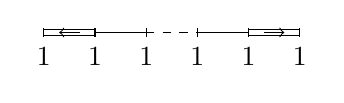
\begin{tikzpicture}[x=.65cm,y=.6cm]
\draw(0,.06)--(1,.06) (0,-.06)--(1,-.06);\draw[->](.7,0)--(.3,0);
\draw(1,0)--(2,0);\draw[dashed](2,0)--(3,0);\draw(3,0)--(4,0);
\draw(4,.06)--(5,.06) (4,-.06)--(5,-.06);\draw[->](4.3,0)--(4.7,0);
\foreach \x in {0,...,5}{\draw(\x,-.09)--(\x,.09);\node[below]at(\x,-.12){$1$};}
\end{tikzpicture}
\end{center}
特殊顶点为图的两个端点，它们不对应超特殊点。注意，在非分歧情形，Weyl 群 $W$ 为 $B_n$ 型仿射反射群；在分歧情形，则为 $C_n$ 型。
\origsection{2}{建筑（The building）}
\origsubsection{2.1}{定义（Definitions）}
$G$ 在 $K$ 上的建筑（building）$\mathscr B=\mathscr B(G,K)$ 可将 $G$ 的各个极大 $K$ 分裂环面的公寓粘合起来构造。更确切地，下述陈述给出 $\mathscr B$ 的一个定义；其中“$G(K)$ 集”指带 $G(K)$ 左作用的集合。

设 $A=A(G,S,K)$ 如 1.2。则在唯一同构意义下，存在唯一的包含 $A$ 的 $G(K)$ 集 $\mathscr B$，具有下述性质：$\mathscr B=\bigcup_{g\in G(K)}gA$；群 $N(K)$ 保持 $A$，并通过 $\nu$ 在其上作用（见 1.2）；对每个仿射根 $\alpha$，1.4 的群 $X_\alpha$ 逐点固定半公寓 $A_\alpha=\alpha^{-1}([0,\infty))$。

（注意：建筑 $\mathscr B$ 的“典范性”与 $A$ 相同，见 1.2。）

证明大致如下。假设 $G$ 半单（这一步不损失问题的本质）。在承认 1.4.1 和 1.4.2 的条件下，正如 1.5 所解释，[8，7.4] 证明了 $\mathscr B$ 的存在。于是显然存在具有所给性质的“泛”$G(K)$ 集 $\overline{\mathscr B}$，它由直积 $G(K)\times A$ 对某个等价关系取商得到。$\overline{\mathscr B}$ 到 [8，7.4.2] 定义的建筑 $\mathscr I$ 的典范映射显然满射，它也为单射，因为容易验证，$\overline{\mathscr B}$ 的一个点的稳定子包含其在 $\mathscr I$ 中的像的稳定子。因此，$\mathscr I$ 满射到任意具有所需性质的 $G(K)$ 集 $\mathscr B$；利用 [8，7.3.4] 可证明，$A$ 的点在 $\mathscr B$ 中的稳定子不能比在 $\mathscr I$ 中更大，否则它与 $N(K)$ 的交会超过规定的 $N(K)$ 在 $A$ 上的作用所允许的范围。

集合 $gA$，$g\in G(K)$，称为建筑的公寓。公寓 $gA$ 可自然等同于极大分裂环面 $\prescript{g}{}{S}$ 对应的公寓。这给出 $\mathscr B$ 的公寓与 $G$ 的极大 $K$ 分裂环面之间的一一对应：事实上，$gA$ 是被 $\prescript{g}{}{S}(K)$ 保持的唯一公寓（[8，2.8.11] 的证明说明这一点），而确定 $\prescript{g}{}{S}$ 的 $\prescript{g}{}{N}(K)$ 是 $gA$ 在 $G(K)$ 中的稳定子。“在多数情形下”，$gA$ 还可刻画为单位群
\[
\prescript{g}{}{S}^\circ=\{s\in\prescript{g}{}{S}(K)\mid\omega(\chi(s))=0\text{ 对所有 }\chi\in X^*(\prescript{g}{}{S})\}
\]
在 $\mathscr B$ 中的不动点集，但这并不总成立（更精确的陈述见 3.6）。

还需注意，半公寓 $A_\alpha$（$\alpha\in\Phi_{\mathrm{af}}$）从来不是群 $X_\alpha$ 的不动点集。事实上，若按下文 2.3 赋予 $\mathscr B$ 度量，则存在常数 $c$，使对 $A_\alpha$ 中距墙 $\partial A_\alpha$ 的距离为 $d$ 的每个点 $x$，整个以 $x$ 为中心、半径为 $cd$ 的球均被 $X_\alpha$ 逐点固定（见 [8，7.4.33]）。

如果 $S_1$ 为 $G^\circ$ 的中心的极大分裂环面，$G_1,\ldots,G_m$ 为 $G^\circ$ 的近单因子（almost simple factors），则建筑 $\mathscr B$ 典范同构于各建筑 $\mathscr B(S_1,K)$（它是仿射空间）与 $\mathscr B(G_i,K)$，$i=1,\ldots,m$，的直积。如果 $G$ 在 $K$ 上各向异性，即 $S=\{1\}$，则 $\mathscr B$ 只有一个点。如果 $G=R_{L/K}H$，其中 $L/K$ 可分、$H$ 为 $L$ 上约化群，则建筑 $\mathscr B(G,K)$ 与 $\mathscr B(H,L)$ 典范同构。
\origsubsection{2.2}{建筑上的仿射结构、面、收缩、拓扑及其他典范结构（Affine structures, facets, retractions, topology and other canonical structures）}
由于 $A$ 在 $G(K)$ 中的稳定子 $N(K)$ 保持其仿射结构及分面的划分，$\mathscr B$ 的每个公寓 $gA$，$g\in G(K)$，都自然带有实仿射空间结构与分面的划分。这些结构在交集上一致。事实上，

\paragraph*{2.2.1.}若 $A',A''$ 为两个公寓，则存在 $G(K)$ 的元素，将 $A'$ 映至 $A''$，并逐点固定交集 $A'\cap A''$；此外，$A'\cap A''$ 是 $A'$ 中若干面的闭凸并集（因此在 $A''$ 中也是如此）[8，7.4.8]。

由此得到 $\mathscr B$ 的分面划分，其中在公寓中为开集的面称为室。特别地，如果 $G^\circ$ 拟单（半单），则 $\mathscr B$ 是单纯（多单纯）复形（simplicial/polysimplicial complex）。

给定 $\mathscr B$ 的两个面，存在同时包含它们的公寓 [8，7.4.18]。特别地，给定 $x,y\in\mathscr B$，存在包含它们的公寓。由 2.2.1，对 $t\in[0,1]\subset\R$，在这样的公寓中定义的点 $(1-t)x+ty$ 与公寓的选择无关。集合 $\{(1-t)x+ty\mid t\in[0,1]\}$ 称为 $\mathscr B$ 中连接 $x,y$ 的测地线段（geodesic segment）。

设 $A'$ 为一个公寓，$C\subset A'$ 为一个室。对每个包含 $C$ 的公寓，存在从该公寓到 $A'$ 的唯一逐点固定 $C$ 的仿射空间同构。由 2.2.1，这些同构可粘合成映射 $\rho_{A';C}:\mathscr B\to A'$，称为以 $C$ 为中心、从 $\mathscr B$ 到 $A'$ 的收缩（retraction）。显然，$\rho_{A';C}$ 将测地线段映为折线，即有限条测地线段的连通并。

通常在建筑 $\mathscr B$ 上赋予一个 $G(K)$ 不变拓扑，最自然的定义借助下文 2.3 的度量；也可更典范地定义为使所有 $\rho_{A';C}$ 连续的最弱拓扑。如果剩余域 $\overline K$ 有限，此拓扑使 $\mathscr B$ 成为局部紧空间，且与“CW 拓扑”一致，即全部公寓不交并上自然拓扑的商拓扑。否则，它严格弱于后者。无论何种情形，拓扑空间 $\mathscr B$ 均可缩（contractible）。事实上，对每个点 $x\in\mathscr B$，由 $\varphi_t(y)=tx+(1-t)y$ 定义的映射 $\varphi_t:\mathscr B\to\mathscr B$，构成从恒等映射到 $\mathscr B$ 至 $\{x\}$ 的收缩的同伦（homotopy）[8，7.4.20]。

如果 $\mathscr B$ 的一个子集在某个收缩 $\rho_{A';C}$ 下的像有界，则称其有界（bounded）；容易看出，此时它在每个这种收缩下的像均有界。按通常的定义，若对 $G$ 上每个 $K$ 正则函数 $f$，集合 $\omega(f(H))$ 都有下界，就称 $G(K)$ 的子集 $H$ 有界。$G(K)$ 在 $\mathscr B$ 上的作用在下述意义下有界且“适当”（proper）：映射 $(g,b)\mapsto(gb,b)$，从 $G(K)\times\mathscr B$ 到 $\mathscr B\times\mathscr B$，将有界子集（即有界集的乘积的子集）映为有界集，而且 $\mathscr B\times\mathscr B$ 中有界子集的原像有界。若 $\overline K$ 有限，“有界”与“相对紧”同义；特别地，$G(K)$ 在 $\mathscr B$ 上的作用在通常意义下适当。
\origsubsection{2.3}{度量与单纯形分解（Metric and simplicial decomposition）}
在各种问题中，建筑对于 $p$ 进约化群所起的作用，类似于对称空间（symmetric spaces）在非紧实单 Lie 群研究中所起的作用（见 [24，第 5 节] 及其中的参考文献）。本节说明这种类比的若干方面；另参见 [18，5.32]。注意，与 2.2 引入的结构不同，这里考虑的结构至少在 $G$ 不半单时并非典范。

在 $V$ 中选取一个 Weyl 群 $\prescript{v}{}{W}$ 不变的内积。如果 $G$ 拟单，此内积在差一个标量因子的意义下唯一，且有各种“自然”的正规化方法（Killing 型、规定短余根长度等）。$G$ 半单时，也可逐分支作典范选择；一般情形则不行。由该内积得到 $A$ 上的 Euclidean 距离，再通过 $G(K)$ 的作用得到任一公寓上的距离。由 2.2.1，$\mathscr B$ 的两点 $x,y$ 在包含它们的所有公寓中有相同距离 $d(x,y)$。2.2 中收缩 $\rho_{A';C}$ 的性质容易推出：赋予距离函数 $d:\mathscr B\times\mathscr B\to\R_+$ 后，建筑 $\mathscr B$ 是完备度量空间（complete metric space）[8，2.5]。对应拓扑与 2.2 定义的相同。再次利用收缩，可证明 [8，3.2.1]：若 $x,y,z,m\in\mathscr B$ 且 $d(x,m)=d(y,m)=\frac12d(x,y)$，则
\[
d(x,z)^2+d(y,z)^2\geq2d(m,z)^2+\tfrac12d(x,y)^2.
\]
在 Riemann 几何中，此不等式刻画截面曲率（sectional curvature）为负的空间（因而在非紧不可约对称空间中成立）。\footnote{\textbf{译者注（本次校订）：}这里应为截面曲率“非正”，而非“为负”。在完备、单连通的 Riemann 流形中，所示中点不等式对应非正曲率；高秩非紧对称空间包含二维平坦子空间，其截面曲率可以为零。}与 Riemann 情形类似，这里可用它证明下面的不动点定理。

\paragraph*{2.3.1.}$\mathscr B$ 的等距变换（isometries）的一个有界群必有不动点 [8，3.2.4]。有趣的应用来自 Galois 群（建筑的“Galois 下降”，Galois descent）及 $G(K)$ 的有界子群（见 3.2）。

某些应用中（例如 [2]），需要 $\mathscr B$ 的一个 $G(K)$ 不变单纯形分解。只需选取 $A$ 的一个 $N(K)$ 不变、比按面划分更细的单纯形分解（容易看出这种分解总存在），并通过 $G(K)$ 作用搬移到全部公寓。如果 $G$ 半单，可更直接地使用多单纯面划分的典范重心细分（barycentric subdivision）。如果 $G$ 拟单，该划分本身就满足要求。
\origsubsection{2.4}{Dynkin 图；特殊点与超特殊点（Dynkin diagram; special and hyperspecial points）}
设 $C$ 为 $\mathscr B$ 的一个室。从包含 $C$ 的任一公寓出发，可依 1.8 定义局部 Dynkin 图 $\Delta(G,C)$；由 2.2.1，它在唯一同构意义下与公寓选择无关。如果 $C'$ 为另一个室，将 1.8.1 用于同时包含 $C,C'$ 的任一公寓，得到同构 $\varphi_{C'C}:\Delta(G,C)\to\Delta(G,C')$，由 2.2.1，它仍与公寓无关。所有这些同构相容：若 $C,C',C''$ 为三个室，则 $\varphi_{C''C}=\varphi_{C''C'}\circ\varphi_{C'C}$。因此，可以谈论 $G$ 在 $K$ 上的局部 Dynkin 图 $\Delta(G)=\Delta(G,K)$，它在唯一同构意义下良定义。绝对局部 Dynkin 图（1.11）、局部指标（1.11）亦然；前者正是 $G$ 在 $K$ 的非分歧闭包 $K_1$ 上的图 $\Delta(G,K_1)$。

1.9 和 1.10 的定义立即推广至建筑 $\mathscr B$ 的任意点 $x$、任意面 $F$：选取包含 $x$ 或 $F$ 的公寓，采用相应定义，再由 2.2.1 得到结果与公寓选择无关。因此，$\mathscr B$ 的每个点 $x$（面 $F$）都典范地对应于 $\Delta(G)$ 的一个顶点集 $I_x$（$I_F$），以及根系 $\Phi_x$（$\Phi_F$）；后者仅在非典范同构意义下定义。也可谈论 $\mathscr B$ 的特殊点与超特殊点。1.9 最后一段用 $I_x$ 判别特殊点的准则当然仍成立。超特殊点存在的必要条件是 $G$ 在 $K$ 的某个非分歧扩张上分裂；若 $G$ 拟分裂，这一条件也充分。

图 $\Delta(G)$ 的每个顶点 $v$ 都带一个整数 $d(v)$。1.8 中的定义借助公寓 $A$，但仍由 2.2.1，结果与其选择无关。如果剩余域 $\overline K$ 有限，同构于 $\F_q$，则 $d(v)$ 可解释如下：“类型为 $v$”的余维一的面 $F$，即 $I_F$ 为 $\Delta(G)$ 全部顶点集去掉 $v$ 后的补集，恰被 $q^{d(v)}+1$ 个室的闭包包含（见 3.5）。
\origsubsection{2.5}{自同构的作用；特殊点与超特殊点的共轭类（Action of automorphisms; conjugacy classes of special and hyperspecial points）}
$G$ 的全部 $K$ 自同构组成的群 $(\Aut G)(K)$，特别是 $G^\circ$ 的伴随群 $G_{\mathrm{ad}}$ 的有理点群 $G_{\mathrm{ad}}(K)$，通过结构搬移作用于 $\mathscr B$ 与局部 Dynkin 图 $\Delta=\Delta(G)$。通过典范同态 $\operatorname{int}:G\to\Aut G$，得到 $G(K)$ 在 $\mathscr B$ 与 $\Delta$ 上的作用。由 $\mathscr B$ 作为 $G(K)$ 集的定义所给出的 $G(K)$ 在 $\mathscr B$ 上的作用，在 $G$ 半单时与此作用一致，一般时不然；但两者在 $\Delta$ 上诱导的作用总相同。记 $\Xi=\Xi(G,K)$ 为 $G(K)$ 在 $\Aut\Delta$ 中的像。

如果 $G$ 半单且单连通，它在 $\Delta$ 上的作用平凡，即 $\Xi=\{1\}$（这是 1.13 所述现象的又一体现）。

假设 $G$ 连通。则 $\Xi$ 也是 $Z(K)$ 在 $\Aut\Delta$ 中的像，计算如下：以 $\widetilde G$ 表示 $G$ 导群的单连通覆盖，以 $\widetilde S$ 表示 $\widetilde G$ 中其在 $G$ 中的像包含于 $S$ 的极大分裂环面，以 $\widetilde Z$ 表示 $\widetilde S$ 在 $\widetilde G$ 中的中心化子，以 $S_1$ 表示 $S$ 中在 $G$ 内中心的极大子环面，以 $Z_s$ 表示 $\widetilde Z(K)$ 在 $Z(K)$ 中的像。则 $S_1(K)$、$Z_s$ 以及 $Z_c=\{z\in Z(K)\mid\omega(\chi(z))=0\text{ 对所有 }\chi\in X^*(Z)\}$（见 1.2）均为 $Z(K)$ 的正规子群，乘积 $S_1(K)Z_sZ_c$ 是 $Z(K)$ 在 $\Delta$ 上作用的核。因此
\[
\Xi=Z(K)/(S_1(K)\cdot Z_s\cdot Z_c).
\]
若 $G$ 拟分裂，特别是 $\overline K$ 代数闭时，$Z,\widetilde Z$ 是环面，计算 $\Xi$ 尤为简单。注意，在多数常见情形中，$\Aut\Delta$ 的子群 $\Xi$ 由其底层“抽象”群唯一确定。

$\mathscr B$ 的两个面 $F,F'$ 位于同一个 $G(K)$ 轨道中（对上述两种 $G(K)$ 作用均如此），当且仅当 $I_F,I_{F'}$（见 2.4）位于同一个 $\Xi$ 轨道。特别地，若 $G$ 半单且单连通，则 $G(K)$ 在 $\mathscr B$ 的特殊点集中的轨道，与从 $\Delta$ 每个连通分支各取一个特殊顶点所成的顶点集，典范地一一对应。

假设 $G$ 半单。若 $G$ 在 $K$ 上分裂，则 $G_{\mathrm{ad}}(K)$ 传递地置换 $\mathscr B$ 的特殊点，这是 [5，VI.2.2，命题 2] 的直接推论。逐情形分析表明，对任意半单 $G$，$G_{\mathrm{ad}}(K)$ 都传递地置换特殊点；可能的例外只在 $\Delta$ 的底层 Coxeter 图存在形如下图的连通分支时：
\begin{center}
\begin{tikzpicture}[x=.6cm,y=.6cm]
\draw(0,.07)--(1,.07) (0,-.07)--(1,-.07) (1,0)--(2,0);\draw[dashed](2,0)--(3,0);\draw(3,0)--(4,0) (4,.07)--(5,.07) (4,-.07)--(5,-.07);
\foreach \x in {0,1,2,3,4,5}{\draw(\x,-.1)--(\x,.1);}
\node[above]at(0,.15){s};\node[above]at(5,.15){s};\node at(6,0){或};\draw[line width=2pt](7,0)--(8,0);\node[above]at(7,.15){s};\node[above]at(8,.15){s};
\end{tikzpicture}
\end{center}
现假设 $G$ 拟单，且上述 Coxeter 图是这些图之一。$G_{\mathrm{ad}}(K)$（甚至 $(\Aut G)(K)$）传递地置换特殊点的显然必要条件，是存在置换其两个特殊顶点的 $\Delta$ 自同构，且它们所带的 $d(v)$ 相等。可验证，若剩余域 $\overline K$ 有限，这些条件也充分。

对任意 $G$，若 $\mathscr B$ 有超特殊点，则由这种点构成的面被 $G_{\mathrm{ad}}(K)$ 传递地置换；因而 $G$ 半单时，这些点本身被传递地置换。
\origsubsection{2.6}{域扩张下的行为（Behaviour under field extensions）}
建筑关于 Galois 扩张具有函子性。

更确切地，对 $K$ 的每个 Galois 扩张 $K_1$，可考虑建筑 $\mathscr B(G,K_1)$，Galois 群 $\Gal(K_1/K)$ 在其上自然作用（非半单情形须按 1.2 使公寓、从而使 $\mathscr B$ 典范化）。存在唯一的单射系统
\[
\iota_{K_2K_1}:\mathscr B(G,K_1)\longrightarrow\mathscr B(G,K_2),
\qquad K_1\subset K_2,\quad K_1,K_2\text{ 为 }K\text{ 的 Galois 扩张},
\]
满足：$\iota_{K_2K_1}$ 的像被 $\Gal(K_2/K_1)$ 逐点固定；$\iota_{K_2K_1}$ 在 $\mathscr B(G,K_1)$ 的任一公寓上的限制，是映入 $\mathscr B(G,K_2)$ 的某个公寓的仿射映射；$\iota_{K_2K_1}$ 是 $G(K_1)$ 等变的（covariant）；若 $K_1\subset K_2\subset K_3$，则 $\iota_{K_3K_1}=\iota_{K_3K_2}\circ\iota_{K_2K_1}$。最后一个性质使我们能相容地将每个 $\mathscr B(G,K_1)$ 与它在每个 $\iota_{K_2K_1}$ 下的像等同。

\paragraph*{2.6.1.}若 $K_1/K$ 非分歧（甚至驯分歧，见 [19]），则 $\mathscr B$ 是 $\Gal(K_1/K)$ 在 $\mathscr B(G,K_1)$ 中的不动点集；公寓 $A=A(G,S,K)$ 是 $\mathscr B$ 与任一包含 $S$ 的极大 $K_1$ 分裂 $K$ 环面 $S_1$ 的公寓 $A(G,S_1,K_1)$ 的交。仍假设 $K_1/K$ 非分歧，由 1.10.2，$\mathscr B$ 中在 $\mathscr B(G,K_1)$ 内特殊的点 $x$，在 $\mathscr B$ 中也特殊；若进一步 $G$ 在 $K_1$ 上分裂，则 $x$ 超特殊。

若 $K_1/K$ 野分歧（wildly ramified），$\Gal(K_1/K)$ 在 $\mathscr B(G,K_1)$ 中的不动点集可能严格大于 $\mathscr B$，其形状仿佛是在建筑 $\mathscr B$ 周围多长出了一些分支。例如，设 $G$ 分裂且不是环面，$K=\Q_2$，$K_1/K$ 完全分歧且 $K_1\ne K$（这蕴涵 $K_1/K$ 野分歧）。$\mathscr B$ 的公寓 $A=A(G,S,K)$ 也是 $\mathscr B(G,K_1)$ 的一个公寓。取 $A$ 中相对于 $K_1$ 的余维一的面 $F$，使它不是相对于 $K$ 的面（见 1.10.1 后的例子）。由 1.8 和 2.4 的最后断言，$\mathscr B(G,K_1)$ 中恰有一个不包含于 $A$、闭包包含 $F$ 的室；它当然被 $\Gal(K_1/K)$ 固定，且不可能包含于 $\mathscr B$，因为 $F$ 不是 $\mathscr B$ 的面。

上述结果的证明及更详细的分析见 [19]。
\origsubsection{2.7}{例：相对秩为一的群（Example: groups of relative rank 1）}
相对秩为一的半单群的建筑是维数为一的可缩单纯复形，即一棵树（tree）。它的全部顶点均为特殊点。如果 $\overline K\simeq\F_q$，$d,d'$ 为 Dynkin 图的两个顶点所带的整数 $d(v)$，则树的每条边的一个顶点的度为 $q^d+1$，另一个顶点的度为 $q^{d'}+1$（见 2.4）。例如，取 $\Q_2$ 上五个变量的一个非分裂二次型的特殊正交群，此时 $d=1$、$d'=2$，其建筑如图所示。此时度为 $5$ 的顶点超特殊，其余顶点不是。\footnote{\textbf{译者注（本次校订）：}对这里的非分裂五维二次型，最后一句中的“超特殊”不成立。它的特殊正交群是分裂 $\operatorname{SO}_5$ 的非拟分裂内形式；有限剩余域上，具有超特殊点的约化群必为拟分裂群。此例的顶点均为特殊点，但均非超特殊点，度数差异本身不能判定超特殊性。}
\begin{center}\begin{tikzpicture}[line width=.4pt,scale=1.1]
\coordinate (o)at(0,0);
\foreach \a in {90,210,330}{
\coordinate(a\a)at(\a:1);\draw(o)--(a\a);
\foreach \b in {-45,-15,15,45}{
\pgfmathsetmacro{\ang}{\a+\b}
\coordinate(b\a\b)at($(a\a)+(\ang:.62)$);\draw(a\a)--(b\a\b);
\foreach \c in {-16,16}{\pgfmathsetmacro{\angtwo}{\ang+\c}\coordinate(c\a\b\c)at($(b\a\b)+(\angtwo:.35)$);\draw(b\a\b)--(c\a\b\c);
\foreach \d in {-24,-8,8,24}{\pgfmathsetmacro{\angthree}{\angtwo+\d}\draw[densely dotted](c\a\b\c)--++(\angthree:.22);}
}
}
}
\end{tikzpicture}
\end{center}
\origsubsection{2.8}{例：$\SL_3$ 与 $\GL_3$（Example: $\SL_3$ and $\GL_3$）}
假设 $G=\SL_3$。建筑 $\mathscr B=\mathscr B(G,K)$ 是二维单纯复形，对 2.3 引入的度量，其极大单纯形是等边三角形。公寓为按熟知方式剖分成三角形的 Euclidean 平面：
\begin{center}
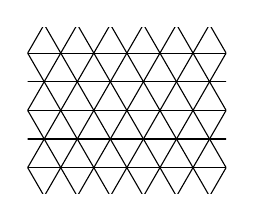
\begin{tikzpicture}[scale=.42]
\clip(-3,-2.5)rectangle(3,2.5);
\foreach \k in {-6,...,6}{\draw(-6,{.8660254*\k})--(6,{.8660254*\k});\draw({\k-3},-5.196152)--({\k+3},5.196152);\draw({\k+3},-5.196152)--({\k-3},5.196152);}
\end{tikzpicture}
\end{center}
整个建筑则沿每条边分叉；若 $q=\operatorname{card}\overline K$，则每条边属于 $q+1$ 个三角形。$\mathscr B$ 每个顶点的链环（link），是 $\SL_3(\overline K)$ 的“球面建筑”（spherical building），即 $\overline K$ 上某射影平面的“旗复形”（flag complex）；$\overline K\simeq\F_2$ 的特殊情形的图见 [24] 或 [26]。$\mathscr B$ 的全部顶点均超特殊。

建筑 $\mathscr B(\GL_3,K)$ 是 $\mathscr B$ 与一条仿射直线的直积。
\origsubsection{2.9}{例：一般线性群（Example: general linear groups）}
采用 1.14 的假设与记号。特别地，$D$ 为 $K$ 上的有限维中心除代数，$G=\GL_{n,D}$（所以 $G(K)=\GL_n(D)$）。则建筑 $\mathscr B=\mathscr B(G,K)$ 可解释为 $D^n$ 上全部“加性范数”（additive norms）的集合 $\mathcal N$，即所有满足
\[
\begin{aligned}
\varphi(x+y)&\geq\inf\{\varphi(x),\varphi(y)\},&&x,y\in D^n,\\
\varphi(xd)&=\varphi(x)+\omega(d),&&x\in D^n,\ d\in D
\end{aligned}
\]
的函数 $\varphi:D^n\to\R\cup\{+\infty\}$。\footnote{\textbf{译者注（本次校订）：}加性范数还须满足 $\varphi(x)=+\infty$ 当且仅当 $x=0$。仅靠上列两条关系，恒等于 $+\infty$ 的函数也会被纳入，而它不对应建筑中的点。}

更确切地，如 1.14 将公寓 $A$ 与 $V$ 等同，则将 $\sum_{i=1}^nv_ie_i$ 映为范数
\[
(x_1,\ldots,x_n)\longmapsto\inf\{\omega(x_i)-v_i\mid i=1,\ldots,n\}
\]
的映射 $A\to\mathcal N$，可唯一延拓为 $G(K)$ 集的同构 $\mathscr B\to\mathcal N$，其中 $G(K)$ 通过 $(g\varphi)(x)=\varphi(g^{-1}x)$ 作用于 $\mathcal N$。范数 $\varphi$ 特殊，即对应于 $\mathscr B$ 的特殊点，当且仅当存在向量空间 $D^n$ 的一组基 $(b_i)_{1\leq i\leq n}$ 及实数 $f$，使
\[
\varphi\left(\sum_{i=1}^nb_id_i\right)=f+\inf\{\omega(d_i)\mid i=1,\ldots,n\},\qquad d_i\in D.
\]
$\varphi$ 超特殊，当且仅当它特殊且 $D=K$。

$\mathscr B(\SL_{n,D},K)$ 的类似解释见 [8，第 238 页]。空间 $\mathcal N$ 最早由 O. Goldman 与 N. Iwahori [12] 考虑。
\origsubsection{2.10}{例：特殊酉群（Example: special unitary groups）}
$L,\omega,\pi_1,\Gamma_1,\tau,\delta$ 的含义同 1.15。特别地，$L/K$ 为可分二次扩张，且 $\delta=\sup\{\omega(d)\mid d\in L,d+d^\tau=1\}$。设 $E$ 为带有关于 $\tau$ 的非退化 Hermite 型 $h$ 的有限维 $L$ 向量空间，$G=\operatorname{SU}(h)$。则 $G$ 在 $K$ 上的建筑 $\mathscr B$（这也就是 $U(h)$ 的建筑），可解释为全部满足不等式
\[
\begin{aligned}
\omega(h(x,x))&\geq2\varphi(x)-\delta,&&x\in E,\\
\omega(h(x,y))&\geq\varphi(x)+\varphi(y),&&x,y\in E,
\end{aligned}
\]
且在逐点比较的偏序下为极大的加性范数 $\varphi:E\to\R\cup\{+\infty\}$ 的集合 $\mathcal N_h$（更一般的结果见 [8，第 239 页]）。

再假设 $E=L^{2n+1}$，且 $h$ 如 1.15（1）。$\mathscr B$ 与 $\mathcal N_h$ 的等同可更具体地描述：沿用 1.15 的记号，将 $\sum_{i=1}^nv_ie_i$ 映为范数\nobreak\footnote{\textbf{译者注（本次校订）：}本节两处显式范数中的中间坐标项应为 $\omega(x_0)+\delta/2$，而非 $\omega(x_0)-\delta$。取 $x=b_0$，则 $h(b_0,b_0)=1$，上面的第一条不等式给出 $\varphi(b_0)\le\delta/2$，极大范数取等号；原式在 $\delta<0$ 时已经违反该不等式。另外，式2.10(1)左边的求和应遍历 $-n\le i\le n$，以包括负指标和零指标。}
\[
(x_{-n},\ldots,x_n)\longmapsto
\inf\{\omega(x_i)-v_i,\omega(x_{-i})+v_i,\omega(x_0)-\delta\mid1\leq i\leq n\}
\]
的映射 $A\to\mathcal N_h$，唯一延拓为 $G(K)$ 集的同构 $\mathscr B\to\mathcal N_h$。范数 $\varphi\in\mathcal N_h$ 特殊，即对应 $\mathscr B$ 的特殊点，当且仅当存在 $E$ 的一组基 $(b_i)$，使 $h$ 关于此基为 1.15（1）的形式，且存在常数 $f\in\frac12\Gamma_1$，使对 $x_i\in L$，有
\[
\varphi\left(\sum_{i=1}^nb_ix_i\right)=
\inf\{\omega(x_i)-f,\omega(x_{-i})+f,\omega(x_0)-\delta\mid1\leq i\leq n\}.\tag{2.10(1)}
\]
这时可选基 $(b_i)$ 使 $f=0$ 或 $\frac12\omega(\pi_1)$。若 $L/K$ 非分歧且存在 $E$ 的基 $(b_i)$，使（1）在 $f=0$ 时成立，则范数 $\varphi$ 超特殊。

\origsection{3}{稳定子与中心化子（Stabilizers and centralizers）}
从现在起，假设 $G$ 连通。
\origsubsection{3.1}{记号；一个 BN 对（Notations; a BN-pair）}
对 $K$ 的每个分歧指数有限的代数扩张 $K_1$，以及建筑 $\mathscr B(G,K_1)$ 的每个子集 $\Omega$，以 $G(K_1)^\Omega$ 表示 $G(K_1)$ 中逐点固定 $\Omega$ 的全部元素组成的群。如果 $\Omega$ 只有一个点 $x$，也将 $G(K_1)^\Omega$ 写作 $G(K_1)^x$。注意，若 $F$ 是 $\mathscr B(G,K_1)$ 的面，$x$ 是 $F$ 中处于“一般位置”的点，则 $G(K_1)^F=G(K_1)^x$。特殊点（超特殊点）$x\in\mathscr B$ 的稳定子 $G(K)^x$ 称为 $G(K)$ 的特殊子群（special subgroups）（超特殊子群，hyperspecial subgroups）。

回顾，如果 $G$ 半单且单连通，则群 $\widetilde W=N(K)/Z(K)$ 与仿射根系 $\Phi_{\mathrm{af}}$ 的 Weyl 群 $W$ 一致。仍令 $\mathscr B=\mathscr B(G,K)$。\footnote{\textbf{译者注（本次校订）：}此处应沿用 $\widetilde W=N(K)/Z_c$；见1.13的校订注。}

\paragraph*{3.1.1.}假设 $\widetilde W=W$。则对 $\mathscr B$ 的每个面 $F$ 及每个 $x\in F$，有 $G(K)^F=G(K)^x$。此外，若 $C$ 为 $A=A(G,S)$ 的室，则 $(G(K)^C,N(K))$ 是 $G(K)$ 中 Weyl 群为 $W$ 的 BN 对（也称 Tits 系统，Tits system，见 [5]、[23]）。这时群 $G(K)^x$，$x\in\mathscr B$，称为 $G(K)$ 的旁抛物子群（parahoric subgroups）（见 [8]）；不过本文避免使用这一术语，以免预先决定它向非单连通情形的最佳推广。上述 BN 对还给出另一种构造建筑 $\mathscr B$ 的方法：先独立地定义 BN 对，再借助它定义旁抛物子群并构造建筑；详见 [8，第 2 节]。

设 $\Omega$ 为公寓 $A$ 的非空子集，其到 $G$ 的半单部分的建筑的投影（见 2.1 最后一段）有界。对任一根 $a\in\Phi$，以 $\alpha(a,\Omega)$ 表示向量部分为 $a$ 且在 $\Omega$ 上为正的最小仿射根。\footnote{\textbf{译者注（本次校订）：}此处“为正”须理解为“非负”。若 $\Omega$ 位于某一墙上，定义其逐点稳定子时必须保留在该墙上取零值的仿射根子群；严格正性会漏掉这些子群。}令 $\Phi'$ 为所有不可除根（nondivisible roots）的集合，即满足 $\frac12a\notin\Phi$ 的根 $a\in\Phi$；任意选取 $\Phi$ 的一组基，以 $\Phi'^+$、$\Phi'^-$ 分别表示关于此基为正、为负的不可除根集合。令 $N(K)^\Omega=N(K)\cap G(K)^\Omega$，$Z_c,X_\alpha$ 如 1.2、1.4 定义。则有如下 $G(K)^\Omega$ 的群论描述（见 [8，6.4.9、6.4.48、7.4.4]）：

若 $X^\pm(\Omega)$ 为所有 $a\in\Phi'^\pm$ 的 $X_{\alpha(a,\Omega)}$ 生成的群，则乘积映射
\[
\prod_{a\in\Phi'^\pm}X_{\alpha(a,\Omega)}\longrightarrow X^\pm(\Omega)
\]
无论怎样排列因子都是双射，且
\[
G(K)^\Omega=X^-(\Omega)\cdot X^+(\Omega)\cdot N(K)^\Omega.
\]
若 $\Omega$ 包含 $A$ 的开子集，则乘积映射
\[
\prod_{a\in\Phi'}X_{\alpha(a,\Omega)}\times Z_c\longrightarrow G(K)^\Omega
\]
无论怎样排列因子都是双射。
\origsubsection{3.2}{极大有界子群（Maximal bounded subgroup）}
对 $\mathscr B$ 的每个非空子集 $\Omega$，$G(K)^\Omega$ 是 $G(K)$ 的有界子群（见 2.2）。若剩余域 $\overline K$ 有限，$G(K)^\Omega$ 甚至为紧群，且下文“极大有界”可换成“极大紧”。

由 2.3.1 容易推出：$G(K)$ 的每个有界子群均包含于某个极大有界子群，每个极大有界子群均为 $\mathscr B$ 的某点 $x$ 的稳定子 $G(K)^x$。

进一步，若 $x$ 属于 $\mathscr B$ 的最小维数的面，则 $G(K)^x$ 是 $G(K)$ 的极大有界子群；特别地，特殊子群均为极大有界子群。由 3.1.1，上述两个陈述给出单连通情形极大有界子群的完整描述：

若 $G$ 半单且单连通，则 $G(K)$ 的极大有界子群恰为建筑 $\mathscr B$ 的顶点的稳定子；它们形成 $\prod_{i=1}^r(l_i+1)$ 个共轭类，其中 $l_1,\ldots,l_r$ 是 $G$ 的各拟单因子的相对秩。

非单连通情形的分析见 [8，3.3.5]。
\origsubsection{3.3}{各种分解（Various decompositions）}
设 $C$ 为 $A=A(G,S)$ 的一个室。将 $A$ 与向量空间 $V$ 等同，使 $0$ 成为包含于 $C$ 的闭包的特殊点；特别地，$G(K)^0$ 是 $G(K)$ 的特殊子群。令 $D=\R_+^*\cdot C$（一个“向量室”，vector chamber），$B=G(K)^C$。若 $\overline K$ 有限，更一般地，若 $G$ 剩余拟分裂且单连通，则 $B$ 为 $G(K)$ 的 Iwahori 子群（见 3.7）。令 $U^+$ 为所有 $a|_C$（因而 $a|_D$）为正的 $U_a$ 生成的群，以 $Y$ 表示“$V$ 与 $\widetilde W$ 的交”，即 $\widetilde W$ 中 $A$ 的全部平移组成的群；因此 $Y$ 是 $Z(K)$ 在 1.2 的同态 $\nu$ 下的像。令 $Y_+=Y\cap\overline D$（$D$ 的闭包），$Z(K)_+=\nu^{-1}(Y_+)$，后者为 $Z(K)$ 的子半群。

\paragraph*{3.3.1. Bruhat 分解（Bruhat decomposition）}有 $G(K)=BN(K)B$，且映射 $BnB\mapsto\nu(n)$，$n\in N(K)$，是从集合 $\{BgB\mid g\in G(K)\}$ 到 $\widetilde W$ 的双射。

若 $n\in N(K)$、$\nu(n)=w$，如常写 $BnB=BwB$。若 $\overline K=\F_q$，$BwB/B$ 的基数 $q_w$（例如在 [1] 中使用）可用 1.8 的整数 $d(v)$ 按下式给出：写 $w=r_1\cdots r_lw_0$，其中 $(r_1,\ldots,r_l)$ 是 Coxeter 群 $W$ 的一个既约词，$w_0(C)=C$；令 $v_i$ 为 $\Delta$ 中代表 $r_i$ 的顶点。则 $q_w=q^d$，$d=\sum_{i=1}^ld(v_i)$。特别地，$d(v)$ 有另一解释：$q^{d(v)}=q_{r(v)}$，其中 $r(v)$ 为 $\Delta$ 的顶点 $v$ 对应的基本反射。

更一般地，对任意 $\overline K$，商 $BwB/B$ 自然具有 $\overline K$ 上的“完全簇”（perfect variety）结构，按 Serre 的定义，见 Publ. Math. I.H.E.S. 7 (1960)，1.4；沿用上述记号，作为这种簇，它同构于维数为 $\sum_{i=1}^ld(v_i)$ 的 $\overline K$ 向量空间。

\paragraph*{3.3.2. Iwasawa 分解（Iwasawa decomposition）}有 $G(K)=G(K)^0Z(K)U^+(K)$，且映射 $G(K)^0zU^+(K)\mapsto\nu(z)$，$z\in Z(K)$，是从集合 $\{G(K)^0gU^+(K)\mid g\in G(K)\}$ 到 $Y$ 的双射。

\paragraph*{3.3.3. Cartan 分解（Cartan decomposition）}有 $G(K)=G(K)^0Z(K)G(K)^0$，且映射 $G(K)^0zG(K)^0\mapsto\nu(z)$，$z\in Z(K)_+$，是从集合 $\{G(K)^0gG(K)^0\mid g\in G(K)\}$ 到 $Y_+$ 的双射。

特别地，若 $\overline K$ 有限，所有在 $G(K)^0$ 下双不变的紧支集函数 $G(K)\to\C$ 的卷积代数（Hecke 代数），有一个以 $Y_+$ 为指标的标准基。此代数交换。

上述结果的证明及若干推广见 [8，第 4 节]。
\origsubsection{3.4}{若干群概形（Some group schemes）}
本节和下一节介绍的结果，是即将在 [9] 中证明的一般结论的特例。

众所周知，$\SL_n(K)$ 的极大有界子群是 $\SL_n(\mathfrak o)$ 及它在 $\GL_n(K)$ 下的共轭。由此自然产生一个问题：对于一般的 $G$，$G(K)$ 的极大有界子群能否总解释为 $G$ 上某个自然的 $\mathfrak o$ 上群概形的 $\mathfrak o$ 点群？下述 3.4.1 给出肯定答案。本节以 $G_{\mathrm{ss}}$ 表示 $G$ 的导群，对任意 $K_1$，以 $\operatorname{pr}_{\mathrm{ss}}$ 表示典范投影 $\mathscr B(G,K_1)\to\mathscr B(G_{\mathrm{ss}},K_1)$（见 2.1 最后一段）。

\paragraph*{3.4.1.}如果 $\Omega$ 是 $\mathscr B$ 的一个公寓的非空子集，投影 $\operatorname{pr}_{\mathrm{ss}}(\Omega)$ 有界，则在唯一同构意义下，存在唯一的 $\mathfrak o$ 上光滑仿射群概形（smooth affine group scheme）$\mathscr G_\Omega$，满足：其一般纤维（generic fiber）$\mathscr G_{\Omega,K}$ 为 $G$；对 $K$ 的每个整数环为 $\mathfrak o_{K_1}$ 的非分歧 Galois 扩张 $K_1$，群 $\mathscr G_\Omega(\mathfrak o_{K_1})$ 等于 $G(K_1)^\Omega$（见 3.1），其中将 $\Omega$ 与其在建筑 $\mathscr B(G,K_1)$ 中的典范像等同（见 2.6）。

显然，$\mathscr G_\Omega$ 只依赖于 $\operatorname{pr}_{\mathrm{ss}}(\Omega)$ 的闭凸包。下述两个断言容易由定义得到。

\paragraph*{3.4.2.}若 $G$ 分裂，则与 $\mathscr B$ 的特殊点 $x$ 相联系的群概形 $\mathscr G_x$，就是一般纤维为 $G$ 的 Chevalley 群概形（Chevalley group schemes）。

\paragraph*{3.4.3.}设 $K_1/K$ 为整数环为 $\mathfrak o_{K_1}$ 的非分歧 Galois 扩张，$\Omega\subset\mathscr B$ 如上，$\Omega_1$ 为 $\Omega$ 在 $\mathscr B_1=\mathscr B(G,K_1)$ 中的典范像（2.6）。则 $\mathscr G_{\Omega_1}$ 是由 $\mathscr G_\Omega$ 经基变换（change of base）所得的 $\mathfrak o_{K_1}$ 上群概形。反之，设 $\mathscr G$ 为 $\mathfrak o$ 上一般纤维为 $G$ 的光滑群概形，并假设经 $\mathfrak o\to\mathfrak o_{K_1}$ 基变换后，$\mathscr G$ 成为 3.4.1 中某个 $\Omega_1\subset\mathscr B_1$ 所对应的群概形 $\mathscr G_{\Omega_1}$；则 $\operatorname{pr}_{\mathrm{ss}}(\Omega_1)$ 在 $\Gal(K_1/K)$ 下稳定。如果它被 $\Gal(K_1/K)$ 逐点固定，因而可与 $\mathscr B(G_{\mathrm{ss}},K)$ 的一个子集等同（见 2.6.1），记该子集在 $\mathscr B$ 中经 $\operatorname{pr}_{\mathrm{ss}}$ 的原像为 $\Omega$，则 $\mathscr G=\mathscr G_\Omega$。

若 $\Omega'$ 为 $\Omega$ 的闭包的任意非空子集，对 3.4.1 中的 $K_1$，包含同态 $G(K_1)^\Omega\to G(K_1)^{\Omega'}$ 定义群概形态射 $\mathscr G_\Omega\to\mathscr G_{\Omega'}$，记为 $\rho_{\Omega'\Omega}$。以 $\overline G_\Omega$、$\overline\rho_{\Omega'\Omega}$ 表示由 $\mathscr G_\Omega$、$\rho_{\Omega'\Omega}$ 模 $\mathfrak p$ 约化所得的 $\overline K$ 上代数群与 $\overline K$ 同态。

\paragraph*{3.4.4.}约化同态 $\mathscr G_\Omega(\mathfrak o)=G(K)^\Omega\to\overline G_\Omega(\overline K)$ 为满射。
\origsubsection{3.5}{模 p 约化（Reduction mod p）}
设 $\Omega$ 如 3.4。下一目标是研究群 $\overline G_\Omega$。不失一般性，假设 $\Omega\subset A(G,S)$。于是一般纤维为 $S$ 的良定义的分裂环面概形是 $\mathscr G_\Omega$ 的闭子概形，其模 $\mathfrak p$ 约化记为 $\overline S$，为 $\overline G_\Omega$ 的极大 $\overline K$ 分裂环面。$\overline S$ 的特征群与 $S$ 的特征群 $X^*$ 典范同构，将二者等同；类似地，将 $\overline S$ 的余特征群与 $X_*$ 等同。$\overline G_\Omega$ 的单位分支 $\overline G_\Omega^\circ$ 具有包含 $\overline S$ 的唯一 Levi 子群，记作 $\overline G_\Omega^{\mathrm{red}}$，它在 $\overline K$ 上定义。假设 $\Omega$ 凸。

令 $F$ 为与 $\Omega$ 相交、且其中维数最大的面。由于 $F$ 满足对 $\Omega$ 的全部条件，约化群 $\overline G_F^{\mathrm{red}}$ 有定义，也包含 $\overline S$。可证明，$\overline S$ 到自身的恒等映射唯一延拓为同构 $\overline G_\Omega^{\mathrm{red}}\to\overline G_F^{\mathrm{red}}$；若 $F\subset\Omega$，这正是 $\overline\rho_{\Omega F}$ 在 $\overline G_\Omega^{\mathrm{red}}$ 上的限制。下文主要关心群 $\overline G_F^{\mathrm{red}}$。\footnote{\textbf{译者注（本次校订）：}仅凭在 $\overline S$ 上为恒等，不能保证群同构的唯一性：例如 $\GL_2$ 中非中心对角元所给出的内自同构逐点固定对角环面。这里应使用构造所给出的自然同构，或附加根子群上的相容条件。此外，当 $F\subset\Omega$ 时，上文约化态射的指标应为 $\overline\rho_{F\Omega}$，其方向为 $\overline G_\Omega\to\overline G_F$。}

与根 $a$ 相联系的余根（coroot）的概念，通常对分裂群定义（见 [11，XX，2.8]、[20，第 1 节]）。为陈述下个结果，将它推广到任意约化群如下：若 $2a$ 不是根，就取 [3，第 7 节] 定义的极大秩分裂子群中与 $a$ 相联系的余根；若 $2a$ 是根，定义与 $a$ 相联系的余根为与 $2a$ 相联系的余根的两倍（$X_*$ 用加法记号）。

\paragraph*{3.5.1.}$\overline G_F^{\mathrm{red}}$ 相对于 $\overline S$ 的根系为 $\Phi_F$（见 1.9）；特别地，其 Dynkin 图由局部 Dynkin 图 $\Delta(G,K)$ 删除属于 $I_F$ 的顶点及含有这些顶点的全部边所得。对 $a\in\Phi_F$，在 $\overline G_F^{\mathrm{red}}$ 与 $G$ 中对应的余根相同。若 $\overline U_a$ 表示 $\overline G_F^{\mathrm{red}}$ 中对应于 $a$ 的幺幂子群，则群 $\overline U_a(\overline K)$ 正是 1.4 的群 $\overline X_\alpha$，其中 $\alpha$ 是在 $F$ 上消失、向量部分为 $a$ 的仿射根。

将此用于 $K$ 的非分歧闭包，立即得到下述推论。

\paragraph*{3.5.2.}$\overline G_F^{\mathrm{red}}$ 在 $\overline K$ 上的指标，按 [3]、[22] 的含义，是从 $G$ 的局部指标中删除 $\Delta_1$ 内属于 $O(v)$、$v\in I_F$ 的全部顶点（记号同 1.11）及包含这些顶点的全部边所得。特别地，若 $G$ 剩余拟分裂（剩余分裂），则 $\overline G_F^{\mathrm{red}}$ 拟分裂（分裂）。当 $F$ 为室时，$G$ 剩余拟分裂（剩余分裂），当且仅当 $\overline G_F^{\mathrm{red}}$ 为环面（分裂环面）。

若 $G$ 单连通，则群 $\overline G_\Omega$ 连通。一般地，只要知道群 $\Xi_1=\Xi(G,K_1)$（见 2.5），其中 $K_1$ 为 $K$ 的极大非分歧扩张，就容易计算 $\overline G_\Omega$ 的分支群。这里只给出面这一情形的结果。

\paragraph*{3.5.3.}$\overline G_F$ 的分支群（group of components）典范同构于群 $\Xi_1$ 中所有轨道 $O(v)$、$v\in I_F$ 的稳定子的交。一个分支在 $\overline K$ 上定义，当且仅当对应的 $\Xi_1$ 中元素被 $\Gal(K_1/K)$ 中心化。若 $\overline K$ 有限，每个在 $\overline K$ 上定义的 $\overline G_F$ 的分支均有 $\overline K$ 有理点（由 Lang 定理）。

下面的结论说明，群 $\overline G_F^{\mathrm{red}}$ 如何反映建筑的局部几何。

\paragraph*{3.5.4.}$F$ 在 $\mathscr B$ 中的链环典范同构于 $\overline G_F^{\mathrm{red}}$ 在 $\overline K$ 上的球面建筑，即 $\overline G_F^{\mathrm{red}}$ 的“$\overline K$ 抛物子群的建筑”（见 [23，5.2]）。

群 $\overline G_F^{\mathrm{red}}$ 也给出 1.8 中整数 $d(v)$ 的另一定义。假设 $F$ 余维为一，$v$ 为 $I_F$ 在 $\Delta$ 全部顶点集中的补集。则 $\overline G_F^{\mathrm{red}}$ 的半单 $\overline K$ 秩为一，$d(v)$ 为其极大幺幂子群的维数，等价地，是簇 $\overline G_F^\circ/\overline P_F$ 的维数，其中 $\overline P_F$ 为 $\overline G_F^\circ$ 的极小 $\overline K$ 抛物子群，$\overline G_F^\circ$ 是 $\overline G_F$ 的单位分支。这与 3.5.4 一起推出 2.4 对 $d(v)$ 的解释。若 $G$ 剩余分裂，则 $\overline G_F^\circ/\overline P_F$ 是射影直线，故 $d(v)=1$；特别地，重新得到 1.8 的最后断言。

3.5.2 给出确定 $\overline G_F^{\mathrm{red}}$ 类型的简单算法；将 3.5.1 用于 $K$ 的非分歧闭包，实际上给出此群的绝对同构类（absolute isomorphism class）。立即有如下应用。设 $G$ 拟单、单连通且剩余分裂，$F$ 为特殊点。则 $\overline G_F^{\mathrm{red}}$ 是单连通拟单群，除非局部 Dynkin 图如下，且 $I_F$ 为星号所标顶点：
\begin{center}
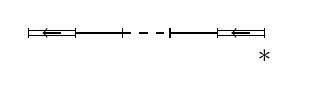
\begin{tikzpicture}[x=.6cm,y=.6cm]
\draw(0,.06)--(1,.06) (0,-.06)--(1,-.06);\draw[->](.7,0)--(.3,0);\draw(1,0)--(2,0);\draw[dashed](2,0)--(3,0);\draw(3,0)--(4,0);\draw(4,.06)--(5,.06) (4,-.06)--(5,-.06);\draw[->](4.7,0)--(4.3,0);\foreach\x in {0,...,5}{\draw(\x,-.1)--(\x,.1);}\node[below]at(5,-.15){$*$};
\end{tikzpicture}\qquad（1）
\end{center}
事实上，容易验证，其余情形 $\Phi_F$ 包含 $G$ 的全部不可倍乘相对根（nonmultipliable relative roots），故断言由 [4，2.23 和 4.3] 得出。在上述例外情形，$\overline G_F^{\mathrm{red}}$ 为特殊正交群，因此不单连通。利用“单连通群中环面的中心化子的导群仍单连通”这一事实，容易得到更一般的结果。称绝对局部 Dynkin 图 $\Delta_1$ 的特殊顶点为好的（good），若它不是该图某个（1）型连通分支的星号顶点。则若 $G$ 半单且单连通，而且 $\bigcup_{v\in I_F}O(v)$ 包含 $\Delta_1$ 每个连通分支中的一个好的特殊顶点，则 $\overline G_F^{\mathrm{red}}$ 的导群单连通。
\origsubsection{3.6}{环面单位群的不动点（Fixed points of groups of units of tori）}
设 $M$ 为 $S$ 的单位群 $S_c=\{s\in S(K)\mid\omega(\chi(s))=0\text{ 对所有 }\chi\in X^*\}$ 的子群。我们要确定：在什么条件下，公寓 $A=A(G,S)$ 恰好等于 $M$ 在 $\mathscr B$ 中的不动点集 $\mathscr B^M$。由 2.2 回顾的建筑性质，$A=\mathscr B^M$，当且仅当对 $A$ 的每个余维一的面 $F$，闭包包含 $F$ 且被 $M$ 固定的室，仅为 $A$ 内具有这些性质的两个室。由 3.5.4，这意味着 $M$ 在 $\overline S(\overline K)$ 中的像 $\overline M$，在 $\overline G_F^{\mathrm{red}}$ 的 $\overline K$ 球面建筑中只有两个不动点。若 $a$ 为 $\Phi_F$ 的两个不可除根之一，这等价于 $a(\overline M)\ne\{1\}$。因此：

\paragraph*{3.6.1.}$A$ 为 $M$ 在 $\mathscr B$ 中完整不动点集的充要条件是，对每个相对根 $a\in\Phi$，有 $a(M)\not\subset1+\mathfrak p$。

特别地，如果 $\overline K$ 至少有四个元素（若 $\overline K\simeq\F_2$），则 $A$ 总是（从不）为 $S_c$ 在 $\mathscr B$ 中的完整不动点集。

前面的讨论还给出如下信息：一个非分裂环面 $S_1$ 在 $K$ 的非分歧 Galois 扩张 $K_1$ 上成为极大分裂环面，则可将 3.6.1 应用于其单位群 $S_{1,c}$ 在 $\mathscr B(G,K_1)$ 上的作用，再利用 2.6.1 作 Galois 下降回到 $\mathscr B$，从而研究 $S_{1,c}$ 的不动点集。例如得到：

若各向异性环面 $S_1$ 在 $K$ 的某个非分歧 Galois 扩张上成为极大分裂环面，则 $S_1(K)$ 在建筑 $\mathscr B$ 中有唯一的不动点。

另一方面，容易证明：若 $S_1$ 是 $G=\SL_2$ 的极大环面，且其分裂域分歧，则 $S_1(K)$ 必固定 $\mathscr B$ 的一个室，也可能固定不止一个室。\footnote{这回答了 G. Lusztig 的一个问题。}对 $\operatorname{PGL}_2$ 中类似的环面 $S_1$，$S_1(K)$ 在 $\mathscr B$ 中可能只有一个不动点，也可能不止一个。
\origsubsection{3.7}{Iwahori 子群；极大紧子群的体积（Iwahori subgroups; volume of maximal compact subgroups）}
本节假设 $G$ 剩余拟分裂；当剩余域 $\overline K$ 有限时，1.10.3保证了这一条件。

为建筑 $\mathscr B$ 的每个室 $C$ 定义一个 $G(K)$ 的子群 $\operatorname{Iw}(C)$，称为对应于 $C$ 的 Iwahori 子群：若 $\overline G_C^\circ$ 为代数群 $\overline G_C$ 的单位分支（见 3.4），则 $\operatorname{Iw}(C)$ 为群 $\overline G_C^\circ(\overline K)$ 在约化同态 $\mathscr G_C(\mathfrak o)\to\overline G_C(\overline K)$ 下于 $\mathscr G_C(\mathfrak o)=G(K)^C$ 中的原像。显然，$G(K)$ 的所有 Iwahori 子群共轭。由 3.5.2，$\overline G_C^\circ$ 可解，故为环面 $\overline T$ 与幺幂群 $\overline U$ 的半直积。由光滑群概形的一般结果，$\operatorname{Iw}(C)$ 是 $\overline T(\overline K)$ 与某个逆极限幂零群（pronilpotent group）$\operatorname{Iw}^u(C)$ 的半直积；若 $\overline K$ 的特征为有限素数 $p$，则 $\operatorname{Iw}^u(C)$ 为pro-$p$ 群（pro-$p$ group）；若 $\overline K$ 有限，$\overline T(\overline K)$ 当然为阶与 $p$ 互素的有限群。

若 $x$ 为 $C$ 的闭包中的一点，则 $\overline G_C^\circ$ 在同态 $\overline\rho_{xC}:\overline G_C\to\overline G_x$ 下的像为 $\overline G_x$ 的一个 Borel 子群 $\overline B$，而 $\overline\rho_{xC}$ 的核是连通幺幂群。因此 $\overline\rho_{xC}$ 将 $\overline G_C^\circ(\overline K)$ 满射到 $\overline B(\overline K)$；再由 3.4.4，$\operatorname{Iw}(C)$ 是 $\overline B(\overline K)$ 在约化同态下于 $G(K)^x=\mathscr G_x(\mathfrak o)$ 中的原像。因此，也可将 $G(K)$ 的 Iwahori 子群定义为：对各 $x\in\mathscr B$，约化群 $\overline G_x$ 的 $\overline K$ Borel 子群在稳定子 $G(K)^x$ 中的原像。

现设 $\overline K$ 有限。则 $G(K)$ 为幺模局部紧群（unimodular locally compact group），Iwahori 子群是紧开子群。因此，存在唯一 Haar 测度 $\mu$，使 Iwahori 子群体积为 $1$。由上，对任意 $x\in\mathscr B$，$G(K)^x$ 关于 $\mu$ 的体积为指数 $[\overline G_x(\overline K):\overline B(\overline K)]$，其中 $\overline B$ 为 $\overline G_x$ 的任一 $\overline K$ Borel 子群。若 $x$ 在包含它的面 $F$ 中处于“一般位置”，则 $\overline G_x=\overline G_F$。已知 $G$ 的局部指标（连同 1.11 的对应 $v\mapsto O(v)$）、$\Delta$ 的顶点集 $I_x$，以及 $\Xi_1=\Xi(G,K_1)$（见 2.5），其中 $K_1$ 为 $K$ 的非分歧闭包，则断言 3.5.2、3.5.3 给出了有效计算这一体积的方法。
\origsubsection{3.8}{超特殊点与子群（Hyperspecial points and subgroups）}
由 3.5.1 与 3.5.3，容易得出 1.10 所定义的 $\mathscr B$ 的超特殊点的如下刻画。

\paragraph*{3.8.1.}$\mathscr B$ 的点 $x$ 超特殊，当且仅当群 $\overline G_x$ 的单位分支约化；此时 $\overline G_x$ 本身连通，因而约化。

还可以证明：$\mathfrak o$ 上一般纤维为 $G$、特殊纤维为约化群的光滑群概形，恰好是超特殊点 $x$ 所对应的概形 $\mathscr G_x$。因此，可将 $G(K)$ 的超特殊子群刻画为这种群概形的单位群。

\paragraph*{3.8.2.}假设 $\overline K$ 有限，且 $G(K)$ 具有超特殊子群（例如，若 $G$ 拟分裂且有非分歧分裂域，此条件成立，见 1.10）；则 $G(K)$ 的超特殊子群，是其全部紧子群中体积最大的那些子群。

利用 3.5 和 3.7，证明并不困难。
\origsubsection{3.9}{整体情形（The global case）}
设 $L$ 为整体域。对 $L$ 的每个有限扩张 $L'$ 及 $L'$ 的每个素位 $v$，以 $\mathfrak o_{L'}$、$\mathfrak o_v$ 分别表示 $L'$ 和其完备化 $L'_v$ 的整数环。设 $H$ 为在 $L$ 上定义的约化线性群。假设将 $H$ 嵌入一般线性群 $\GL_n$，并对上述每组 $L',v$ 定义 $H(\mathfrak o_v)=H(L'_v)\cap\GL_n(\mathfrak o_v)$。也可以通过群概形来描述这个群。考虑由 $L^n$ 中标准格 $\mathfrak o_L^n$ 定义的 $H$ 上的 $\mathfrak o_L$ 群概形结构 $\mathscr H_{\mathfrak o_L}$；更精确地，$\mathscr H_{\mathfrak o_L}$ 是 $H$ 在标准一般线性群概形 $\mathscr{GL}_{n,\mathfrak o_L}$ 中的概形闭包。于是 $H(\mathfrak o_v)=\mathscr H_{\mathfrak o_L}(\mathfrak o_v)$。对包含 $\mathfrak o_L$ 的任一环 $R$，以 $\mathscr H_R$ 表示由 $\mathscr H_{\mathfrak o_L}$ 经基变换所得的 $R$ 上群概形。

\paragraph*{3.9.1.}在 $L$ 的几乎所有有限素位 $v$，$\mathscr H_{\mathfrak o_v}$ 为与建筑 $\mathscr B(H,L_v)$ 的某个超特殊点 $x$ 相联系的群概形 $\mathscr H_x$；因而 $H(\mathfrak o_v)$ 是 $H(L_v)$ 的超特殊子群。

事实上，取 $L$ 的一个使 $H$ 分裂的 Galois 扩张 $L'$，并取一般纤维为 $\mathscr H_{L'}$ 的 $\mathfrak o_{L'}$ 上 Chevalley 群概形 $\mathscr H'_{\mathfrak o_{L'}}$。由于群概形 $\mathscr H_{\mathfrak o_{L'}}$ 与 $\mathscr H'_{\mathfrak o_{L'}}$ 有相同一般纤维，它们在 $L'$ 的几乎所有素位处“相同”。又因 $L'$ 几乎所有素位在其对 $L$ 的限制上非分歧，断言由 3.4.2、3.4.3 及 2.6.1 得到。
\origsubsection{3.10}{例：一般线性群（Example: general linear groups）}
设 $G=\GL_n$。$\GL_n(K)$ 的 Iwahori 子群为与下列子群共轭的子群：\nobreak\footnote{\textbf{译者注（本次校订）：}下式矩阵条件中的最后一个 $i\ge j$ 应为 $i>j$。否则对角元会同时满足 $g_{ii}\in\mathfrak o^\times$ 与 $g_{ii}\in\mathfrak p$，使所定义的集合为空。正确条件为对角元是单位、上三角元属于 $\mathfrak o$、严格下三角元属于 $\mathfrak p$。}
\[
B=\{((g_{ij}))\mid g_{ii}\in\mathfrak o^\times,\ g_{ij}\in\mathfrak o\text{ 若 }i<j,\ g_{ij}\in\mathfrak p\text{ 若 }i\geq j\}.
\]
令 $(b_i)_{1\leq i\leq n}$ 为 $K^n$ 的标准基。对 $1\leq r\leq n$，令 $\Lambda_r$ 为 $K^n$ 中由 $\{b_i/\pi\mid i\leq r\}\cup\{b_i\mid i>r\}$ 生成的格，$P_r$ 为 $\Lambda_r$ 在 $\GL_n(K)$ 中的稳定子。因此，$P_r$ 是全部行列式为单位、且有下列分块形式的矩阵所成的群：
\[
\left(\begin{array}{c|c}
\mathfrak o&\pi^{-1}\mathfrak o\\\hline
\pi\mathfrak o&\mathfrak o
\end{array}\right),\qquad\text{分块大小为 }r\text{ 与 }n-r.
\]
此记号表示，左上角为系数在 $\mathfrak o$ 中的 $r\times r$ 矩阵，右上角为系数在 $\pi^{-1}\mathfrak o$ 中的 $r\times(n-r)$ 矩阵，等等。群 $B$ 是 1.14 所述室 $C$ 在 $\GL_n(K)$ 中的中心化子。子群 $P_r$ 均特殊，每个特殊子群都与其中任一个共轭。各 $P_r$ 是 $\overline C$ 中各一维面上点的稳定子；沿用 2.9 的记号，$P_r$ 固定的点对应于下述形式的范数：
\[
(x_1,\ldots,x_n)\longmapsto\inf\bigl(
\{\omega(x_i)+\omega(\pi)-c\mid i\leq r\}\cup\{\omega(x_i)-c\mid i>r\}\bigr),
\]
其中 $c\in\R$。若 $v$ 为这种点，则概形 $\mathscr G_v$ 是格 $\Lambda_r$ 所定义的“$\GL_n$ 上”的 Chevalley 概形。要描述单位群为 $B$ 的概形 $\mathscr G_C$，可用 $n$ 个标准表示之和将 $\GL_n$ 嵌入 $\GL_{n^2}$，并考虑 $K^{n^2}$ 中的格 $\Lambda_1\oplus\cdots\oplus\Lambda_n$。

注意，$B$ 是 $C$ 中任一点的稳定子。对 $G=\operatorname{PGL}_n$，相应陈述不成立。例如，由 $B$ 与线性变换
\[
b_1\longmapsto b_2\longmapsto\cdots\longmapsto b_n\longmapsto b_1\pi^{-1}\tag{3.10(1)}
\]
生成的群在 $\operatorname{PGL}_n(K)$ 中的像，是投影 $C$ 所得的 $\mathscr B(\operatorname{PGL}_n,K)$ 的室的“重心”$y$ 的稳定子。它也是 $\operatorname{PGL}_n(K)$ 的极大有界子群。概形 $\mathscr G_y$ 可用 $G=\operatorname{PGL}_n$ 的 Lie 代数中的一个格描述，$G$ 通过伴随表示在此 Lie 代数上作用。若 $F$ 为由（1）在 $\operatorname{PGL}_n$ 中的像模 $\mathfrak p$ 约化所生成的 $n$ 阶循环群，则 $\overline G_y$ 是 $F$ 与某个连通群的半直积；特别地，其分支群为 $n$ 阶循环群。
\origsubsection{3.11}{例：奇数维拟分裂特殊酉群（Example: quasi-split special unitary group in odd dimension）}
沿用 1.15 的全部假设与记号，以 $\mathfrak o_L$ 表示 $L$ 的整数环。取 $\lambda\in L$，满足 $\lambda+\lambda^\tau+1=0$、$\omega(\lambda)=\delta$（回顾 $\delta=\sup\{\omega(d)\mid d\in L,d+d^\tau+1=0\}$）。假设一致化元 $\pi_1$ 选得满足 $(\lambda\pi_1)+(\lambda\pi_1)^\tau=0$；$L/K$ 非分歧时这种选择显然可作，分歧时由 1.15（6）得出。

令 $(b_i)_{-n\leq i\leq n}$ 为 $L^{2n+1}$ 的标准基。对 $0\leq r\leq n$，考虑基 $(b_i^{(r)})$：当 $i<-r$ 时 $b_i^{(r)}=b_i/\pi_1$；当 $-r\leq i\leq0$ 时 $b_i^{(r)}=b_i$；当 $i>0$ 时 $b_i^{(r)}=\lambda b_i$。记此基生成的 $\mathfrak o_L$ 格为 $\Lambda_r$。若 $\delta=\omega(\lambda)=0$（除 $L/K$ 分歧且 $\operatorname{char}\overline K=2$ 外总如此），$\Lambda_r$ 也由基 $\{b_i/\pi_1\mid i<-r\}\cup\{b_i\mid i\geq-r\}$ 生成。$\Lambda_r$ 在 $G(K)$ 中的稳定子 $P_r$，也是由下式确定的点 $v_r\in V=A\subset\mathscr B$（按 1.15 的约定）的稳定子：
\[
a_i(v_r)=\begin{cases}\frac12\delta,&i\leq r,\\\frac12(\delta+\omega(\pi_1)),&i>r.\end{cases}
\]
各点 $v_r$ 是由不等式 $\frac12\delta<a_1<\cdots<a_n<\frac12\delta+\frac12\omega(\pi_1)$ 定义的室的顶点。通过 $v\mapsto I_v$，它们按自然的从左到右顺序，对应于 1.15 的图（9）与（10）的顶点。概形 $\mathscr G_{v_r}$ 是由格 $\Lambda_r$ 定义的 $G$ 上的 $\mathfrak o_L$ 结构。

现在简要研究将 $\mathscr G_{v_r}$ 模 $\mathfrak p$ 约化所得的代数群 $\overline G_{v_r}$。固定 $r$，以带撇字母表示关于基 $(b_i^{(r)})$ 的坐标。在这些坐标中，Hermite 型 $h$ 为
\[
\begin{aligned}
h((x'_i),(y'_i))={}&x_0'{}^\tau y'_0+
\sum_{i=1}^r(\lambda^\tau x_i'{}^\tau y'_{-i}+\lambda x_{-i}'{}^\tau y'_i)\\
&+\frac{\lambda^\tau}{\pi_1}\sum_{i=r+1}^n(x_i'{}^\tau y'_{-i}-x_{-i}'{}^\tau y'_i).
\end{aligned}
\]
令 $\widetilde E=\Lambda_r/\pi\Lambda_r$。它是 $\overline K$ 上的 $2(2n+1)$ 维向量空间。可证明自然态射 $\overline G_{v_r}\to\GL(\widetilde E)$ 为单态射（monomorphism）；换言之，$\overline G_{v_r}$ 可视为 $\GL(\widetilde E)$ 的子群。下面分别讨论非分歧与分歧情形。

\paragraph*{第一种情形：L/K 非分歧}此时 $\widetilde E$ 也是 $L$ 的剩余域 $\overline L$ 上的向量空间。反 Hermite 型（antihermitian form）$\pi_1h/\lambda^\tau$ 模 $\pi_1$ 约化为 $\widetilde E$ 上的反 Hermite 型
\[
\overline h_1:((\widetilde x'_i),(\widetilde y'_i))\longmapsto
\sum_{i=r+1}^n(\widetilde x_i'{}^\tau\widetilde y'_{-i}-\widetilde x_{-i}'{}^\tau\widetilde y'_i),
\]
其中横线或波浪号表示相应的约化。令 $\widetilde E_0$ 为此型的核，由 $|i|>r$ 时 $\widetilde x'_i=0$ 定义；令 $\Lambda_{r,0}$ 为 $\widetilde E_0$ 在 $\Lambda_r$ 中的原像。考察 $h$ 在 $\Lambda_{r,0}\times\Lambda_{r,0}$ 上的限制，模 $\mathfrak p$ 约化后成为 $\widetilde E_0$ 上的 Hermite 型
\[
\overline h_2:((\widetilde x'_i)_{-r\leq i\leq r},(\widetilde y'_i)_{-r\leq i\leq r})\longmapsto
\widetilde x_0'{}^\tau\widetilde y'_0+
\sum_{i=1}^r(\overline\lambda^\tau\widetilde x_i'{}^\tau\widetilde y'_{-i}
+\overline\lambda\widetilde x_{-i}'{}^\tau\widetilde y'_i).
\]
最后，$\overline G_{v_r}$ 可描述为型对 $(\overline h_1,\overline h_2)$ 在群 $R_{\overline L/\overline K}(\SL_{\overline L}(\widetilde E))$ 中的稳定子；此群即将 $\overline L$ 向量空间 $\widetilde E$ 的特殊线性群通过标量限制“看作 $\overline K$ 上的代数群”。令 $\widetilde E_1$ 为 $\widetilde E$ 中由 $-r\leq i\leq r$ 时 $\widetilde x'_i=0$ 定义的子空间，以 $\widetilde h_1$ 表示 $\overline h_1$ 在 $\widetilde E_1\times\widetilde E_1$ 上的限制。则 $\overline G_{v_r}$ 显然包含群 $\operatorname{SU}(\widetilde h_1)\times\operatorname{SU}(\overline h_2)$，它正是其 Levi 子群 $\overline G_{v_r}^{\mathrm{red}}$（见 3.5）。\footnote{\textbf{译者注（本次校订）：}当两个非退化块均非零时，这里列出的 $\operatorname{SU}(\widetilde h_1)\times\operatorname{SU}(\overline h_2)$ 是 Levi 子群的导出群；完整的 Levi 子群为 $\operatorname{S}(\operatorname U(\widetilde h_1)\times\operatorname U(\overline h_2))$，即两块酉变换的行列式乘积为一的群。两块的行列式不必分别为一，因此还有一个一维中心环面。}注意，符合 3.5.1，从 1.15 的图（9）删去第 $(r+1)$ 个顶点及邻接边所得图为 $BC_r\times C_{n-r}$ 型，这确实为 $\operatorname{SU}(\widetilde h_1)\times\operatorname{SU}(\overline h_2)$ 的相对根系类型。

\paragraph*{第二种情形：L/K 分歧}此时，$\Lambda_r$ 中的标量乘法 $\pi_1$，模 $\pi$ 约化后给出自同态 $\nu:\widetilde E\to\widetilde E$，它显然被 $\overline G_{v_r}$ 中心化，且核等于像 $\nu(\widetilde E)$。商 $\overline E=\widetilde E/\nu(\widetilde E)$ 典范同构于 $\Lambda_r/\pi_1\Lambda_r$，将二者等同。$\nu$ 被 $\overline G_{v_r}$ 中心化，故投影 $\widetilde E\to\overline E$ 诱导 $\overline K$ 代数群同态 $\overline G_{v_r}\to\GL(\overline E)$，其核幺幂。这里只描述此同态的像，记作 $\overline G'_{v_r}$；确定 $\overline G_{v_r}$ 的完整结构留作练习。

将反 Hermite 型 $\pi_1h/\lambda^\tau$ 模 $\pi_1$ 约化，得到 $\overline E$ 上的交错型（alternating form）
\[
\overline h_1:((\overline x'_i),(\overline y'_i))\longmapsto
\sum_{i=r+1}^n(\overline x'_i\overline y'_{-i}-\overline x'_{-i}\overline y'_i).
\]
令 $\overline E_0$ 为此型的核，由 $|i|>r$ 时 $\overline x'_i=0$ 定义；$\Lambda_{r,0}$ 为其在 $\Lambda_r$ 中的原像。现考察 $q:\Lambda_{r,0}\to K$，$q(x)=h(x,x)$。经约化后，它成为二次型 $\overline q:\overline E_0\to\overline K$：
\[
\overline q((\overline x'_i)_{-r\leq i\leq r})=\overline x_0'{}^2-
\sum_{i=1}^r\overline x'_{-i}\overline x'_i.
\]
最后，$\overline G'_{v_r}$ 是 $\SL(\overline E)$ 中保持 $\overline h_1$、且在 $\overline E_0$ 上诱导（既约）群 $\operatorname{SO}(\overline q)$ 的一个元素的全部元素组成的群。令 $\overline E_1$ 为由 $-r<i<r$ 时 $\overline x'_i=0$ 定义的 $\overline E$ 的子空间，以 $\widetilde h_1$ 表示 $\overline h_1$ 在 $\overline E_1\times\overline E_1$ 上的限制。\footnote{\textbf{译者注（本次校订）：}此处定义 $\overline E_1$ 时，坐标范围应为 $-r\le i\le r$，即应令这些坐标全部为零。使用严格不等式会留下核中的端点坐标（$r=0$ 时也会留下零坐标），使 $\widetilde h_1$ 退化，不能得到所写的辛群。}则 $\operatorname{Sp}(\widetilde h_1)\times\operatorname{SO}(\overline q)$ 是 $\overline G'_{v_r}$ 的 Levi 子群，它是 $\overline G_{v_r}$ 的 Levi 子群 $\overline G_{v_r}^{\mathrm{red}}$ 在该群中的同构像。如非分歧情形一样，可检验 3.5.1；此时使用 1.15 的图（10），得到 $\overline G_{v_r}^{\mathrm{red}}$ 的根系类型 $B_r\times C_{n-r}$。

注意，即使在非分歧情形，也可不用 $h$ 在 $\Lambda_{r,0}\times\Lambda_{r,0}$ 上的限制，而考察其“收缩”$q:\Lambda_{r,0}\to K$、$q(x)=h(x,x)$，这样，两种情形便可采用更统一的处理方式。另一方面，引入 $\lambda$ 是为尽量减少情形划分；在非分歧情形，以及 $\operatorname{char}\overline K\ne2$ 时，可以到处以 $1$ 代替 $\lambda$，使方程有所简化。
\origsubsection{3.12}{例：拟分裂但不分裂的特殊正交群（Example: quasi-split but nonsplit special orthogonal group）}
现采用 1.16 的假设与记号，只是取 $G$ 为特殊正交群 $\operatorname{SO}(q)$。这里只讨论这一例子的一个方面：构造建筑的一个顶点 $v$，使 $\overline G_v$ 不连通。假设 $L/K$ 非分歧。令 $\Lambda$ 为 $K^n\oplus L\oplus K^n$ 中的格 $\mathfrak o^n\oplus\pi\mathfrak o_L\oplus\mathfrak o^n$，其中 $\mathfrak o_L$ 为 $L$ 的整数环。$\Lambda$ 在 $G(K)$ 中的稳定子 $P$，也是由 $a_i(v)=\frac12\omega(\pi)$（$1\leq i\leq n$）定义的点 $v\in V\subset A$ 的稳定子；它是 1.16 所描述的室的一个顶点。在 1.16 的图（1）中，$I_v$ 为最左端的顶点。如 3.11，可将 $\overline G_v$ 描述为 $\GL(\widetilde E)$ 的子群，其中 $\widetilde E=\Lambda/\pi\Lambda$ 为 $\overline K$ 向量空间。型 $q$ 在 $\Lambda$ 上的限制经约化，成为 $\widetilde E$ 上的二次型 $\widetilde q:(\widetilde x_i)_{-n\leq i\leq n}\mapsto\sum_{i=1}^n\widetilde x_{-i}\widetilde x_i$，其中横线或波浪号表示相应的约化（$i=0$ 时 $\widetilde x_i$ 属于 $L$ 的剩余域，否则属于 $\overline K$）。令 $\widetilde E_0$ 为 $\widetilde q$ 的二维核，由 $i\ne0$ 时 $\widetilde x_i=0$ 定义；令 $\overline q$ 为 $\widetilde q$ 在 $\overline E=\widetilde E/\widetilde E_0$ 上诱导的二次型。显然，$\overline G_v$ 保持型 $\widetilde q$。因此投影 $\widetilde E\to\overline E$ 诱导 $\overline K$ 同态 $\overline G_v\to O(\overline q)$。可验证，此同态满射（特别地，$\overline G_v$ 不连通），并将 $\overline G_v^{\mathrm{red}}$ 同构地映到 $\operatorname{SO}(\overline q)$。\footnote{\textbf{译者注（本次校订）：}这个映射在 Levi 子群上还有一个各向异性的一维环面核。原二次型的 $L$ 分量上的范数一变换保留格 $\Lambda$，经约化后仍在二维核 $\widetilde E_0$ 上非平凡作用，却在 $\overline E$ 上作用平凡。因此完整的连通 Levi 子群为 $\operatorname{SO}(\overline q)\times\operatorname{SO}(N_{\overline L/\overline K})$；到第一因子的投影不能称为同构。}若 $\tau$ 为 $L$ 的非平凡 $K$ 自同构，则属于 $P$ 的线性变换
\[
(x_i)_{-n\leq i\leq n}\longmapsto(x_n,x_{-n+1},\ldots,x_{-1},x_0^\tau,x_1,\ldots,x_{n-1},x_{-n})
\]
经约化给出 $\overline G_v(\overline K)$ 的一个元素，它映入 $O(\overline q)$，但不映入 $\operatorname{SO}(\overline q)$。

\origsection{4}{分类（Classification）}
\origsubsection{4.1}{引言（Introduction）}
最后讨论剩余域 $\overline K$ 有限时单群的分类；从现在起均作这一假设。回顾，在特征零情形，此分类最早由 M. Kneser [16] 给出。表 4.2、4.3 连同 4.5 的说明，列出 $K$ 上绝对拟单群（absolutely quasi-simple groups）的所有中心同源类（central isogeny classes）。每一类群都列出以下信息；其中 $K_1$ 表示 $K$ 的非分歧闭包。

形如 ${}^aX$ 的名称：符号 $X$ 表示绝对局部 Dynkin 图 $\Delta_1$（1.11），记号同 [8，1.4.6]，但本文 $C$-$BC$ 对应于 [8] 的 $C$-$BC^{\mathrm{III}}$；$a$ 为 $\Gal(K_1/K)$ 在 $\Delta_1$ 上诱导的自同构群的阶。剩余分裂群的 $a=1$，记号中省去上标 $a$。注意，$X$ 右侧的下标为在 $K_1$ 上的相对秩，因而等于 $\Delta_1$ 的顶点数减一。若不同类型原本会得到同一名称，就用撇号、双撇号等加以区分。

按 [8] 的记号表示仿射根系（或 échelonnage）的符号：剩余分裂情形中，此符号与类型名称相同，故不单列。符号的右侧部分给出相对根系 $\Phi$ 的类型；特别地，右下标为在 $K$ 上的相对秩，因而等于相对局部 Dynkin 图 $\Delta$ 的顶点数减一。

局部指标（1.11）、相对局部 Dynkin 图 $\Delta$（1.8）及各顶点所带的整数 $d(v)$（1.8）：$\Gal(K_1/K)$ 通过 $a$ 阶循环群在 $\Delta_1$ 上的作用，基本由其在 $\Delta_1$ 顶点集中的轨道刻画。图中如下展示轨道：对应于 $\Delta$ 顶点 $v$ 的轨道 $O(v)$（1.11）的元素，紧靠排列在与 $v$ 相同的竖线上（$\Delta$ 的两个顶点位于同一竖线的少数情形，例如 ${}^2D_n$、${}^2D''_{2m}$ 等，$v\mapsto O(v)$ 的对应由图的画法应当清楚）。由于 $\overline K$ 有限，$G$ 剩余拟分裂（1.10.3），因此除了唯一的各向异性类型 ${}^dA_{d-1}$ 外，$\Delta_1$ 全部顶点都是标识顶点（1.11），无须像 [22] 那样另外圈出轨道。超特殊顶点（1.10）标以 hs，其他特殊顶点（1.9）标以 s。

按 [3]、[22] 中通常定义的型指标：为简便起见，不画出这一指标，而用 [22] 记号中的相应符号表示。回顾，这一符号除其他信息外，还含有群的绝对类型、绝对秩、相对秩（表示 $\Phi_{\mathrm{af}}$ 的符号已给出），以及 $K$ 的可分闭包的 Galois 群在通常 Dynkin 图上诱导的自同构群的阶。

$A_n$ 的内形式（inner forms）较适合用文字描述，因此相应条目以文字代替图。
\origsubsection{4.2}{剩余分裂群（Residually split groups）}
\begin{longtable}{p{.20\linewidth}p{.52\linewidth}p{.19\linewidth}}
\toprule 名称 & 局部 Dynkin 图 & 指标 [22] \\\midrule\endhead
$A_n\ (n\geq2)$ & 长度为 $n+1$ 的环，全部顶点均超特殊 & ${}^1A_{n,n}^{(1)}$\\[8pt]
$A_1$ & \begin{tikzpicture}[x=.43cm,y=.43cm,line width=.5pt]
\coordinate (n0) at (0,0);\draw(0,{0-.08})--(0,{0+.08});
\coordinate (n1) at (1,0);\draw(1,{0-.08})--(1,{0+.08});
\draw[line width=2pt](n0)--(n1);
\node[below]at($(n0)+(0,-.12)$){hs};
\node[below]at($(n1)+(0,-.12)$){hs};
\end{tikzpicture} & ${}^1A_{1,1}^{(1)}$\\[10pt]
$B_n\ (n\geq3)$ & \begin{tikzpicture}[x=.43cm,y=.43cm,line width=.5pt]
\coordinate (n0) at (0,0);\draw(0,{0-.08})--(0,{0+.08});
\coordinate (n1) at (1,0);\draw(1,{0-.08})--(1,{0+.08});
\coordinate (n2) at (2,0);\draw(2,{0-.08})--(2,{0+.08});
\coordinate (n3) at (3,0);\draw(3,{0-.08})--(3,{0+.08});
\coordinate (n4) at (4,0);\draw(4,{0-.08})--(4,{0+.08});
\coordinate (n5) at (5,0.8);\draw(5,{0.8-.08})--(5,{0.8+.08});
\coordinate (n6) at (5,-0.8);\draw(5,{-0.8-.08})--(5,{-0.8+.08});
\draw($(n0)+(0,-0.06)$)--($(n1)+(0,-0.06)$);
\draw($(n0)+(0,0.06)$)--($(n1)+(0,0.06)$);
\draw[->]($(n1)!.3!(n0)$)--($(n1)!.7!(n0)$);
\draw[solid](n1)--(n2);
\draw[dashed](n2)--(n3);
\draw[solid](n3)--(n4);
\draw[solid](n4)--(n5);
\draw[solid](n4)--(n6);
\node[below]at($(n5)+(0,-.12)$){hs};
\node[below]at($(n6)+(0,-.12)$){hs};
\end{tikzpicture} & $B_{n,n}$\\[10pt]
$B\text{-}C_n\ (n\geq3)$ & \begin{tikzpicture}[x=.43cm,y=.43cm,line width=.5pt]
\coordinate (n0) at (0,0);\draw(0,{0-.08})--(0,{0+.08});
\coordinate (n1) at (1,0);\draw(1,{0-.08})--(1,{0+.08});
\coordinate (n2) at (2,0);\draw(2,{0-.08})--(2,{0+.08});
\coordinate (n3) at (3,0);\draw(3,{0-.08})--(3,{0+.08});
\coordinate (n4) at (4,0);\draw(4,{0-.08})--(4,{0+.08});
\coordinate (n5) at (5,0.8);\draw(5,{0.8-.08})--(5,{0.8+.08});
\coordinate (n6) at (5,-0.8);\draw(5,{-0.8-.08})--(5,{-0.8+.08});
\draw($(n0)+(0,-0.06)$)--($(n1)+(0,-0.06)$);
\draw($(n0)+(0,0.06)$)--($(n1)+(0,0.06)$);
\draw[->]($(n0)!.3!(n1)$)--($(n0)!.7!(n1)$);
\draw[solid](n1)--(n2);
\draw[dashed](n2)--(n3);
\draw[solid](n3)--(n4);
\draw[solid](n4)--(n5);
\draw[solid](n4)--(n6);
\node[below]at($(n5)+(0,-.12)$){s};
\node[below]at($(n6)+(0,-.12)$){s};
\end{tikzpicture} & ${}^2A_{2n-1,n}^{(1)}$\\[10pt]
$C_n\ (n\geq2)$ & \begin{tikzpicture}[x=.43cm,y=.43cm,line width=.5pt]
\coordinate (n0) at (0,0);\draw(0,{0-.08})--(0,{0+.08});
\coordinate (n1) at (1,0);\draw(1,{0-.08})--(1,{0+.08});
\coordinate (n2) at (2,0);\draw(2,{0-.08})--(2,{0+.08});
\coordinate (n3) at (3,0);\draw(3,{0-.08})--(3,{0+.08});
\coordinate (n4) at (4,0);\draw(4,{0-.08})--(4,{0+.08});
\coordinate (n5) at (5,0);\draw(5,{0-.08})--(5,{0+.08});
\draw($(n0)+(0,-0.06)$)--($(n1)+(0,-0.06)$);
\draw($(n0)+(0,0.06)$)--($(n1)+(0,0.06)$);
\draw[->]($(n0)!.3!(n1)$)--($(n0)!.7!(n1)$);
\draw[solid](n1)--(n2);
\draw[dashed](n2)--(n3);
\draw[solid](n3)--(n4);
\draw($(n4)+(0,-0.06)$)--($(n5)+(0,-0.06)$);
\draw($(n4)+(0,0.06)$)--($(n5)+(0,0.06)$);
\draw[->]($(n5)!.3!(n4)$)--($(n5)!.7!(n4)$);
\node[below]at($(n0)+(0,-.12)$){hs};
\node[below]at($(n5)+(0,-.12)$){hs};
\end{tikzpicture} & $C_{n,n}^{(1)}$\\[10pt]
$C\text{-}B_n\ (n\geq2)$ & \begin{tikzpicture}[x=.43cm,y=.43cm,line width=.5pt]
\coordinate (n0) at (0,0);\draw(0,{0-.08})--(0,{0+.08});
\coordinate (n1) at (1,0);\draw(1,{0-.08})--(1,{0+.08});
\coordinate (n2) at (2,0);\draw(2,{0-.08})--(2,{0+.08});
\coordinate (n3) at (3,0);\draw(3,{0-.08})--(3,{0+.08});
\coordinate (n4) at (4,0);\draw(4,{0-.08})--(4,{0+.08});
\coordinate (n5) at (5,0);\draw(5,{0-.08})--(5,{0+.08});
\draw($(n0)+(0,-0.06)$)--($(n1)+(0,-0.06)$);
\draw($(n0)+(0,0.06)$)--($(n1)+(0,0.06)$);
\draw[->]($(n1)!.3!(n0)$)--($(n1)!.7!(n0)$);
\draw[solid](n1)--(n2);
\draw[dashed](n2)--(n3);
\draw[solid](n3)--(n4);
\draw($(n4)+(0,-0.06)$)--($(n5)+(0,-0.06)$);
\draw($(n4)+(0,0.06)$)--($(n5)+(0,0.06)$);
\draw[->]($(n4)!.3!(n5)$)--($(n4)!.7!(n5)$);
\node[below]at($(n0)+(0,-.12)$){s};
\node[below]at($(n5)+(0,-.12)$){s};
\end{tikzpicture} & ${}^2D_{n+1,n}^{(1)}$\\[10pt]
$C\text{-}BC_n\ (n\geq2)$ & \begin{tikzpicture}[x=.43cm,y=.43cm,line width=.5pt]
\coordinate (n0) at (0,0);\draw(0,{0-.08})--(0,{0+.08});
\coordinate (n1) at (1,0);\draw(1,{0-.08})--(1,{0+.08});
\coordinate (n2) at (2,0);\draw(2,{0-.08})--(2,{0+.08});
\coordinate (n3) at (3,0);\draw(3,{0-.08})--(3,{0+.08});
\coordinate (n4) at (4,0);\draw(4,{0-.08})--(4,{0+.08});
\coordinate (n5) at (5,0);\draw(5,{0-.08})--(5,{0+.08});
\draw($(n0)+(0,-0.06)$)--($(n1)+(0,-0.06)$);
\draw($(n0)+(0,0.06)$)--($(n1)+(0,0.06)$);
\draw[->]($(n1)!.3!(n0)$)--($(n1)!.7!(n0)$);
\draw[solid](n1)--(n2);
\draw[dashed](n2)--(n3);
\draw[solid](n3)--(n4);
\draw($(n4)+(0,-0.06)$)--($(n5)+(0,-0.06)$);
\draw($(n4)+(0,0.06)$)--($(n5)+(0,0.06)$);
\draw[->]($(n5)!.3!(n4)$)--($(n5)!.7!(n4)$);
\node[below]at($(n0)+(0,-.12)$){s};
\node[below]at($(n5)+(0,-.12)$){s};
\end{tikzpicture} & ${}^2A_{2n,n}^{(1)}$\\[10pt]
$C\text{-}BC_1$ & \begin{tikzpicture}[x=.43cm,y=.43cm,line width=.5pt]
\coordinate (n0) at (0,0);\draw(0,{0-.08})--(0,{0+.08});
\coordinate (n1) at (1,0);\draw(1,{0-.08})--(1,{0+.08});
\draw[line width=2pt](n0)--(n1);
\draw[->]($(n1)!.3!(n0)$)--($(n1)!.7!(n0)$);
\node[below]at($(n0)+(0,-.12)$){s};
\node[below]at($(n1)+(0,-.12)$){s};
\end{tikzpicture} & ${}^2A_{2,1}^{(1)}$\\[10pt]
$D_n\ (n\geq4)$ & \begin{tikzpicture}[x=.43cm,y=.43cm,line width=.5pt]
\coordinate (n0) at (-1,0.8);\draw(-1,{0.8-.08})--(-1,{0.8+.08});
\coordinate (n1) at (-1,-0.8);\draw(-1,{-0.8-.08})--(-1,{-0.8+.08});
\coordinate (n2) at (0,0);\draw(0,{0-.08})--(0,{0+.08});
\coordinate (n3) at (1,0);\draw(1,{0-.08})--(1,{0+.08});
\coordinate (n4) at (2,0);\draw(2,{0-.08})--(2,{0+.08});
\coordinate (n5) at (3,0);\draw(3,{0-.08})--(3,{0+.08});
\coordinate (n6) at (4,0.8);\draw(4,{0.8-.08})--(4,{0.8+.08});
\coordinate (n7) at (4,-0.8);\draw(4,{-0.8-.08})--(4,{-0.8+.08});
\draw[solid](n0)--(n2);
\draw[solid](n1)--(n2);
\draw[solid](n2)--(n3);
\draw[dashed](n3)--(n4);
\draw[solid](n4)--(n5);
\draw[solid](n5)--(n6);
\draw[solid](n5)--(n7);
\node[below]at($(n0)+(0,-.12)$){hs};
\node[below]at($(n1)+(0,-.12)$){hs};
\node[below]at($(n6)+(0,-.12)$){hs};
\node[below]at($(n7)+(0,-.12)$){hs};
\end{tikzpicture} & ${}^1D_{n,n}^{(1)}$\\[10pt]
$E_6$ & \begin{tikzpicture}[x=.43cm,y=.43cm,line width=.5pt]
\coordinate (n0) at (0,0);\draw(0,{0-.08})--(0,{0+.08});
\coordinate (n1) at (1,0);\draw(1,{0-.08})--(1,{0+.08});
\coordinate (n2) at (2,0);\draw(2,{0-.08})--(2,{0+.08});
\coordinate (n3) at (3,1);\draw(3,{1-.08})--(3,{1+.08});
\coordinate (n4) at (4,2);\draw(4,{2-.08})--(4,{2+.08});
\coordinate (n5) at (3,-1);\draw(3,{-1-.08})--(3,{-1+.08});
\coordinate (n6) at (4,-2);\draw(4,{-2-.08})--(4,{-2+.08});
\draw[solid](n0)--(n1);
\draw[solid](n1)--(n2);
\draw[solid](n2)--(n3);
\draw[solid](n3)--(n4);
\draw[solid](n2)--(n5);
\draw[solid](n5)--(n6);
\node[below]at($(n0)+(0,-.12)$){hs};
\node[below]at($(n4)+(0,-.12)$){hs};
\node[below]at($(n6)+(0,-.12)$){hs};
\end{tikzpicture} & ${}^1E_{6,6}^0$\\[10pt]
$E_7$ & \begin{tikzpicture}[x=.43cm,y=.43cm,line width=.5pt]
\coordinate (n0) at (0,0);\draw(0,{0-.08})--(0,{0+.08});
\coordinate (n1) at (1,0);\draw(1,{0-.08})--(1,{0+.08});
\coordinate (n2) at (2,0);\draw(2,{0-.08})--(2,{0+.08});
\coordinate (n3) at (3,0);\draw(3,{0-.08})--(3,{0+.08});
\coordinate (n4) at (4,0);\draw(4,{0-.08})--(4,{0+.08});
\coordinate (n5) at (5,0);\draw(5,{0-.08})--(5,{0+.08});
\coordinate (n6) at (6,0);\draw(6,{0-.08})--(6,{0+.08});
\coordinate (n7) at (3,1);\draw(3,{1-.08})--(3,{1+.08});
\draw[solid](n0)--(n1);
\draw[solid](n1)--(n2);
\draw[solid](n2)--(n3);
\draw[solid](n3)--(n4);
\draw[solid](n4)--(n5);
\draw[solid](n5)--(n6);
\draw[solid](n3)--(n7);
\node[below]at($(n0)+(0,-.12)$){hs};
\node[below]at($(n6)+(0,-.12)$){hs};
\end{tikzpicture} & $E_{7,7}^0$\\[10pt]
$E_8$ & \begin{tikzpicture}[x=.43cm,y=.43cm,line width=.5pt]
\coordinate (n0) at (0,0);\draw(0,{0-.08})--(0,{0+.08});
\coordinate (n1) at (1,0);\draw(1,{0-.08})--(1,{0+.08});
\coordinate (n2) at (2,0);\draw(2,{0-.08})--(2,{0+.08});
\coordinate (n3) at (3,0);\draw(3,{0-.08})--(3,{0+.08});
\coordinate (n4) at (4,0);\draw(4,{0-.08})--(4,{0+.08});
\coordinate (n5) at (5,0);\draw(5,{0-.08})--(5,{0+.08});
\coordinate (n6) at (6,0);\draw(6,{0-.08})--(6,{0+.08});
\coordinate (n7) at (7,0);\draw(7,{0-.08})--(7,{0+.08});
\coordinate (n8) at (5,1);\draw(5,{1-.08})--(5,{1+.08});
\draw[solid](n0)--(n1);
\draw[solid](n1)--(n2);
\draw[solid](n2)--(n3);
\draw[solid](n3)--(n4);
\draw[solid](n4)--(n5);
\draw[solid](n5)--(n6);
\draw[solid](n6)--(n7);
\draw[solid](n5)--(n8);
\node[below]at($(n0)+(0,-.12)$){hs};
\end{tikzpicture} & $E_{8,8}^0$\\[10pt]
$F_4$ & \begin{tikzpicture}[x=.43cm,y=.43cm,line width=.5pt]
\coordinate (n0) at (0,0);\draw(0,{0-.08})--(0,{0+.08});
\coordinate (n1) at (1,0);\draw(1,{0-.08})--(1,{0+.08});
\coordinate (n2) at (2,0);\draw(2,{0-.08})--(2,{0+.08});
\coordinate (n3) at (3,0);\draw(3,{0-.08})--(3,{0+.08});
\coordinate (n4) at (4,0);\draw(4,{0-.08})--(4,{0+.08});
\draw[solid](n0)--(n1);
\draw[solid](n1)--(n2);
\draw($(n2)+(0,-0.06)$)--($(n3)+(0,-0.06)$);
\draw($(n2)+(0,0.06)$)--($(n3)+(0,0.06)$);
\draw[->]($(n2)!.3!(n3)$)--($(n2)!.7!(n3)$);
\draw[solid](n3)--(n4);
\node[below]at($(n0)+(0,-.12)$){hs};
\end{tikzpicture} & $F_{4,4}^0$\\[10pt]
$F_4^{\mathrm I}$ & \begin{tikzpicture}[x=.43cm,y=.43cm,line width=.5pt]
\coordinate (n0) at (0,0);\draw(0,{0-.08})--(0,{0+.08});
\coordinate (n1) at (1,0);\draw(1,{0-.08})--(1,{0+.08});
\coordinate (n2) at (2,0);\draw(2,{0-.08})--(2,{0+.08});
\coordinate (n3) at (3,0);\draw(3,{0-.08})--(3,{0+.08});
\coordinate (n4) at (4,0);\draw(4,{0-.08})--(4,{0+.08});
\draw[solid](n0)--(n1);
\draw[solid](n1)--(n2);
\draw($(n2)+(0,-0.06)$)--($(n3)+(0,-0.06)$);
\draw($(n2)+(0,0.06)$)--($(n3)+(0,0.06)$);
\draw[->]($(n3)!.3!(n2)$)--($(n3)!.7!(n2)$);
\draw[solid](n3)--(n4);
\node[below]at($(n0)+(0,-.12)$){s};
\end{tikzpicture} & ${}^2E_{6,4}^2$\\[10pt]
$G_2$ & \begin{tikzpicture}[x=.43cm,y=.43cm,line width=.5pt]
\coordinate (n0) at (0,0);\draw(0,{0-.08})--(0,{0+.08});
\coordinate (n1) at (1,0);\draw(1,{0-.08})--(1,{0+.08});
\coordinate (n2) at (2,0);\draw(2,{0-.08})--(2,{0+.08});
\draw[solid](n0)--(n1);
\draw($(n1)+(0,-0.08)$)--($(n2)+(0,-0.08)$);
\draw($(n1)+(0,0)$)--($(n2)+(0,0)$);
\draw($(n1)+(0,0.08)$)--($(n2)+(0,0.08)$);
\draw[->]($(n1)!.3!(n2)$)--($(n1)!.7!(n2)$);
\node[below]at($(n0)+(0,-.12)$){hs};
\end{tikzpicture} & $G_{2,2}$\\[10pt]
$G_2^{\mathrm I}$ & \begin{tikzpicture}[x=.43cm,y=.43cm,line width=.5pt]
\coordinate (n0) at (0,0);\draw(0,{0-.08})--(0,{0+.08});
\coordinate (n1) at (1,0);\draw(1,{0-.08})--(1,{0+.08});
\coordinate (n2) at (2,0);\draw(2,{0-.08})--(2,{0+.08});
\draw[solid](n0)--(n1);
\draw($(n1)+(0,-0.08)$)--($(n2)+(0,-0.08)$);
\draw($(n1)+(0,0)$)--($(n2)+(0,0)$);
\draw($(n1)+(0,0.08)$)--($(n2)+(0,0.08)$);
\draw[->]($(n2)!.3!(n1)$)--($(n2)!.7!(n1)$);
\node[below]at($(n0)+(0,-.12)$){s};
\end{tikzpicture} & ${}^3D_{4,2}\text{ 或 }{}^6D_{4,2}$\\[10pt]
\bottomrule
\end{longtable}
\origsubsection{4.3}{非剩余分裂群（Nonresidually split groups）}
下表中间的复杂数学图据原书第 62--66 页逐行裁切；其余列重排。各局部指标的上图表示绝对图及 Galois 轨道，下图表示相对局部 Dynkin 图。轨道的叠合、分叉和多重箭头均保留原图。
\begin{longtable}{p{.17\linewidth}p{.15\linewidth}p{.40\linewidth}p{.18\linewidth}}
\toprule 名称 & 仿射根系（[8，1.4.6]） & 局部指标及相对局部 Dynkin 图 & 指标 [22]\\\midrule\endhead
${}^dA_{md-1}$，$m\geq3,d\geq2$ & $A_{m-1}$ & 绝对局部 Dynkin 图 $\Delta_1$ 是长度为 $md$ 的环，$\Gal(K_1/K)$ 通过由环的一个旋转生成的 $d$ 阶循环群在其上作用。相对图是长度为 $m$ 的环，全部顶点均特殊但不超特殊，且带数 $d$。 & ${}^1A_{md-1,m-1}^{(d)}$\\[8pt]
${}^dA_{2d-1}$，$d\geq2$ & $A_1$ & $\Delta_1$ 如上，$m=2$；$\Delta$ 是一条粗边，两端均标 s、带数 $d$。 & ${}^1A_{2d-1,1}^{(d)}$\\[8pt]
${}^dA_{d-1}$，$d\geq2$ & $\varnothing$ & $\Delta_1$ 如上，$m=1$；或当 $d=2$ 时，由一条粗边组成，两端点被 $\Gal(K_1/K)$ 置换；$\Delta=\varnothing$。 & ${}^1A_{d-1,0}^{(d)}$\\[8pt]
${}^2A^{\prime}_{2m-1}\ (m\geq2)$ & $C_m$ & 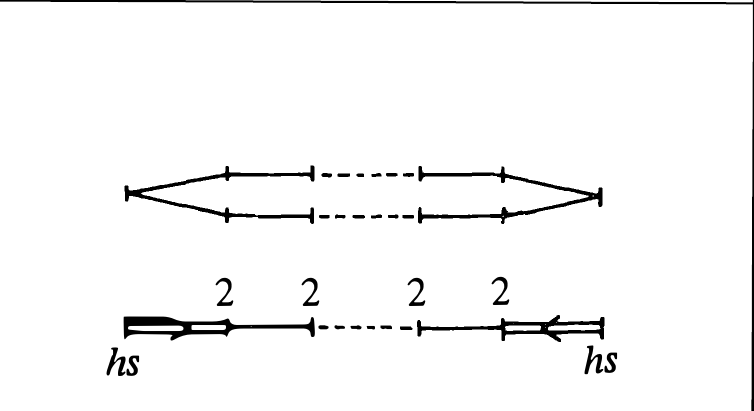
\includegraphics[width=\linewidth]{figures/02-class-66-1-066.png} & ${}^2A_{2m-1,m}^{(1)}$\\[8pt]
${}^2A^{\prime\prime}_{2m-1}\ (m\geq3)$ & $C\text{-}BC_{m-1}^{\mathrm{II}}$ & 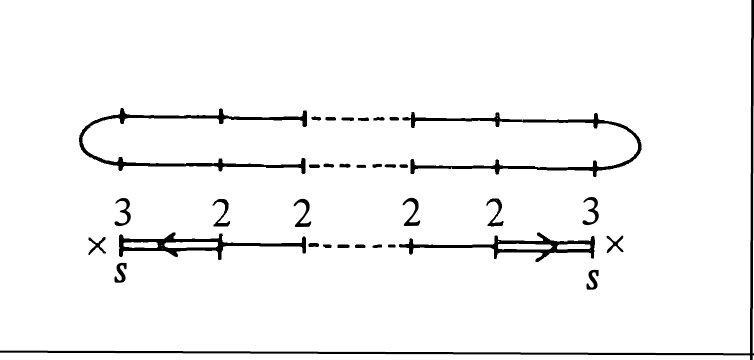
\includegraphics[width=\linewidth]{figures/02-class-66-2-066.png} & ${}^2A_{2m-1,m-1}^{(1)}$\\[8pt]
${}^2A^{\prime\prime}_3$ & $C\text{-}BC_1^{\mathrm{II}}$ & 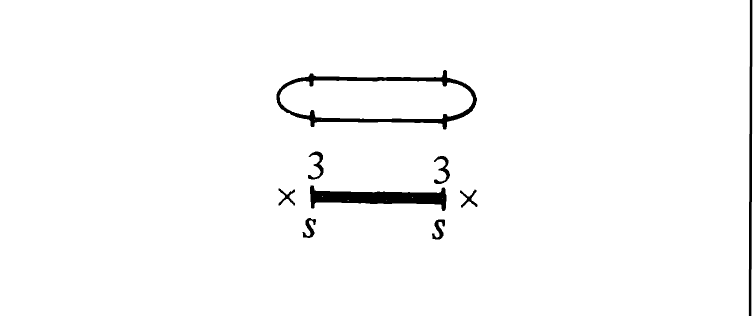
\includegraphics[width=\linewidth]{figures/02-class-66-3-066.png} & ${}^2A_{3,1}^{(1)}$\\[8pt]
${}^2A^{\prime}_{2m}\ (m\geq2)$ & $C\text{-}BC_m^{\mathrm{IV}}$ & 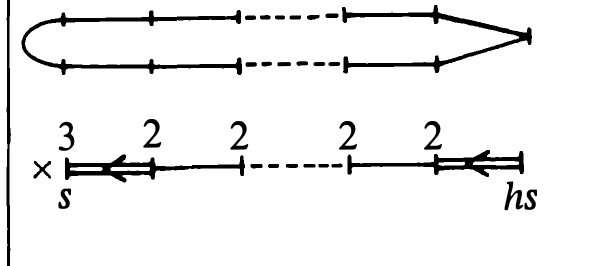
\includegraphics[width=\linewidth]{figures/02-class-67-1-067.png} & ${}^2A_{2m,m}^{(1)}$\\[8pt]
${}^2A^{\prime}_2$ & $C\text{-}BC_1^{\mathrm{IV}}$ & 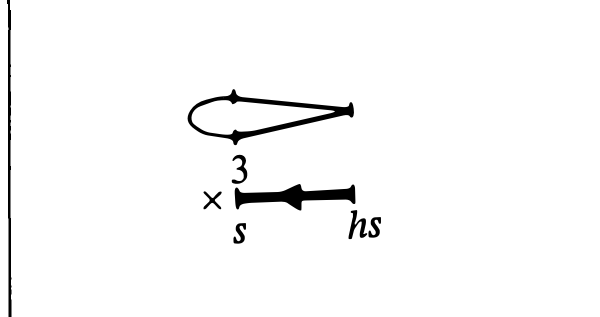
\includegraphics[width=\linewidth]{figures/02-class-67-2-067.png} & ${}^2A_{2,1}^{(1)}$\\[8pt]
${}^2B_n\ (n\geq3)$ & $C\text{-}B_{n-1}$ & 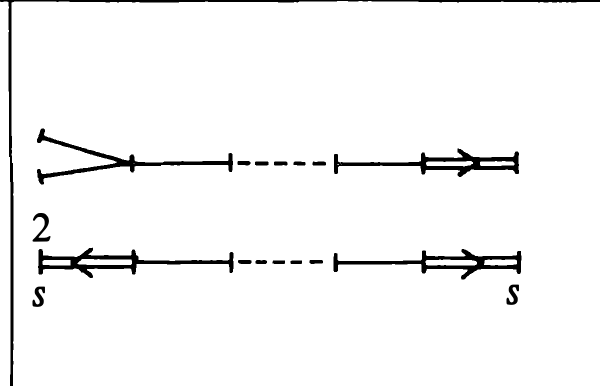
\includegraphics[width=\linewidth]{figures/02-class-67-3-067.png} & $B_{n,n-1}$\\[8pt]
${}^2B\text{-}C_n\ (n\geq3)$ & $C\text{-}BC_{n-1}^{\mathrm{III}}$ & 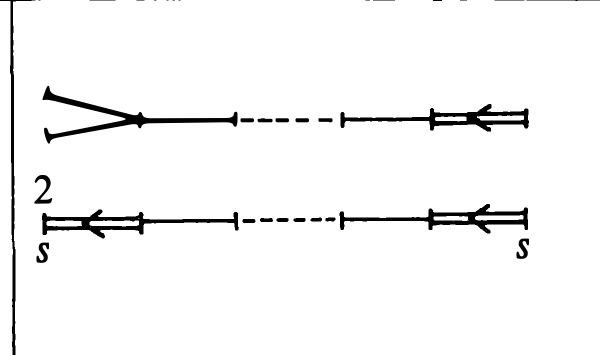
\includegraphics[width=\linewidth]{figures/02-class-67-4-067.png} & ${}^2A_{2n-1,n-1}^{(1)}$\\[8pt]
${}^2C_{2m-1}\ (m\geq3)$ & $C\text{-}BC_{m-1}^{\mathrm{IV}}$ & 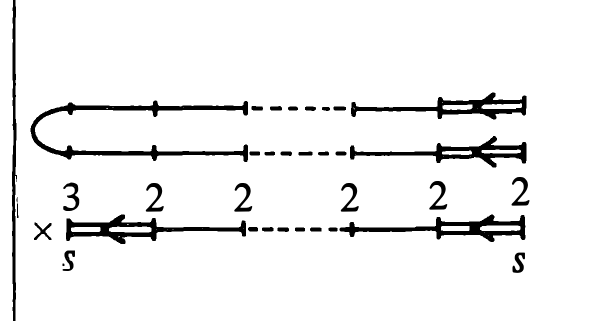
\includegraphics[width=\linewidth]{figures/02-class-67-5-067.png} & $C_{2m-1,m-1}^{(2)}$\\[8pt]
${}^2C_3$ & $C\text{-}BC_1^{\mathrm{IV}}$ & 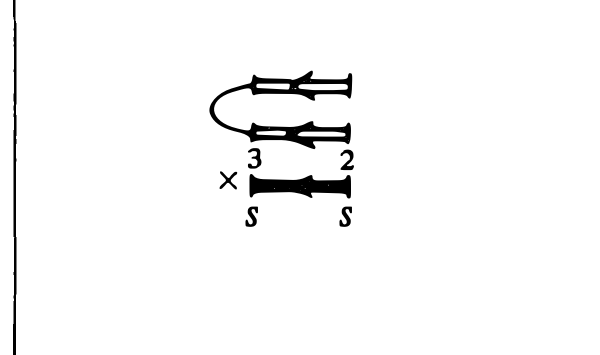
\includegraphics[width=\linewidth]{figures/02-class-67-6-067.png} & $C_{3,1}^{(2)}$\\[8pt]
${}^2C_{2m}\ (m\geq2)$ & $C_m$ & 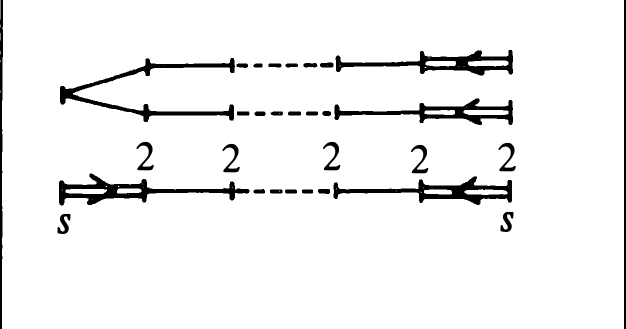
\includegraphics[width=\linewidth]{figures/02-class-68-1-068.png} & $C_{2m,m}^{(2)}$\\[8pt]
${}^2C_2$ & $A_1$ & 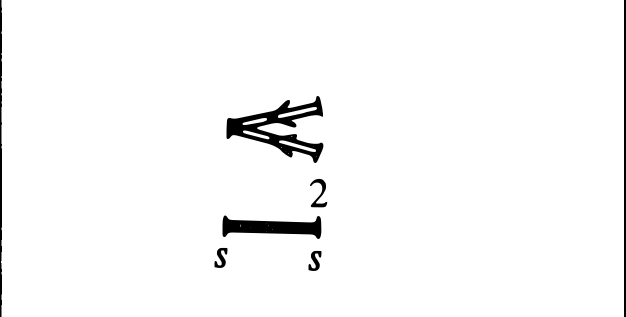
\includegraphics[width=\linewidth]{figures/02-class-68-2-068.png} & $C_{2,1}^{(2)}$\\[8pt]
${}^2C\text{-}B_{2m-1}\ (m\geq3)$ & $C\text{-}BC_{m-1}^{\mathrm I}$ & 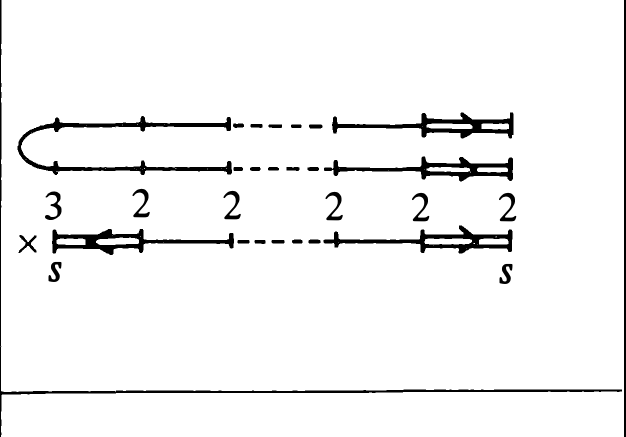
\includegraphics[width=\linewidth]{figures/02-class-68-3-068.png} & ${}^2D_{2m,m-1}^{(2)}$\\[8pt]
${}^2C\text{-}B_3$ & $C\text{-}BC_1^{\mathrm I}$ & 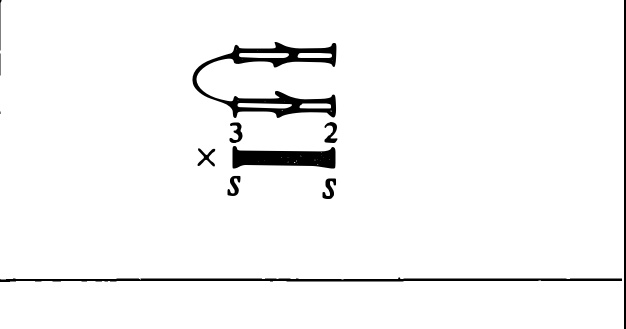
\includegraphics[width=\linewidth]{figures/02-class-68-4-068.png} & ${}^2D_{4,1}^{(2)}$\\[8pt]
${}^2C\text{-}B_{2m}\ (m\geq2)$ & $C\text{-}BC_m^{\mathrm{III}}$ & 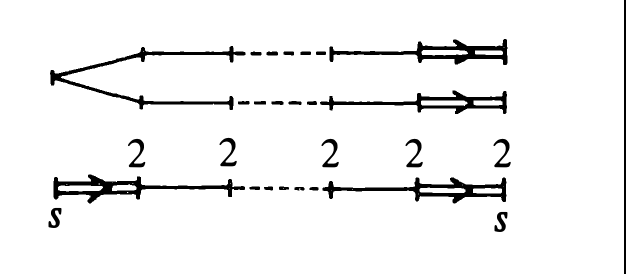
\includegraphics[width=\linewidth]{figures/02-class-68-5-068.png} & ${}^2D_{2m+1,m}^{(2)}$\\[8pt]
${}^2C\text{-}B_2$ & $C\text{-}BC_1^{\mathrm{III}}$ & 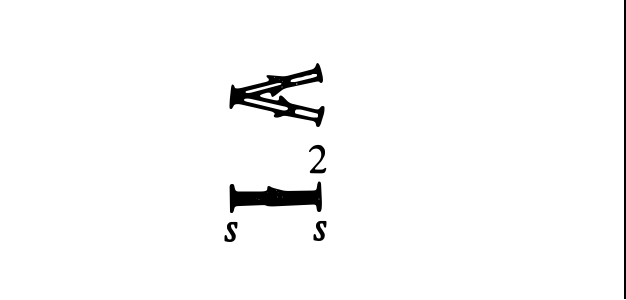
\includegraphics[width=\linewidth]{figures/02-class-68-6-068.png} & ${}^2D_{3,1}^{(2)}$\\[8pt]
${}^2D_n\ (n\geq4)$ & $B_{n-1}$ & 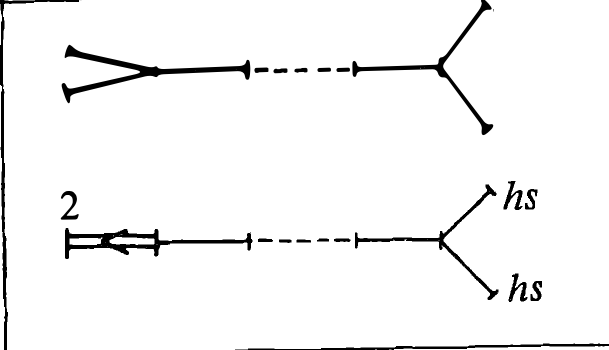
\includegraphics[width=\linewidth]{figures/02-class-69-1-069.png} & ${}^2D_{n,n-1}^{(1)}$\\[8pt]
${}^2D^{\prime}_n\ (n\geq4)$ & $C\text{-}B_{n-2}$ & 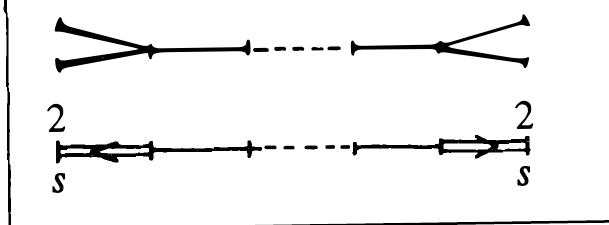
\includegraphics[width=\linewidth]{figures/02-class-69-2-069.png} & ${}^1D_{n,n-2}^{(1)}$\\[8pt]
${}^2D^{\prime\prime}_{2m}\ (m\geq3)$ & $B\text{-}C_m$ & 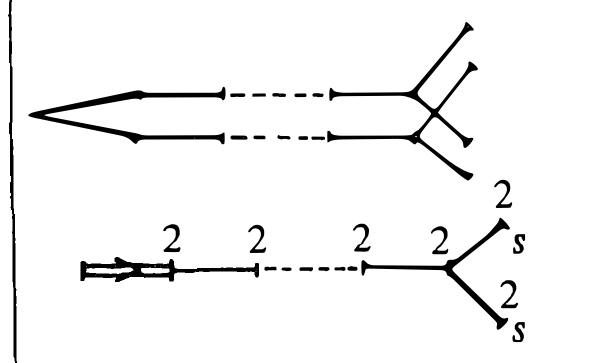
\includegraphics[width=\linewidth]{figures/02-class-69-3-069.png} & ${}^1D_{2m,m}^{(2)}$\\[8pt]
${}^2D^{\prime\prime}_{2m+1}\ (m\geq3)$ & $B\text{-}BC_m$ & 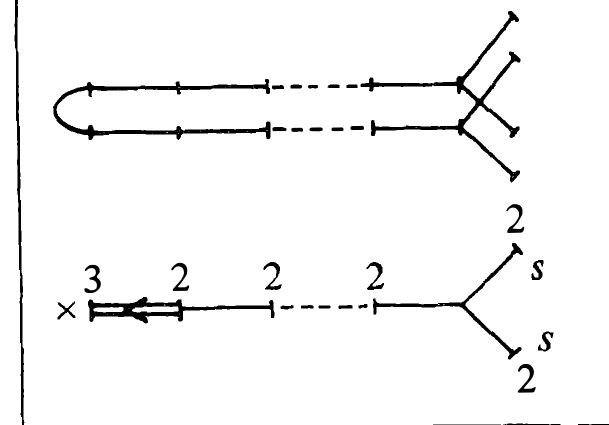
\includegraphics[width=\linewidth]{figures/02-class-69-4-069.png} & ${}^2D_{2m+1,m}^{(2)}$\\[8pt]
${}^2D^{\prime\prime}_5$ & $B\text{-}BC_2$ & 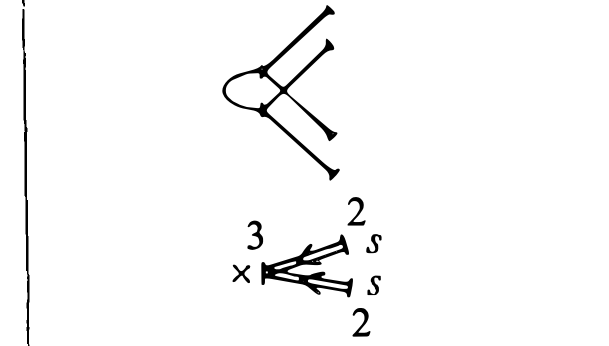
\includegraphics[width=\linewidth]{figures/02-class-69-5-069.png} & ${}^2D_{5,2}^{(2)}$\\[8pt]
${}^3D_4$ & $G_2$ & 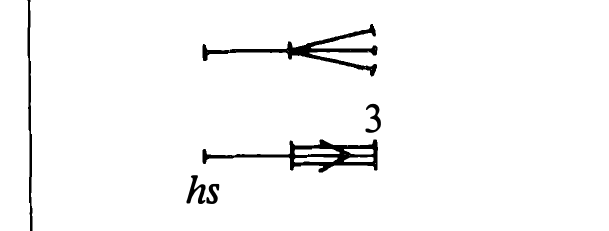
\includegraphics[width=\linewidth]{figures/02-class-69-6-069.png} & ${}^3D_{4,2}$\\[8pt]
${}^4D_{2m}\ (m\geq3)$ & $C\text{-}BC_{m-1}^{\mathrm{III}}$ & 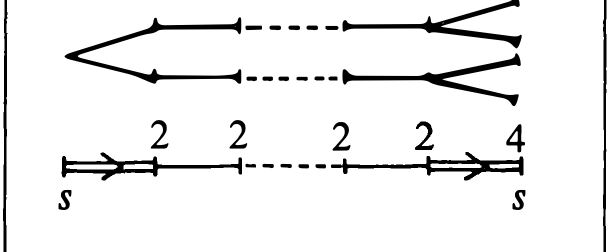
\includegraphics[width=\linewidth]{figures/02-class-70-1-070.png} & ${}^2D_{2m,m-1}^{(2)}$\\[8pt]
${}^4D_4$ & $C\text{-}BC_1^{\mathrm{III}}$ & 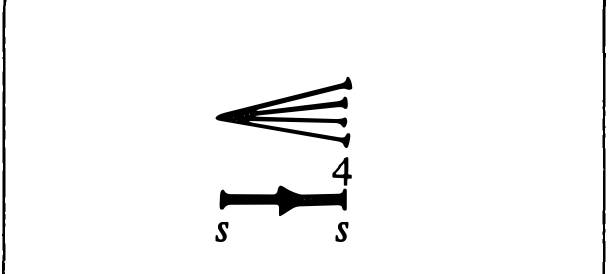
\includegraphics[width=\linewidth]{figures/02-class-70-2-070.png} & ${}^2D_{4,1}^{(2)}$\\[8pt]
${}^4D_{2m+1}\ (m\geq3)$ & $C\text{-}BC_{m-1}^{\mathrm I}$ & 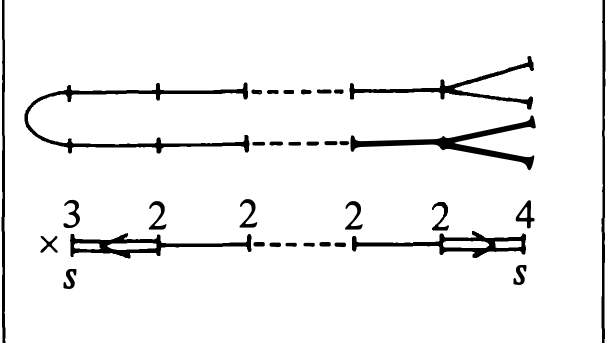
\includegraphics[width=\linewidth]{figures/02-class-70-3-070.png} & ${}^1D_{2m+1,m-1}^{(2)}$\\[8pt]
${}^4D_5$ & $C\text{-}BC_1^{\mathrm I}$ & 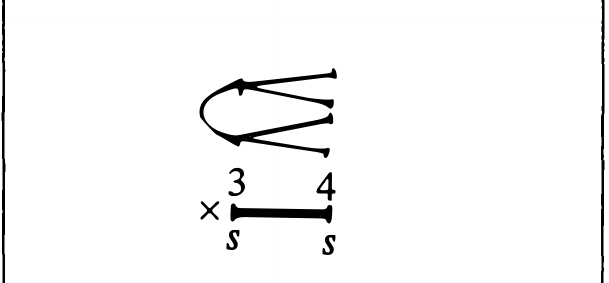
\includegraphics[width=\linewidth]{figures/02-class-70-4-070.png} & ${}^1D_{5,1}^{(2)}$\\[8pt]
${}^2E_6$ & $F_4$ & 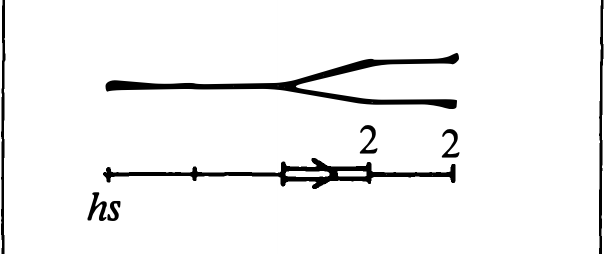
\includegraphics[width=\linewidth]{figures/02-class-70-5-070.png} & ${}^2E_{6,4}^2$\\[8pt]
${}^3E_6$ & $G_2^{\mathrm I}$ & 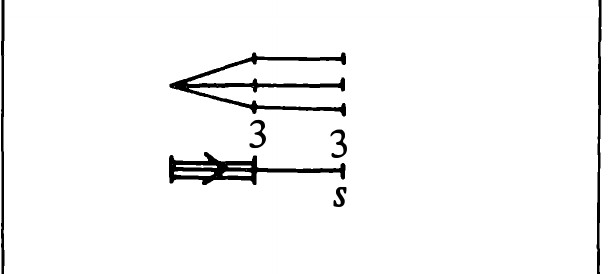
\includegraphics[width=\linewidth]{figures/02-class-70-6-070.png} & ${}^1E_{6,2}^{16}$\\[8pt]
${}^2E_7$ & $F_4^{\mathrm I}$ & 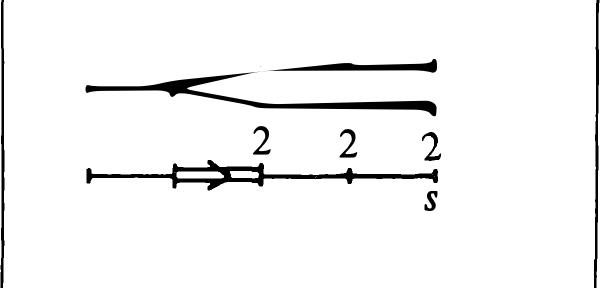
\includegraphics[width=\linewidth]{figures/02-class-70-7-070.png} & $E_{7,4}^9$\\[8pt]
\bottomrule
\end{longtable}
\noindent ${}^2D''_5$ 一行的仿射根系 $B$-$BC_2$：原注指出，这一 échelonnage 在 [8，第 29 页] 的表中遗漏。
\origsubsection{4.4}{解释（Interpretation）}
下面用经典术语重新表述这一分类，为 $K$ 上绝对拟单群的每个中心同源类选取一个代表，并在每种情形给出相应类型名称，记号同表 4.2、4.3 第一列。

$K$ 上 $d^2$ 维中心除代数的特殊线性群（special linear group）$\SL_m$，$md\geq2$。类型为 ${}^dA_{md-1}$。

$K$ 的二次扩张 $L$ 上 $r$ 个变量的 Hermite 型 $h$（$r\geq3$）、Witt 指标（Witt index）为 $r'$ 的特殊酉群（special unitary group）$\operatorname{SU}(h)$。如果 $L/K$ 分歧，假设 $r\ne4$；因为 $r=4$ 的情形，在 $r'=2$ 或 $1$ 时，分别更适合用六个变量的通常特殊正交群，或三个变量的四元数特殊正交群表示。若型 $h$ 分裂，则当 $L/K$ 非分歧时类型为 ${}^2A'_{r-1}$；否则为 $C$-$BC_n$（$r=2n+1$）或 $B$-$C_n$（$r=2n$）。若 $h$ 不分裂，则 $r=2r'+2$，当 $L/K$ 非分歧或分歧时，类型分别为 ${}^2A''_{r-1}$ 或 ${}^2B$-$C_{r'+1}$。

$K$ 上 $r$ 个变量的二次型 $q$（$r\geq6$）、Witt 指标为 $r'$ 的特殊正交群（special orthogonal group）$\operatorname{SO}(q)$。若 $r$ 为偶数，以 $L$ 表示 $q$ 的偶 Clifford 代数（even Clifford algebra）的中心，它同构于 $K\oplus K$（型 $q$ 的判别式为一或 Arf 不变量为零），或为 $K$ 的二次扩张。若 $L/K$ 非分歧（特别是 $L=K\oplus K$），假设 $r\ne6$，因为 $r=6$ 更适合由四个变量的特殊酉群表示。若 $r=2r'$（$2r'+1$），类型为 $D_{r'}$（$B_{r'}$）。若 $r=2r'+2$，则 $L$ 为 $K$ 的二次扩张，当 $L/K$ 非分歧或分歧时，类型分别为 ${}^2D_{r'+1}$ 或 $C$-$B_{r'}$。最后，若 $r=2r'+3$（$2r'+4$），类型为 ${}^2B_{r'+1}$（${}^2D'_{r'+2}$）。

$2n\geq4$ 个变量的辛群（symplectic group）类型为 $C_n$。

关于标准对合（standard involution）的 $r$ 个变量的四元数 Hermite 型（quaternion hermitian form）的特殊酉群，$r\geq2$。Witt 指标总是最大的，类型为 ${}^2C_r$。

关于四元数代数对合 $\sigma$ 的 $r$ 个变量的四元数 $\sigma$ 二次型（quaternionic $\sigma$-quadratic form）的特殊正交群 $\operatorname{SO}(q)$，$r\geq3$，其中该对合的对称元素空间为三维（见 [21]、[23]；若 $\operatorname{char}K\ne2$，“$\sigma$ 二次”即“$\sigma$ Hermite”，该群也是一个关于标准对合的反 Hermite 型的特殊酉群）。令 $r'$ 为型的 Witt 指标，$L$ 为其“偶”Clifford 代数 $\operatorname{Cl}(q)$ 的中心（见 [21]）。若 $L/K$ 非分歧（特别是 $L\simeq K\oplus K$），假设 $r\ne3$，因为 $r=3$ 更适合由四个变量的特殊酉群表示；若进一步 $r=2r'$，还假设 $r\ne4$，因为 $r=2r'=4$ 通过三重性原理（triality principle），更适合由八个变量、Witt 指标为 $2$ 的通常特殊正交群表示。总有 $2r'\leq r\leq2r'+3$。若 $r=2r'$，则 $L\simeq K\oplus K$，群类型为 ${}^2D''_r$。若 $r=2r'+1$（$2r'+2$），则 $L$ 为 $K$ 的二次扩张；当 $L/K$ 非分歧或分歧时，类型分别为 ${}^2D''_r$（${}^4D_r$）或 ${}^2C$-$B_{r-1}$。若 $r=2r'+3$，则 $L\simeq K\oplus K$，类型为 ${}^4D_r$。

拟分裂三重性 $D_4$（quasi-split triality $D_4$）。令 $L$ 为分裂域，它是三次循环扩张，或 Galois 群为 $\mathfrak S_3$ 的六次 Galois 扩张。若 $L/K$ 非分歧（因而为三次循环扩张），类型为 ${}^3D_4$；否则为 $G_2^{\mathrm I}$。

分裂例外群（split exceptional groups）。类型名称与其绝对类型相同，即 $G_2$、$F_4$、$E_6$、$E_7$、$E_8$。

$E_6$ 型拟分裂群。其类型在二次分裂域 $L$ 非分歧或分歧时，分别为 ${}^2E_6$ 或 $F_4^{\mathrm I}$。

$E_6$、$E_7$ 型非拟分裂群。它们分别是借助维数为 $9$、$4$ 的中心除代数构造的 $E_6$、$E_7$ 的形式；类型为 ${}^3E_6$、${}^2E_7$。
\origsubsection{4.5}{不变量（Invariants）}
表 4.2、4.3 所列的全部群类型，在任何满足本文假设且剩余域有限的 $K$ 上都存在。给定名称对应的中心同源类总是唯一，只有下述例外。

$d\geq5$ 时，${}^dA_{md-1}$ 型的同源类，由 $K$ 上维数为 $d^2$ 的互为反代数的中心除代数对分类；因而其数目为 $\frac12\varphi(d)$，其中 $\varphi$ 为 Euler 函数。

$B$-$C_n$、${}^2B$-$C_n$、$C$-$B_n$、${}^2C$-$B_n$、$C$-$BC_n$ 及 $F_4^{\mathrm I}$ 型的同源类，由 $K$ 的分歧二次扩张分类，即 4.4 中一直记为 $L$ 的扩张。

$G_2^{\mathrm I}$ 型的群，由 $K$ 的 Galois 扩张 $L$ 分类，其中 $L/K$ 为三次循环扩张，或六次非循环扩张。\footnote{\textbf{译者注（本次校订）：}这里还须要求 $L/K$ 分歧。按照4.4的区分，非分歧三次循环扩张对应的是 ${}^3D_4$，而非 $G_2^{\mathrm I}$。}
\origsubsection{4.6}{分类工具包（The classification kit）}
下面的规律提供了一种重建分类的便捷方法。首先，除 ${}^dA_{d-1}$ 外，表 4.2、4.3 的每种类型均由局部 Dynkin 图及其所带整数 $d(v)$ 完全刻画。现在考虑一个秩（顶点数）至少为三的仿射型连通 Coxeter 图，为每个顶点附上一个整数，在某些顶点标叉（也可以一个都不标），并用箭头将每条双线或三线定向。则存在半单群 $G$，其相对局部 Dynkin 图为所得图、且给定整数为 $d(v)$，当且仅当由每对顶点构成的所有子图均属于下列类型之一。这些图代表相对秩为二的拟分裂群的通常 Dynkin 图：
\begin{center}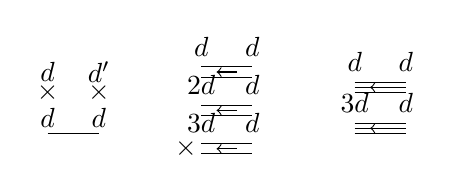
\begin{tikzpicture}[x=.65cm,y=.65cm]
\node at(0,1.1){$d$};\node at(1,1.1){$d'$};\node at(0,.7){$\times$};\node at(1,.7){$\times$};
\draw(0,-.1)--(1,-.1);\node at(0,.2){$d$};\node at(1,.2){$d$};
\foreach\y/\a in {1.1/d,.35/2d,-.4/3d}{
\draw(3,\y-.1)--(4,\y-.1) (3,\y+.1)--(4,\y+.1);\draw[->](3.7,\y)--(3.3,\y);
\node[above]at(3,\y+.12){$\a$};\node[above]at(4,\y+.12){$d$};}
\node at(2.7,-.4){$\times$};
\foreach\y/\a in {.8/d,0/3d}{
\draw(6,\y-.1)--(7,\y-.1) (6,\y)--(7,\y) (6,\y+.1)--(7,\y+.1);\draw[->](6.7,\y)--(6.3,\y);
\node[above]at(6,\y+.12){$\a$};\node[above]at(7,\y+.12){$d$};}
\end{tikzpicture}
\end{center}
而且，群 $G$ 可选为绝对拟单，当且仅当各整数 $d(v)$ 互素，或底层 Coxeter 图为环。至于相对秩为一、底层 Coxeter 图为粗边的类型，它们可作为更高秩类型的“极限情形”得到，这里不再详述。
\begin{thebibliography}{99}
\bibitem[1]{c02-1} A. Borel, \emph{Admissible representations of a semi-simple group over a local field with vectors fixed under an Iwahori subgroup}, Invent. Math. 35 (1976), 233--259.
\bibitem[2]{c02-2} A. Borel et J.-P. Serre, \emph{Cohomologie d'immeubles et de groupes S-arithmétiques}, Topology 15 (1976), 211--232.
\bibitem[3]{c02-3} A. Borel et J. Tits, \emph{Groupes réductifs}, Publ. Math. Inst. Hautes Études Scientifiques 27 (1965), 55--150.
\bibitem[4]{c02-4} A. Borel et J. Tits, \emph{Compléments à l'article ``Groupes réductifs''}, Publ. Math. Inst. Hautes Études Scientifiques 41 (1972), 253--276.
\bibitem[5]{c02-5} N. Bourbaki, \emph{Groupes et algèbres de Lie}, Chap. IV, V, VI, Hermann, Paris, 1968.
\bibitem[6]{c02-6} F. Bruhat et J. Tits, (a) \emph{BN-paires de type affine et données radicielles}, C. R. Acad. Sci. Paris 263 (1966), 598--601; (b) \emph{Groupes simples résiduellement déployés sur un corps local}, 同刊，766--768; (c) \emph{Groupes algébriques simples sur un corps local}, 同刊，822--825; (d) \emph{Groupes algébriques simples sur un corps local: cohomologie galoisienne, décompositions d'Iwasawa et de Cartan}, 同刊，867--869.
\bibitem[7]{c02-7} F. Bruhat et J. Tits, \emph{Groupes algébriques simples sur un corps local}, Proc. Conf. on Local Fields (Driebergen, 1966), Springer, New York, 1967, pp. 23--36.
\bibitem[8]{c02-8} F. Bruhat et J. Tits, \emph{Groupes réductifs sur un corps local. I, Données radicielles valuées}, Publ. Math. Inst. Hautes Études Scientifiques 41 (1972), 5--251.
\bibitem[9]{c02-9} F. Bruhat et J. Tits, \emph{Groupes réductifs sur un corps local. II, Schémas en groupes}（准备中）。
\bibitem[10]{c02-10} C. Chevalley, \emph{Sur certains groupes simples}, Tôhoku Math. J. 7 (1955), 14--66.
\bibitem[11]{c02-11} M. Demazure et A. Grothendieck, \emph{Schémas en groupes. III}, Sém. Géom. Alg. 1962/64, Lecture Notes in Math., vol. 153, Springer, New York, 1970.
\bibitem[12]{c02-12} O. Goldman et N. Iwahori, \emph{The space of p-adic norms}, Acta Math. 109 (1963), 137--177.
\bibitem[13]{c02-13} H. Hijikata, \emph{On the arithmetic of p-adic Steinberg groups}, 油印讲义，Yale Univ., 1964.
\bibitem[14]{c02-14} H. Hijikata, \emph{On the structure of semi-simple algebraic groups over valuation fields. I}, Japan. J. Math. 1 (1975), 225--300.
\bibitem[15]{c02-15} N. Iwahori and H. Matsumoto, \emph{On some Bruhat decomposition and the structure of the Hecke ring of p-adic Chevalley groups}, Publ. Math. Inst. Hautes Études Scientifiques 25 (1965), 5--48.
\bibitem[16]{c02-16} M. Kneser, \emph{Galois-Kohomologie halbeinfacher algebraischer Gruppen über p-adischen Körpern}, Math. Z. 88 (1965), 40--47; 89 (1965), 250--272.
\bibitem[17]{c02-17} I. G. MacDonald, \emph{Affine root systems and Dedekind's $\eta$ function}, Invent. Math. 15 (1972), 91--143.
\bibitem[18]{c02-18} G. Prasad, \emph{Lattices in semi-simple groups over local fields}, Advances in Math.（即将发表）。
\bibitem[19]{c02-19} G. Rousseau, \emph{Immeubles des groupes réductifs sur les corps locaux}, 博士论文，Paris XI (1977).
\bibitem[20]{c02-20} T. A. Springer, \emph{Reductive groups}, 本论文集，第 1 册，第 3--27 页。
\bibitem[21]{c02-21} J. Tits, \emph{Formes quadratiques, groupes orthogonaux et algèbres de Clifford}, Invent. Math. 5 (1968), 19--41.
\bibitem[22]{c02-22} J. Tits, \emph{Classification of algebraic semisimple groups}, Proc. Summer Inst. on Algebraic Groups and Discontinuous Groups (Boulder, 1965), Proc. Sympos. Pure Math., vol. 9, Amer. Math. Soc., Providence, R. I., 1966, pp. 33--62.
\bibitem[23]{c02-23} J. Tits, \emph{Buildings of spherical type and finite BN-pairs}, Lecture Notes in Math., vol. 386, Springer, New York, 1974.
\bibitem[24]{c02-24} J. Tits, \emph{On buildings and their applications}, Proc. Internat. Congr. Math. (Vancouver, 1974), vol. 1, Canad. Math. Congr., 1975, pp. 209--220.
\bibitem[25]{c02-25} J. Tits, \emph{Résumé de cours}, Annuaire du Collège de France pour 1975--1976, pp. 49--56.
\bibitem[26]{c02-26} J. Tits, \emph{Classification of buildings of spherical type and Moufang polygons: a survey}, Coll. Intern. Teorie Combinatorie (Rome, 1973), Atti dei Convegni Lincei 17 (1976), 229--246.
\end{thebibliography}
\par\noindent 巴黎，法兰西学院（Collège de France）。

